\documentclass{beamer}
\usetheme{Boadilla}
\usefonttheme{professionalfonts}
\usepackage{lmodern}
\usepackage{graphicx}
\usepackage[space]{grffile}

\title{Inputs for MyLake-Sediment Model}
\subtitle{Lake Erie}
\author{I. Markelov, B. McNeil}
\institute{Ecohydrology}
\date{\today}

\graphicspath{ {../../post_proc_scripts/plots/} }

\begin{document}

\begin{frame}
\titlepage
\end{frame}


\begin{frame}
\frametitle{Outline:}
\begin{center}
\tableofcontents
\end{center}
\end{frame}

\section{Weather}
\label{sec:weather}

\subsection{Western Basin}
\label{sub:wes}

\begin{frame}
\frametitle{Weather: Western Basin}

\begin{figure}
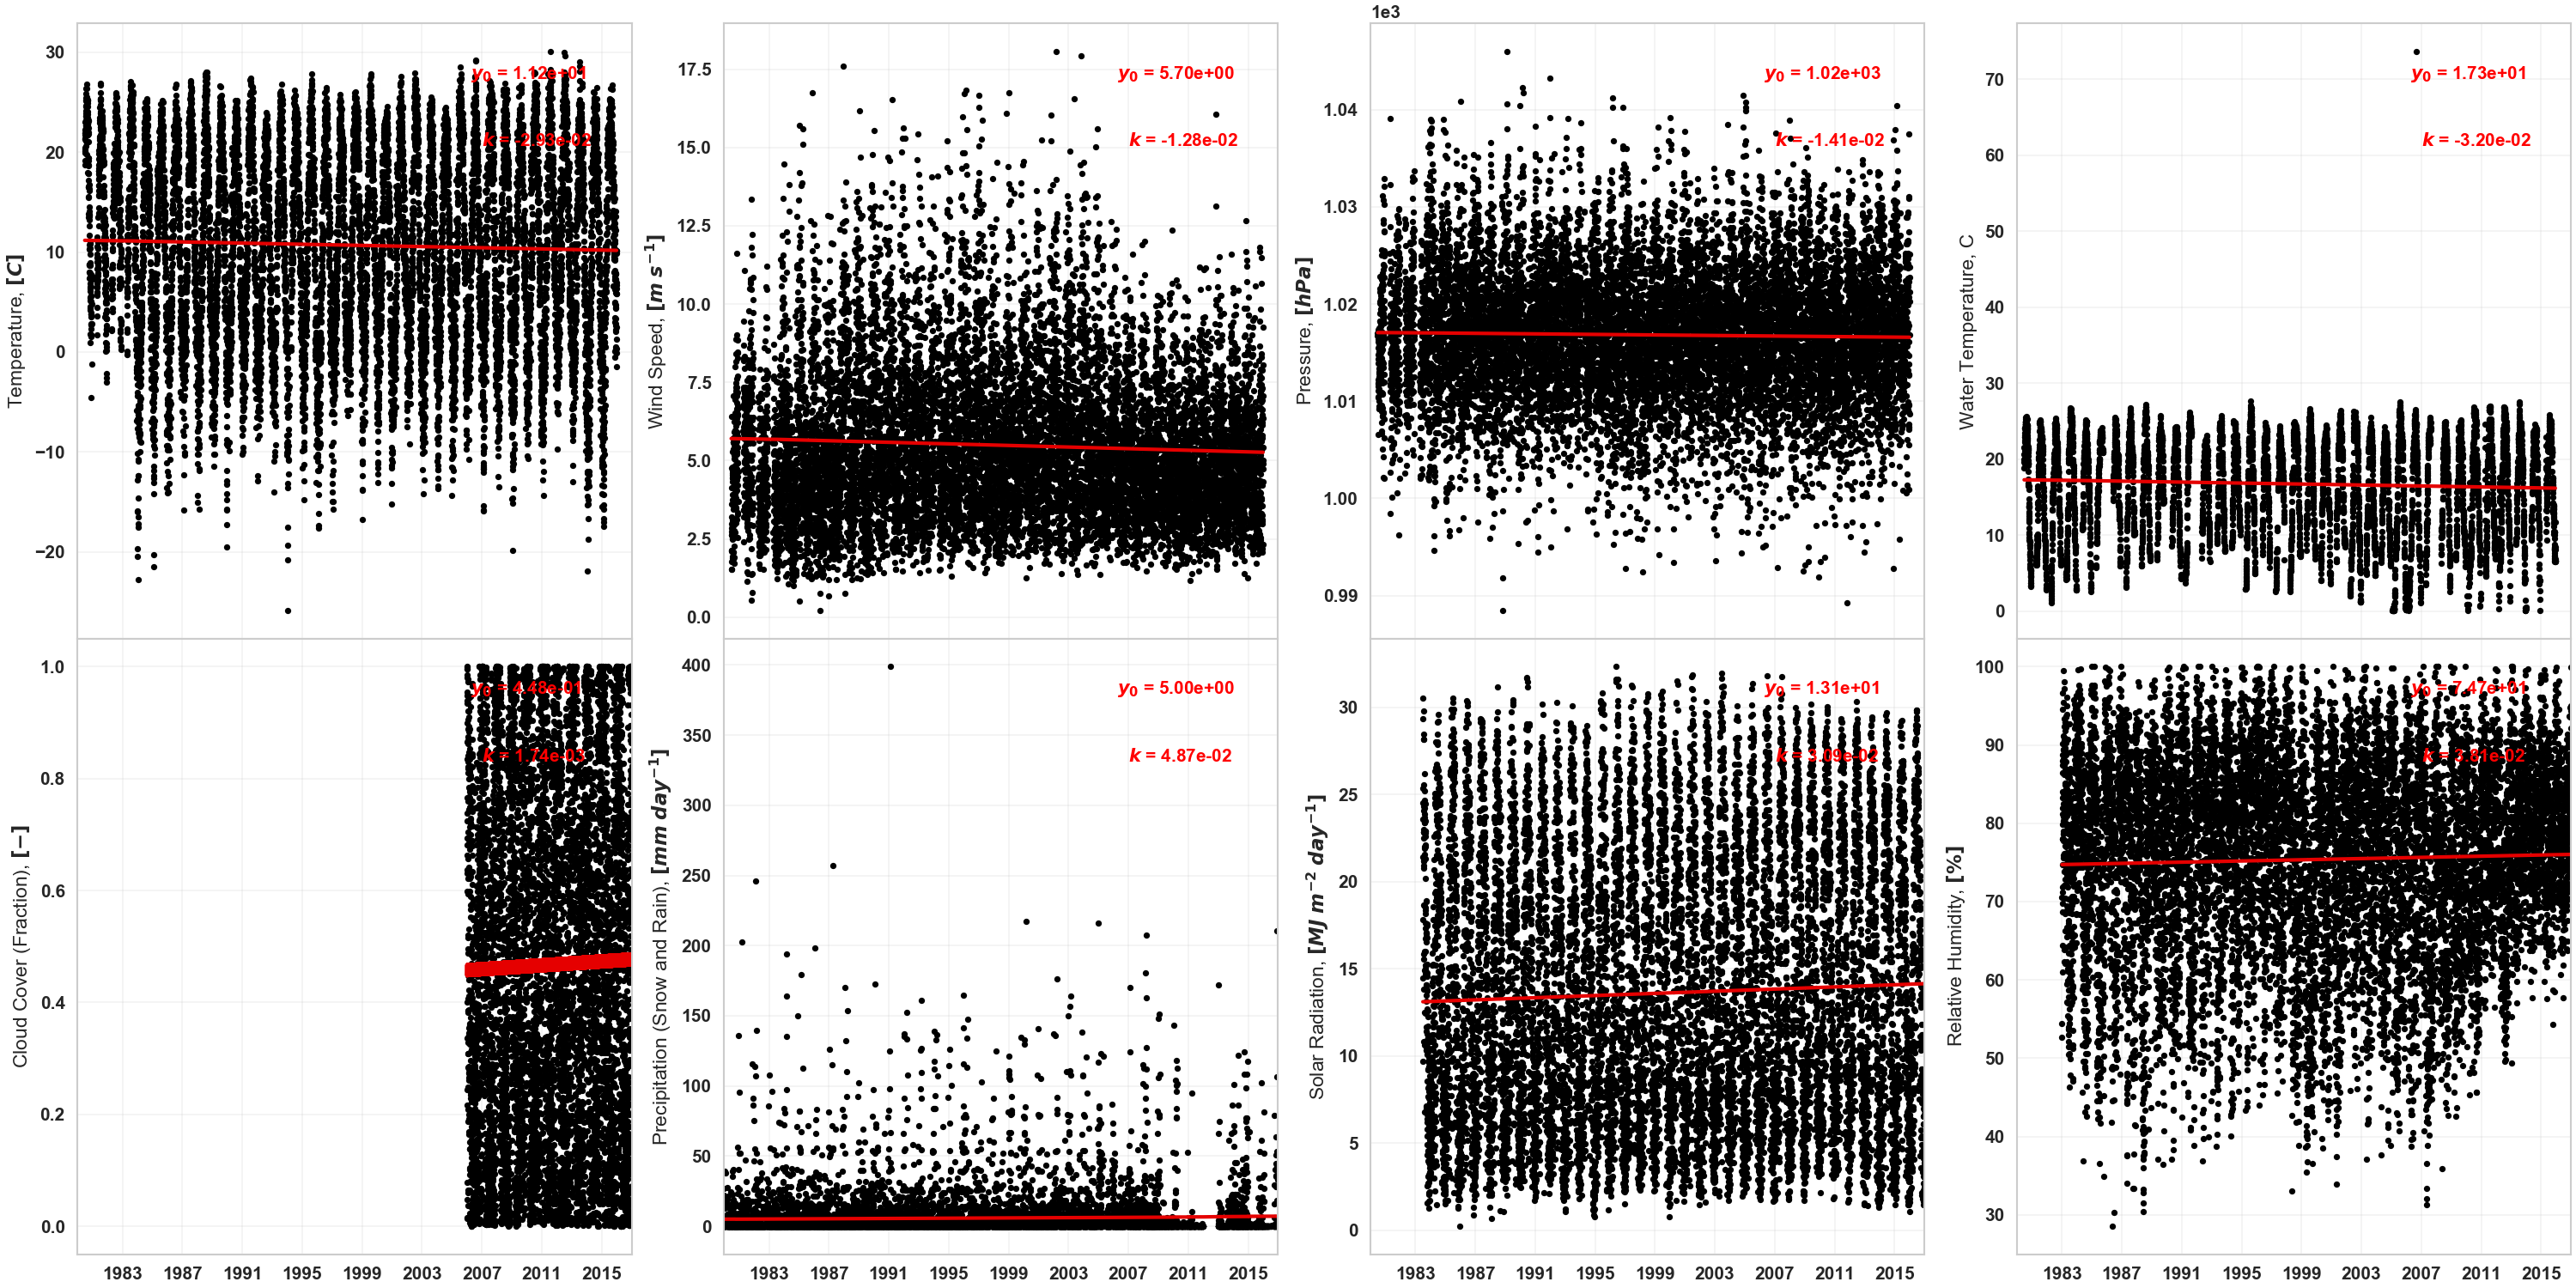
\includegraphics[width=\textwidth]{weather/western basin weather.png}
\end{figure}

\end{frame}

\subsection{Central Basin}
\label{sub:cen}

\begin{frame}
\frametitle{Weather: Central Basin}

\begin{figure}
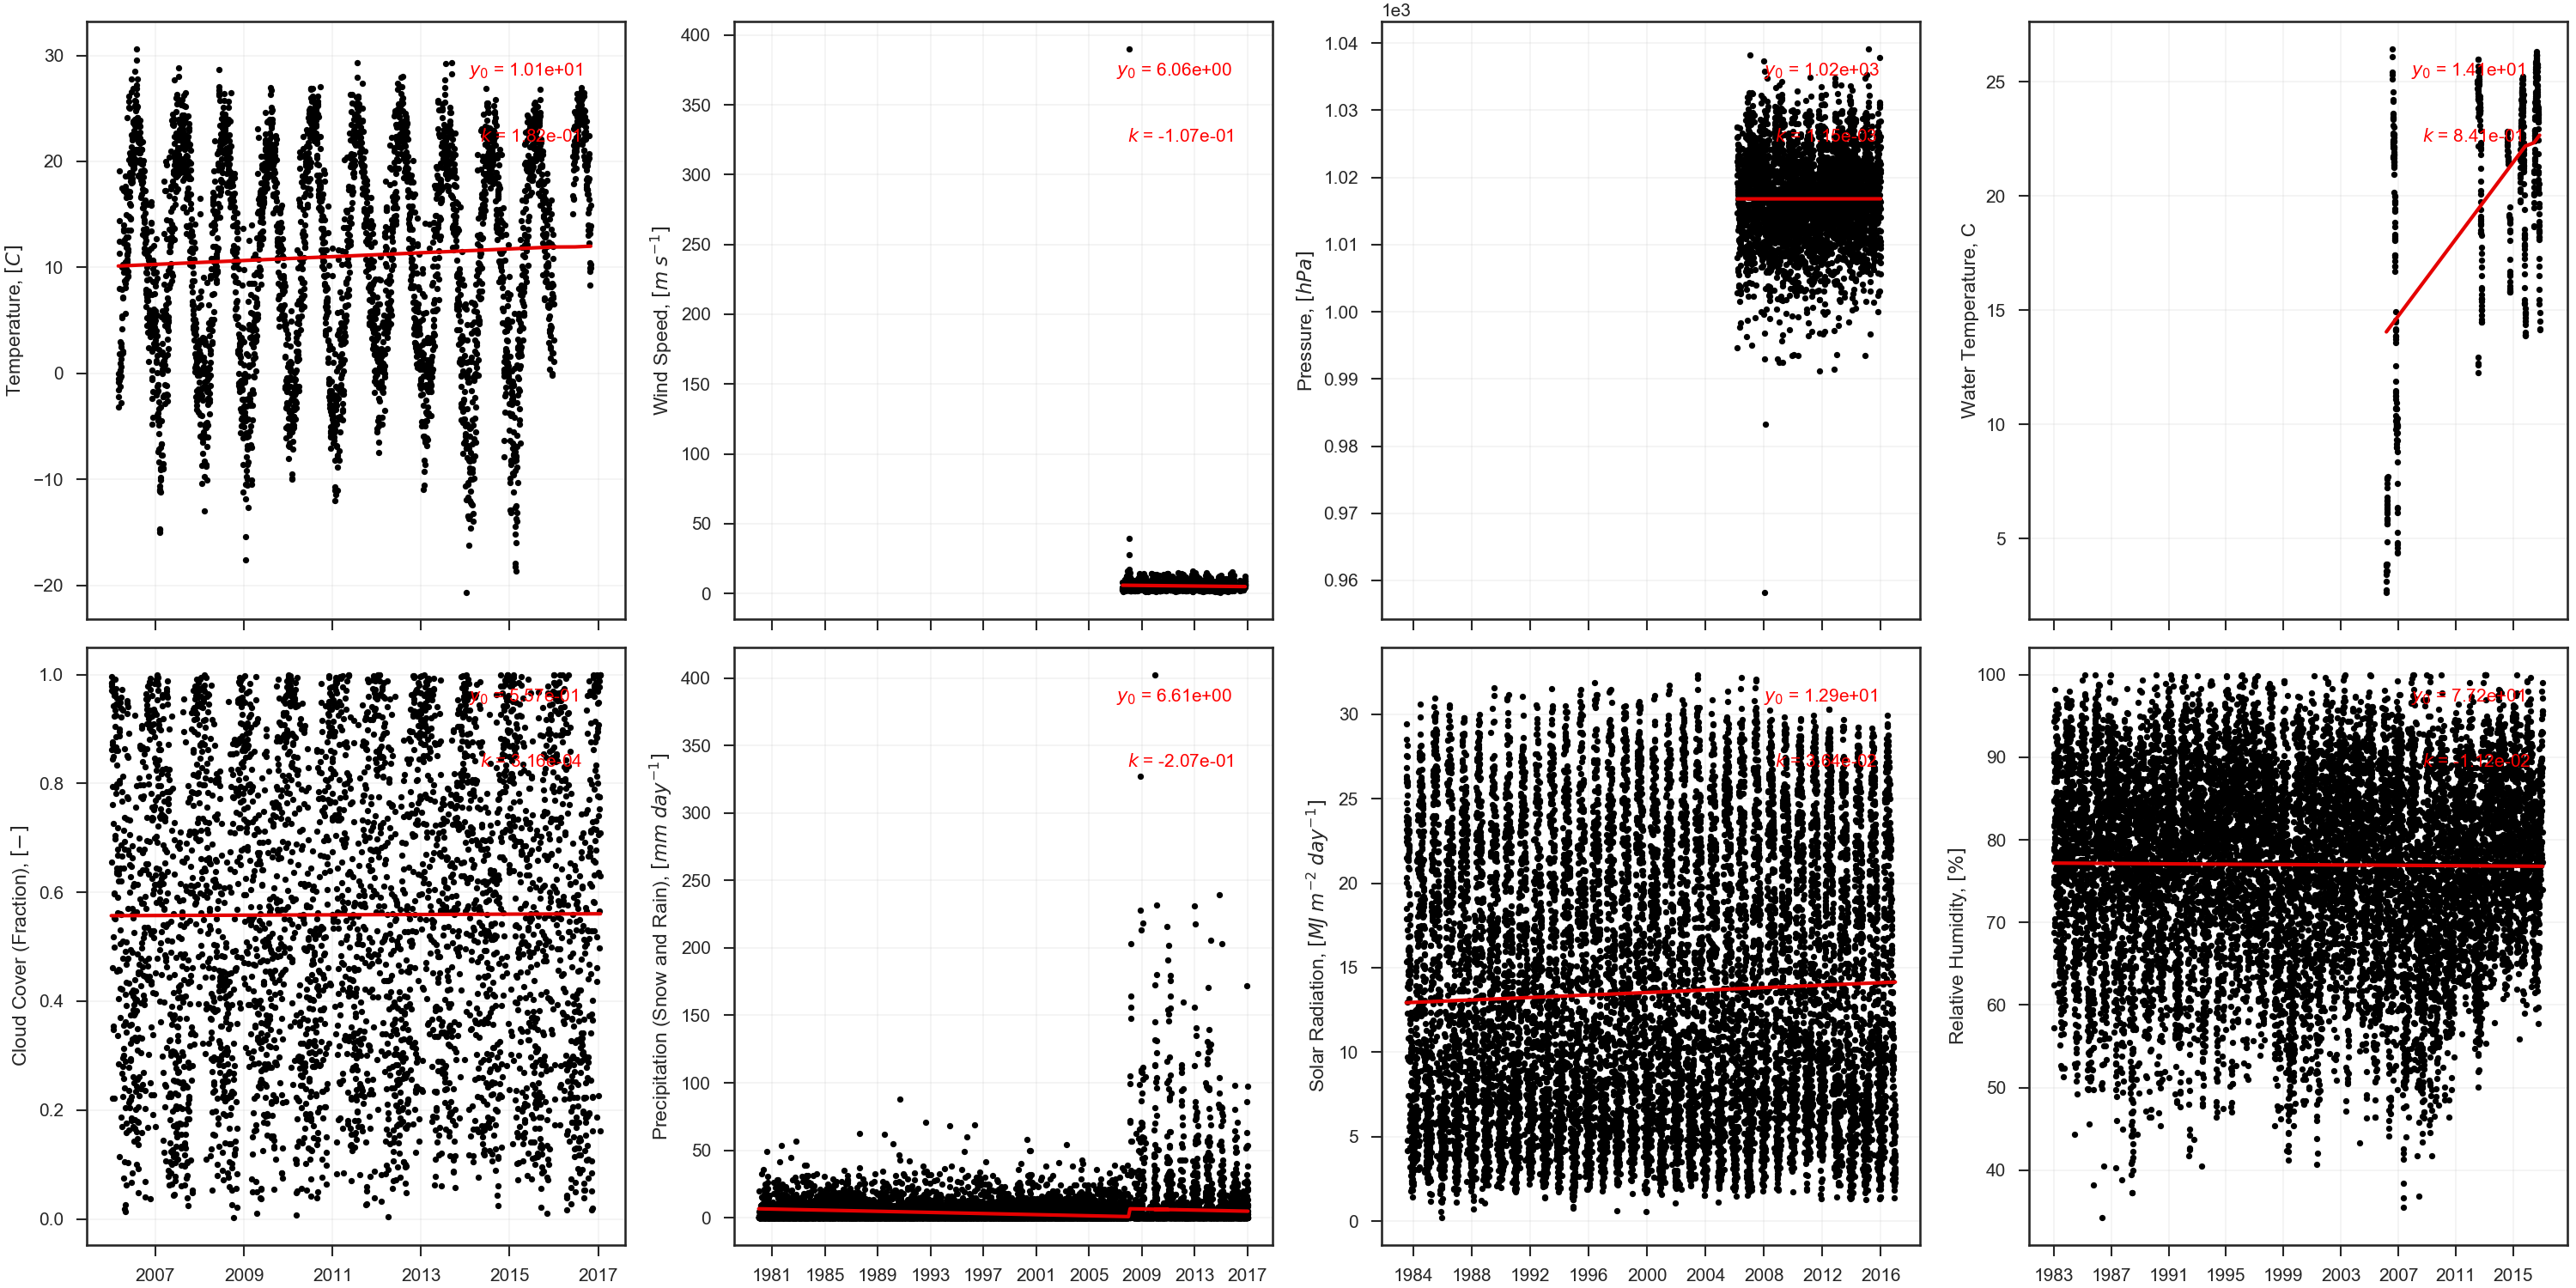
\includegraphics[width=\textwidth]{weather/central basin weather.png}
\end{figure}

\end{frame}

\subsection{Easter Basin}
\label{sub:wes}

\begin{frame}
\frametitle{Weather: Eastern Basin}

\begin{figure}
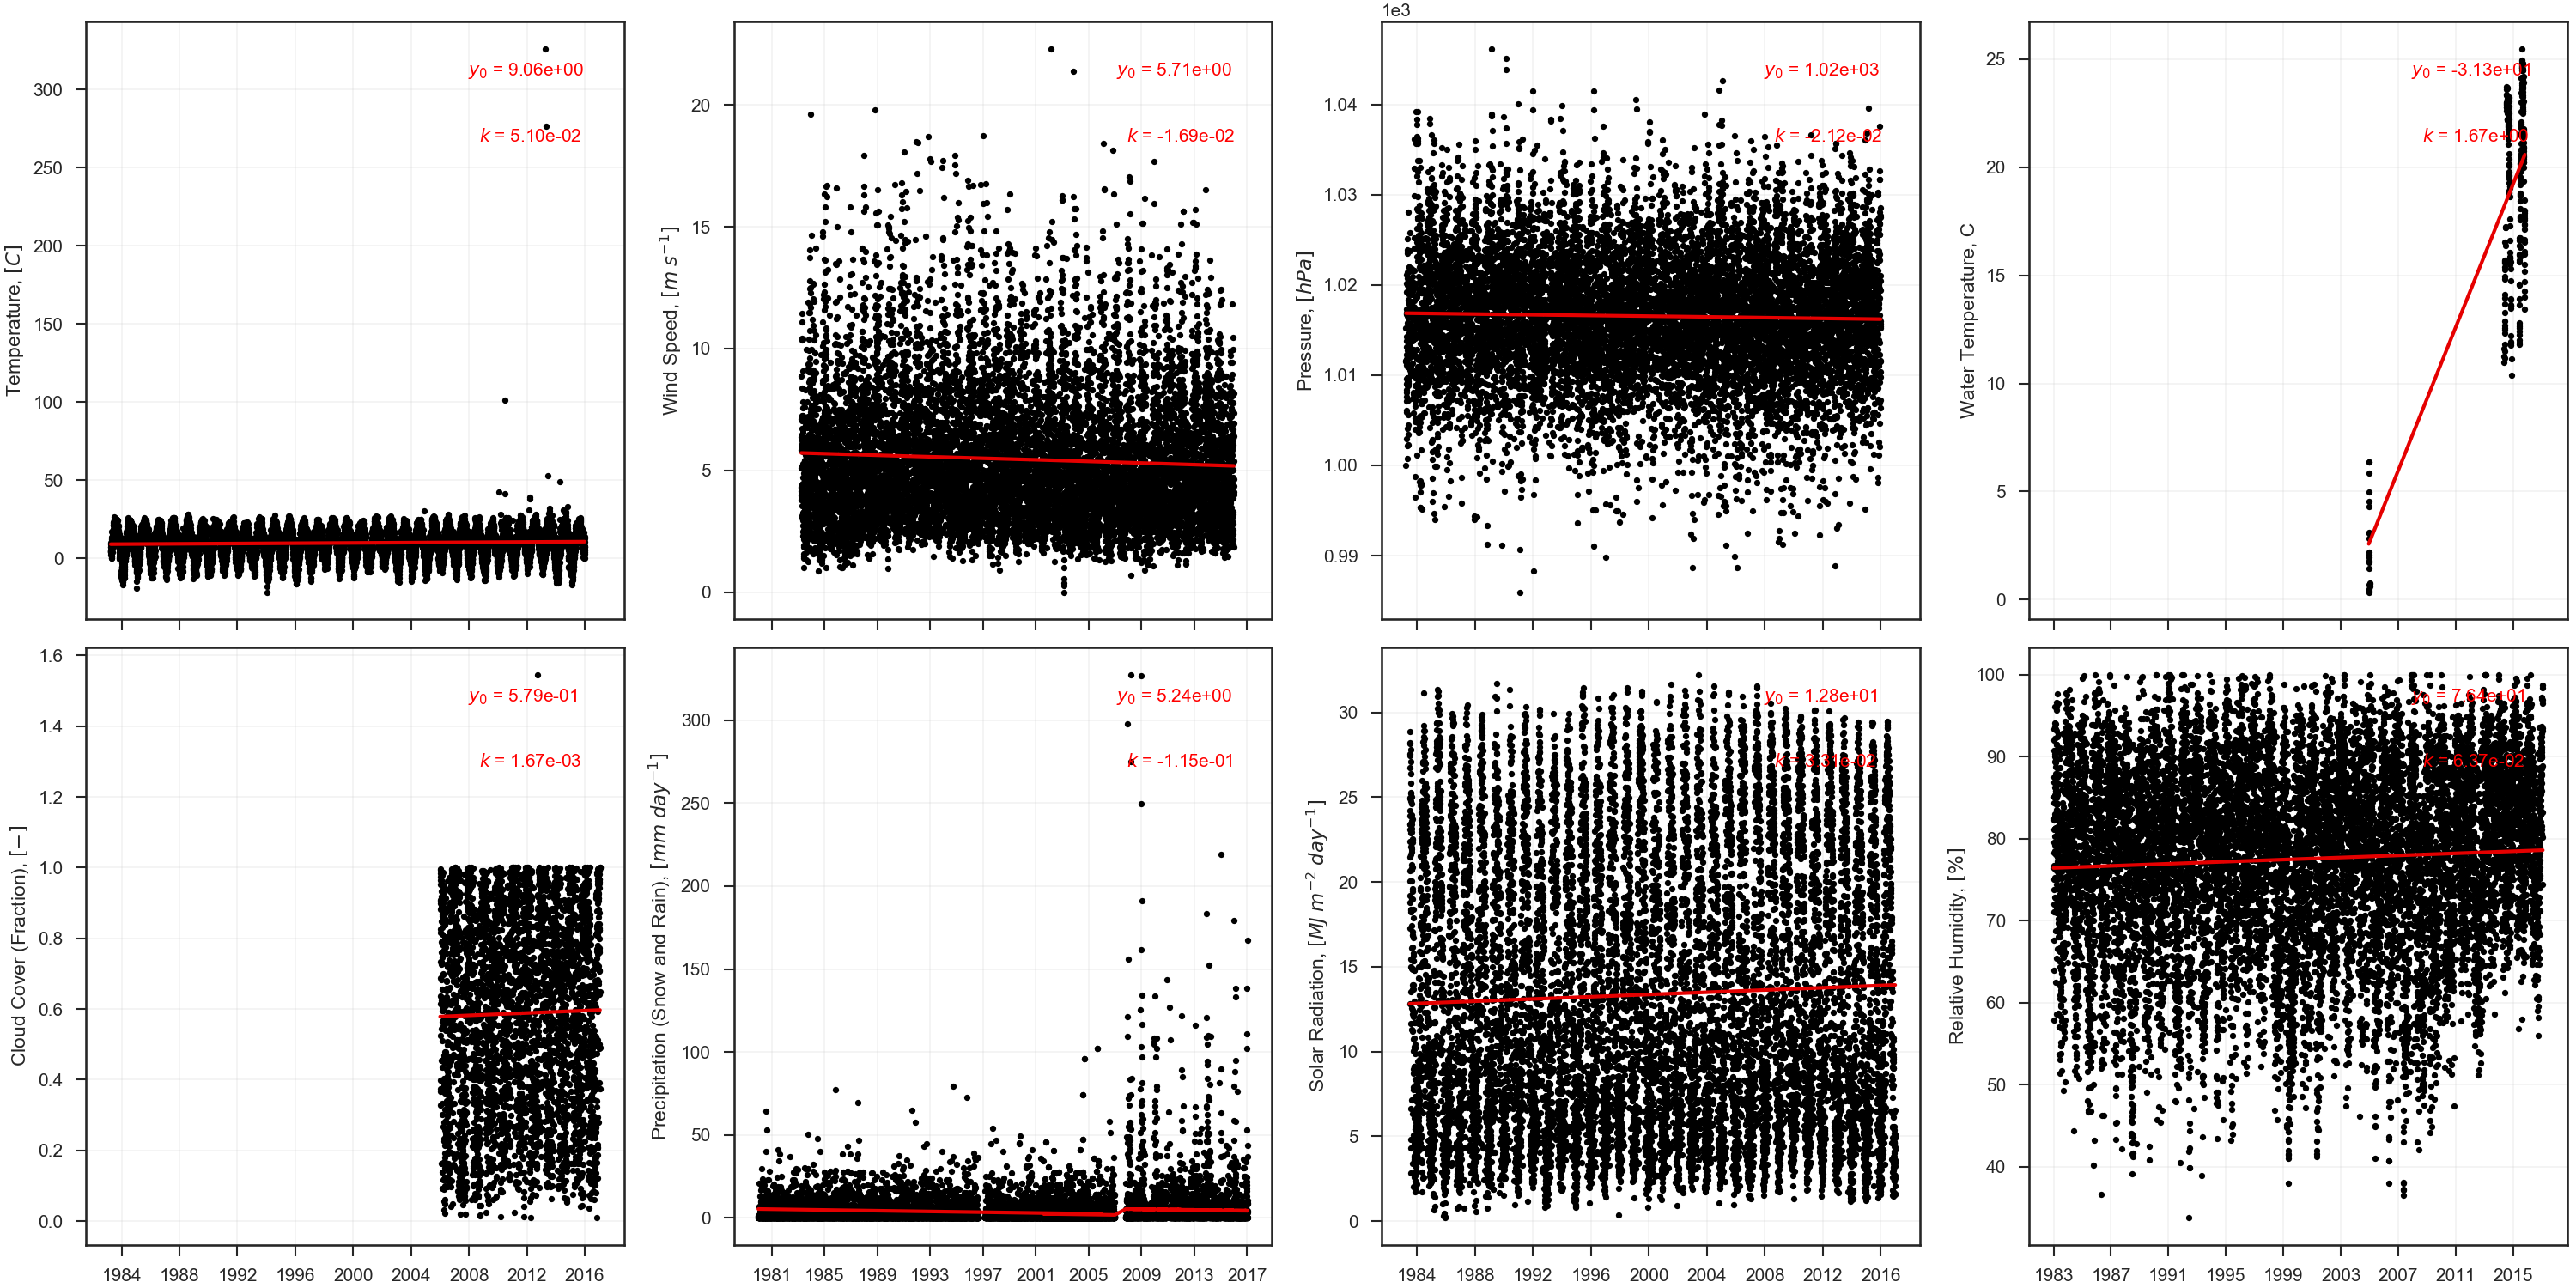
\includegraphics[width=\textwidth]{weather/eastern basin weather.png}
\end{figure}

\end{frame}

\section{US River Inputs}
\label{sec:river_inputs}

\subsection{Western Basin}
\label{sub:western_basin}

\begin{frame}
\frametitle{Western Basin: Detroit river}

\begin{figure}
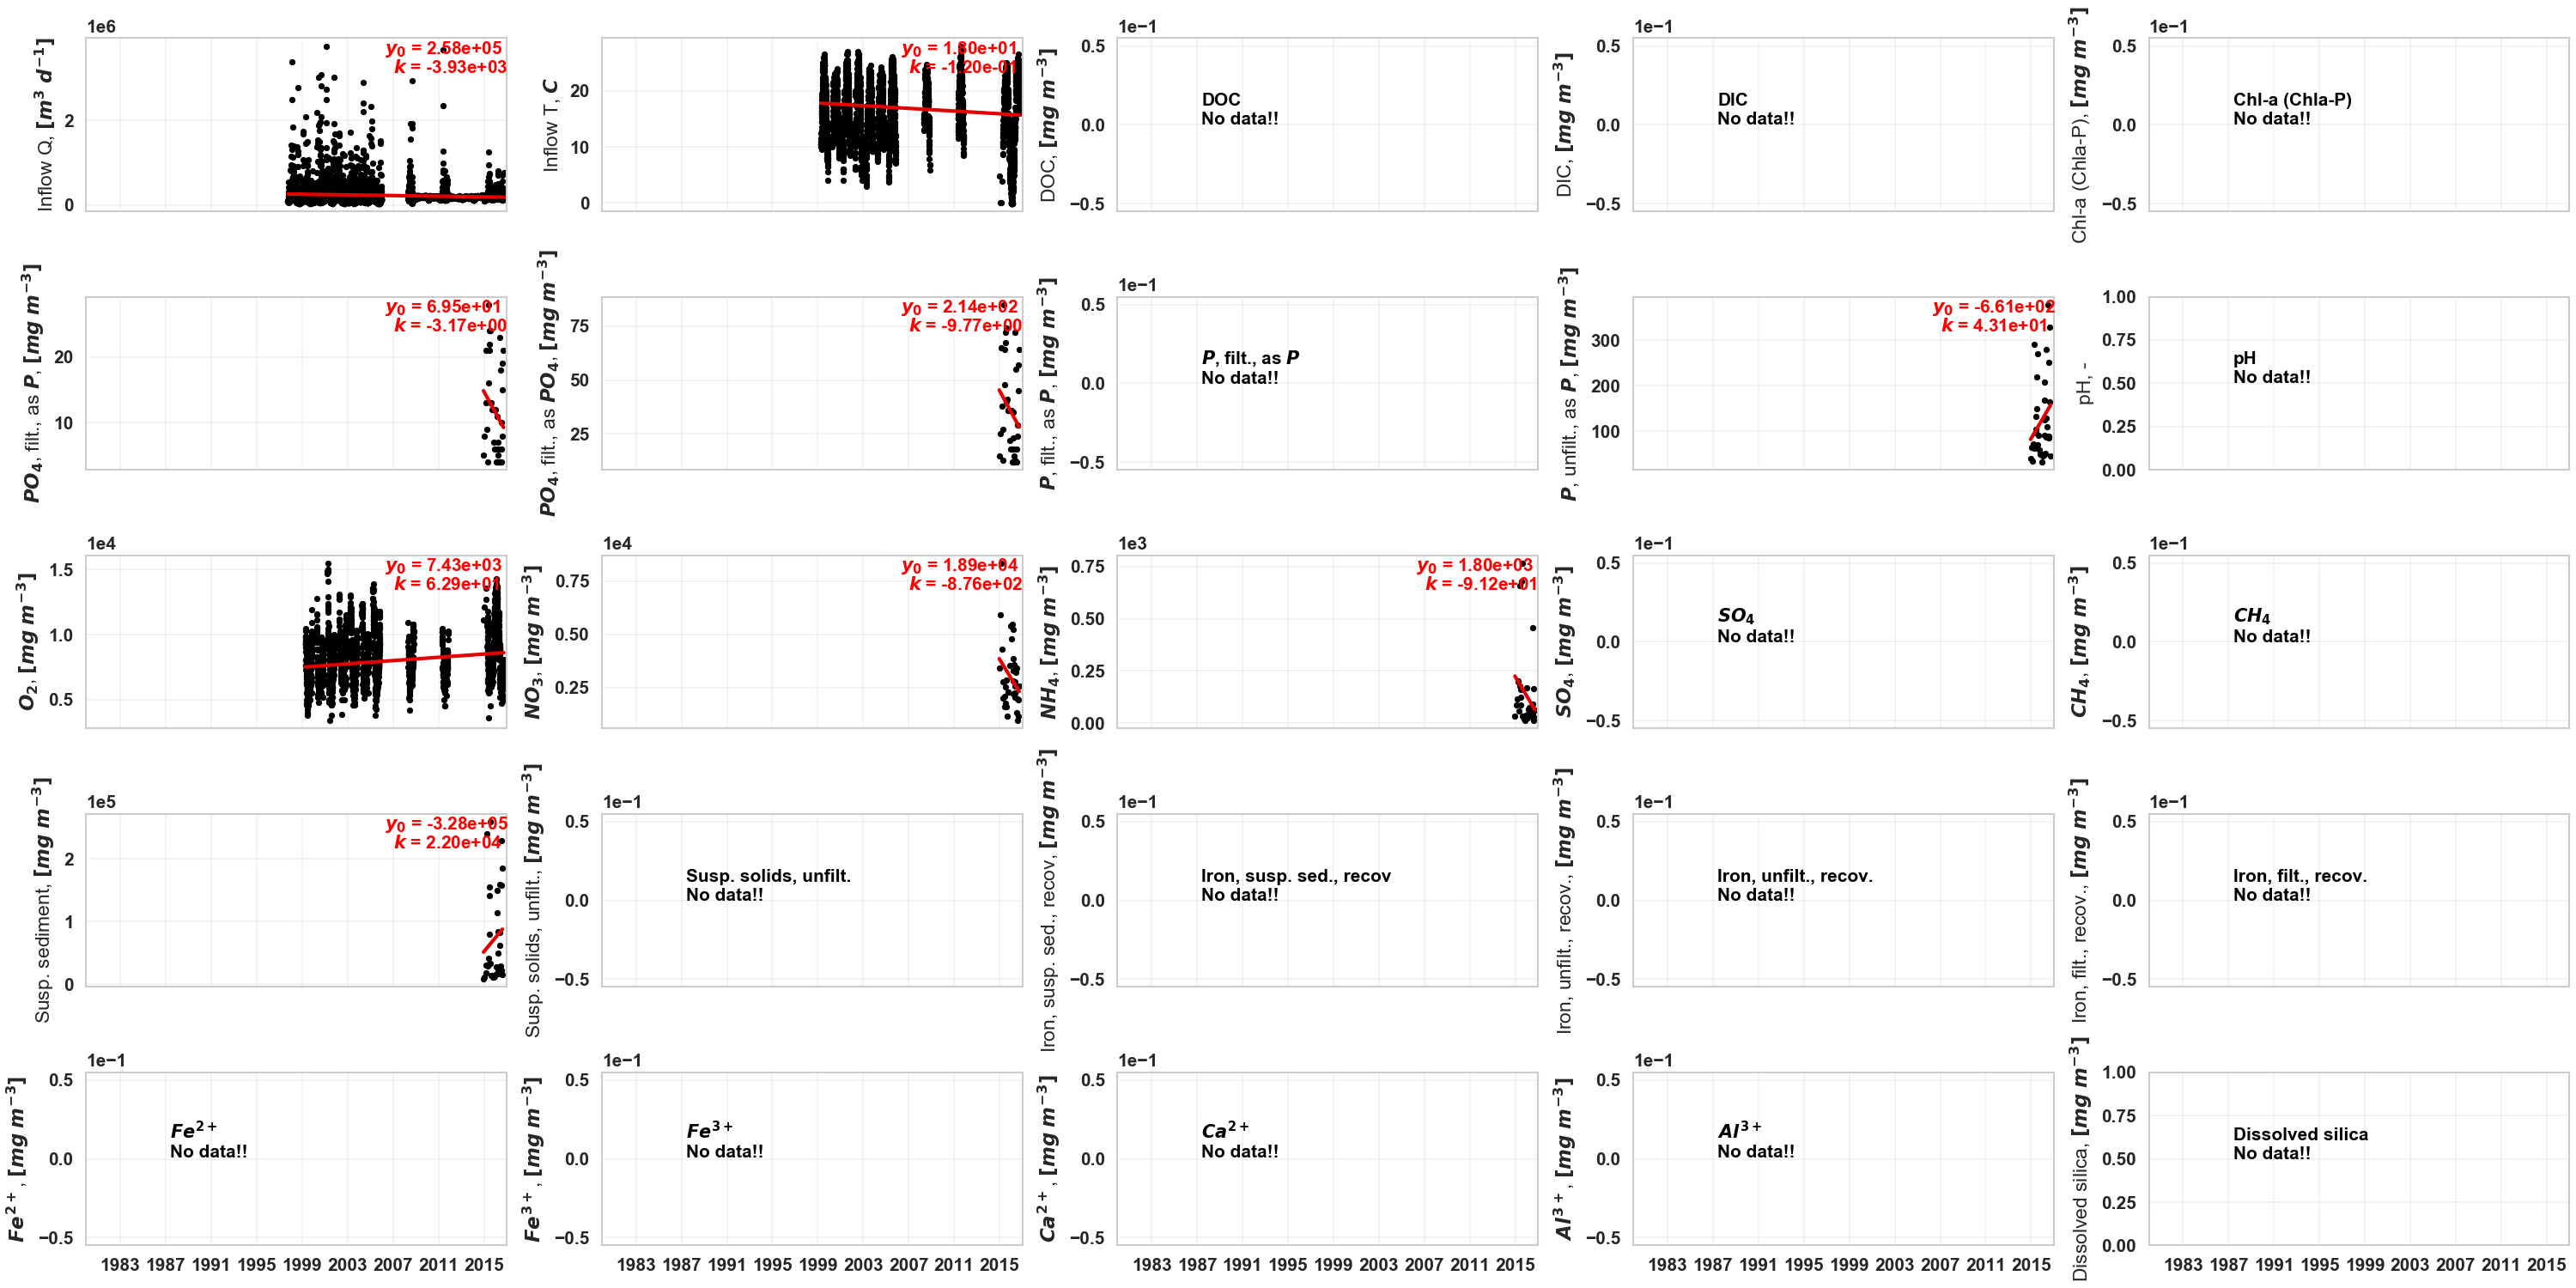
\includegraphics[width=\textwidth]{rivers/Western basin/detroitriver.png}
\end{figure}

\end{frame}


\begin{frame}
\frametitle{Western Basin: Huron river}

\begin{figure}
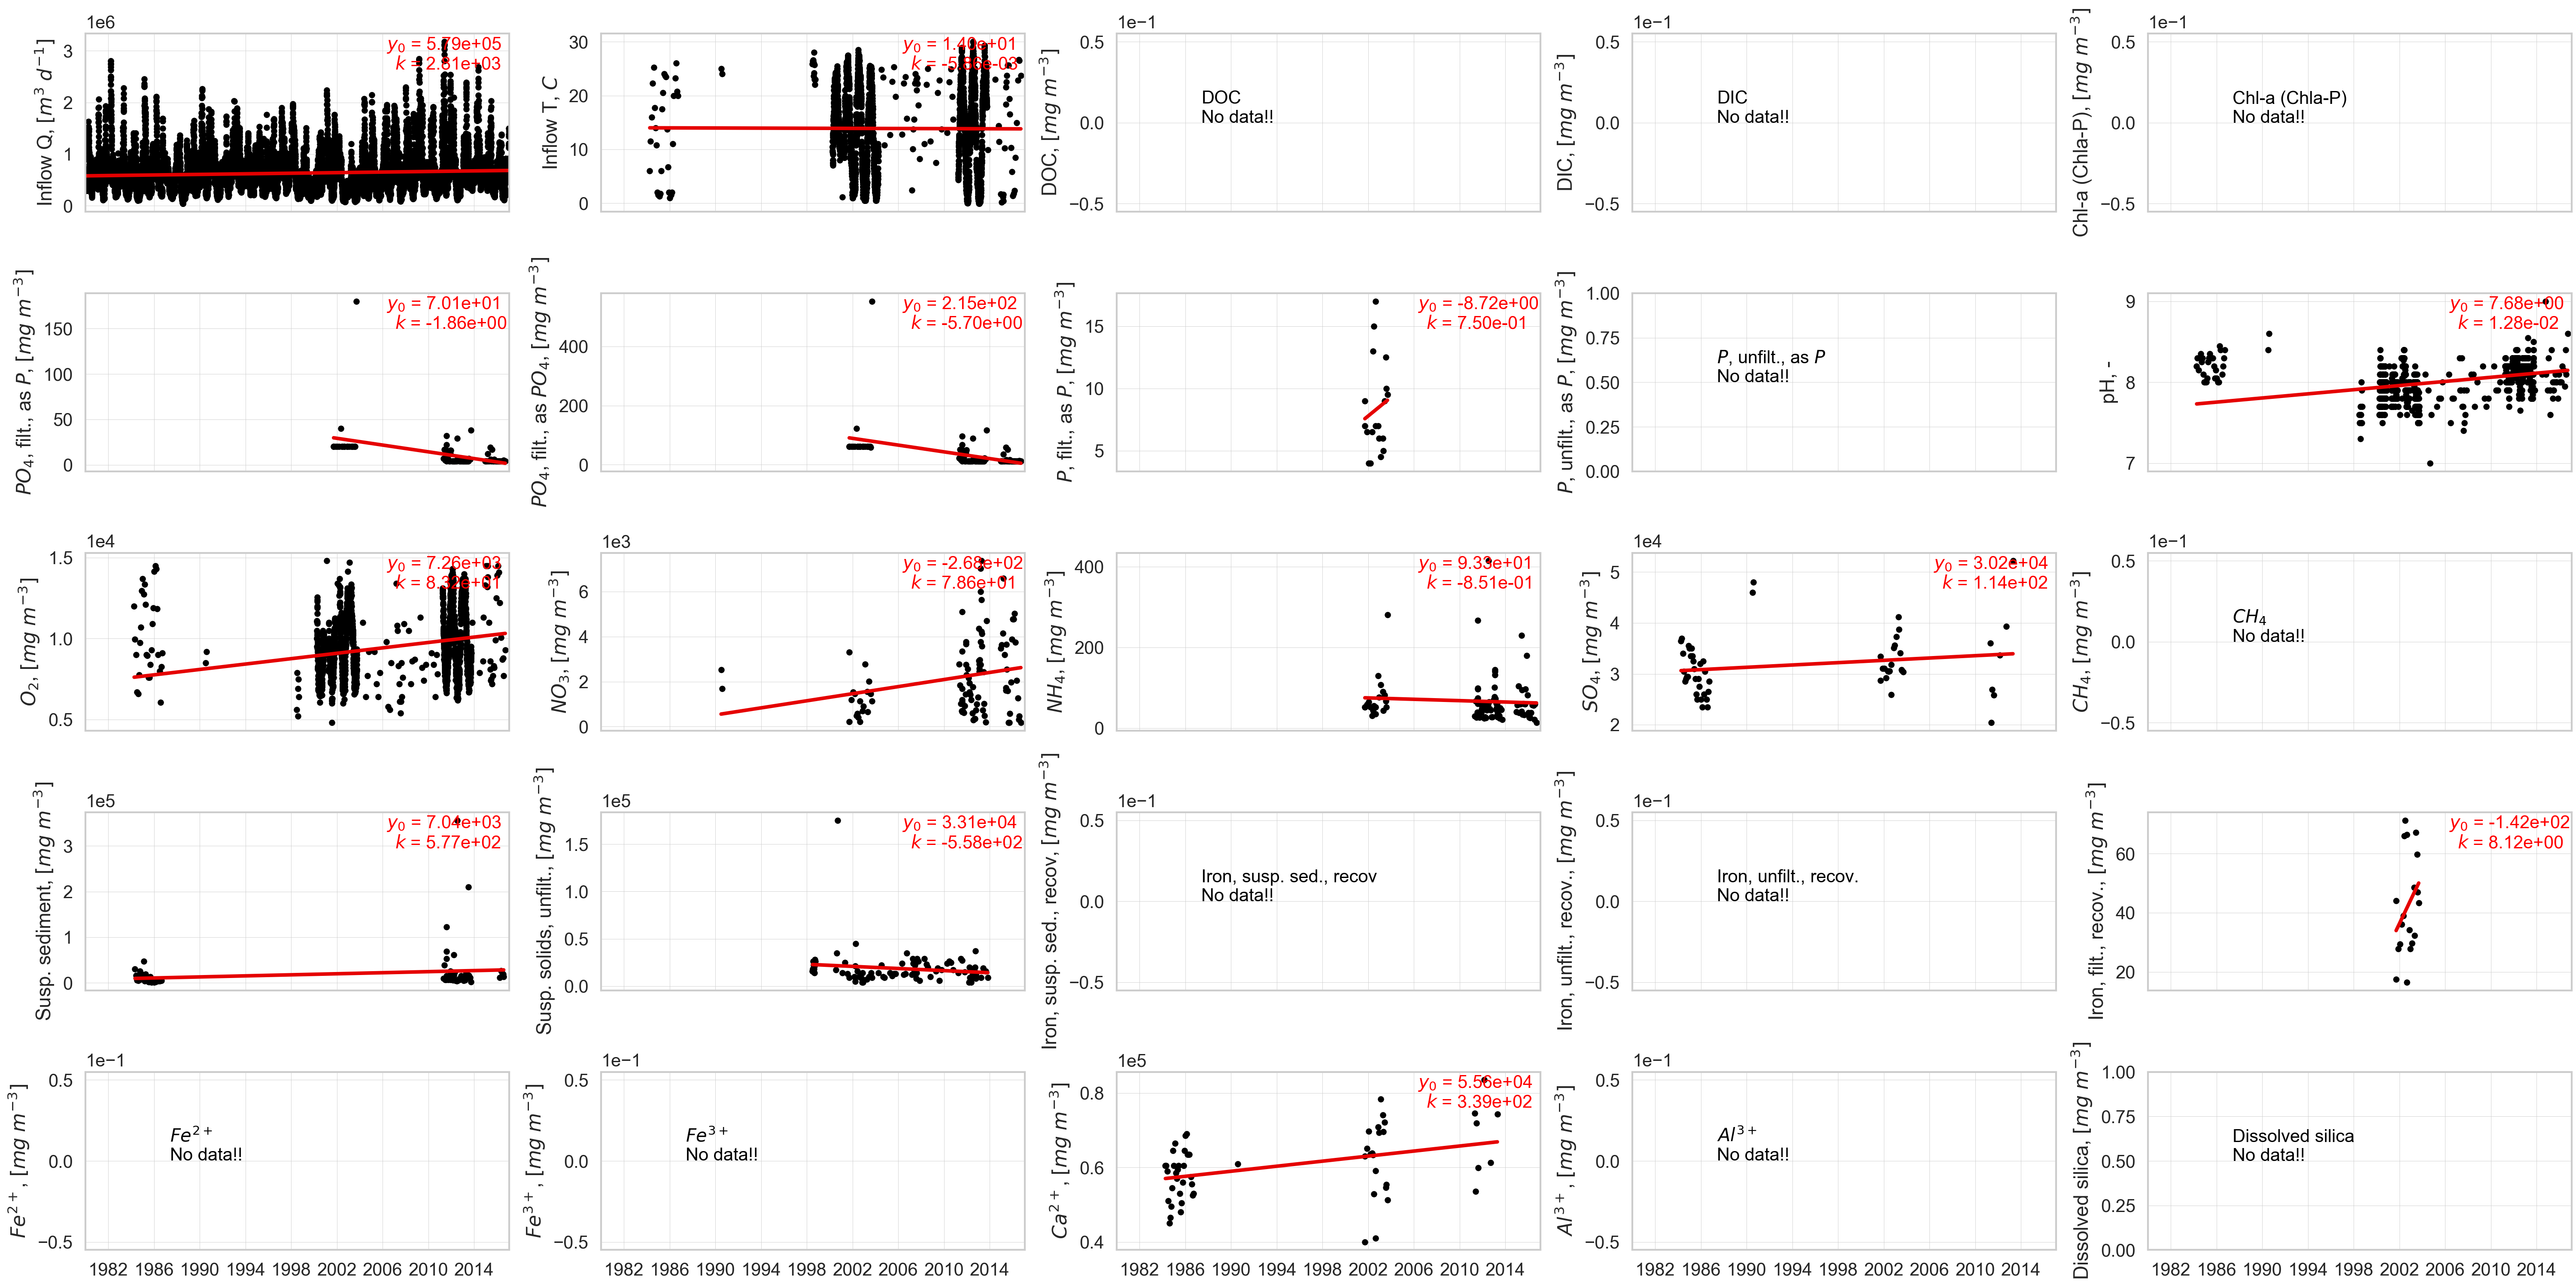
\includegraphics[width=\textwidth]{rivers/Western basin/huronriver.png}
\end{figure}

\end{frame}


\begin{frame}
\frametitle{Western Basin: Maumee river}

\begin{figure}
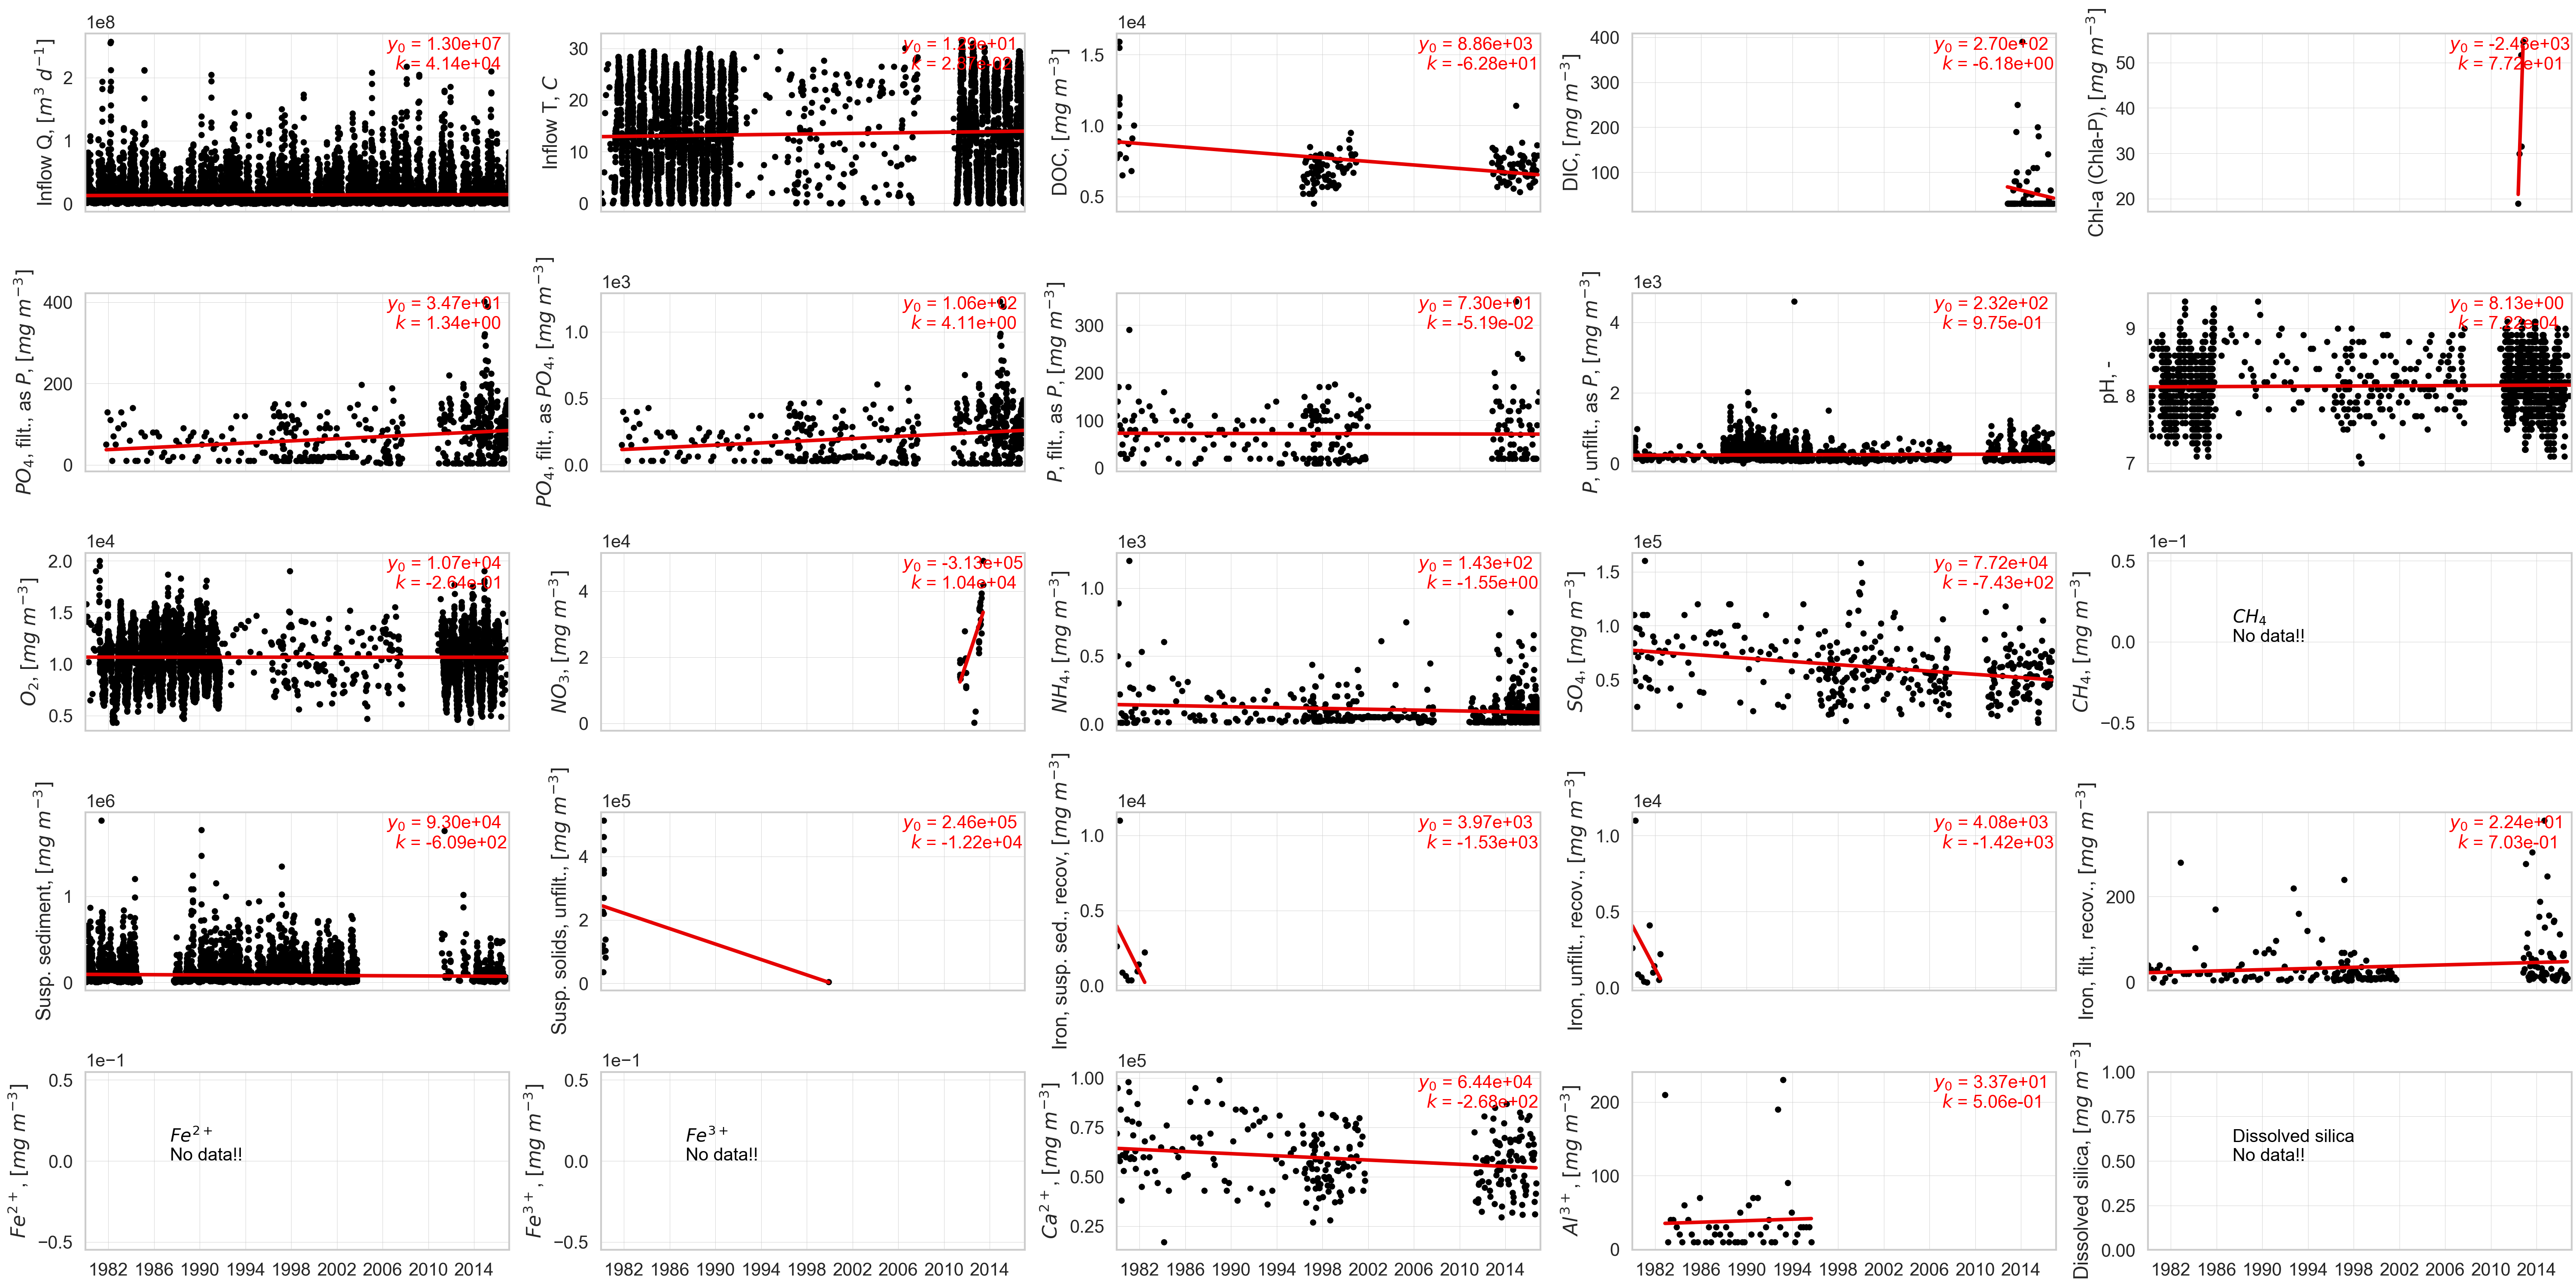
\includegraphics[width=\textwidth]{rivers/Western basin/maumeeriver.png}
\end{figure}

\end{frame}


\begin{frame}
\frametitle{Western Basin: Ottawa river}

\begin{figure}
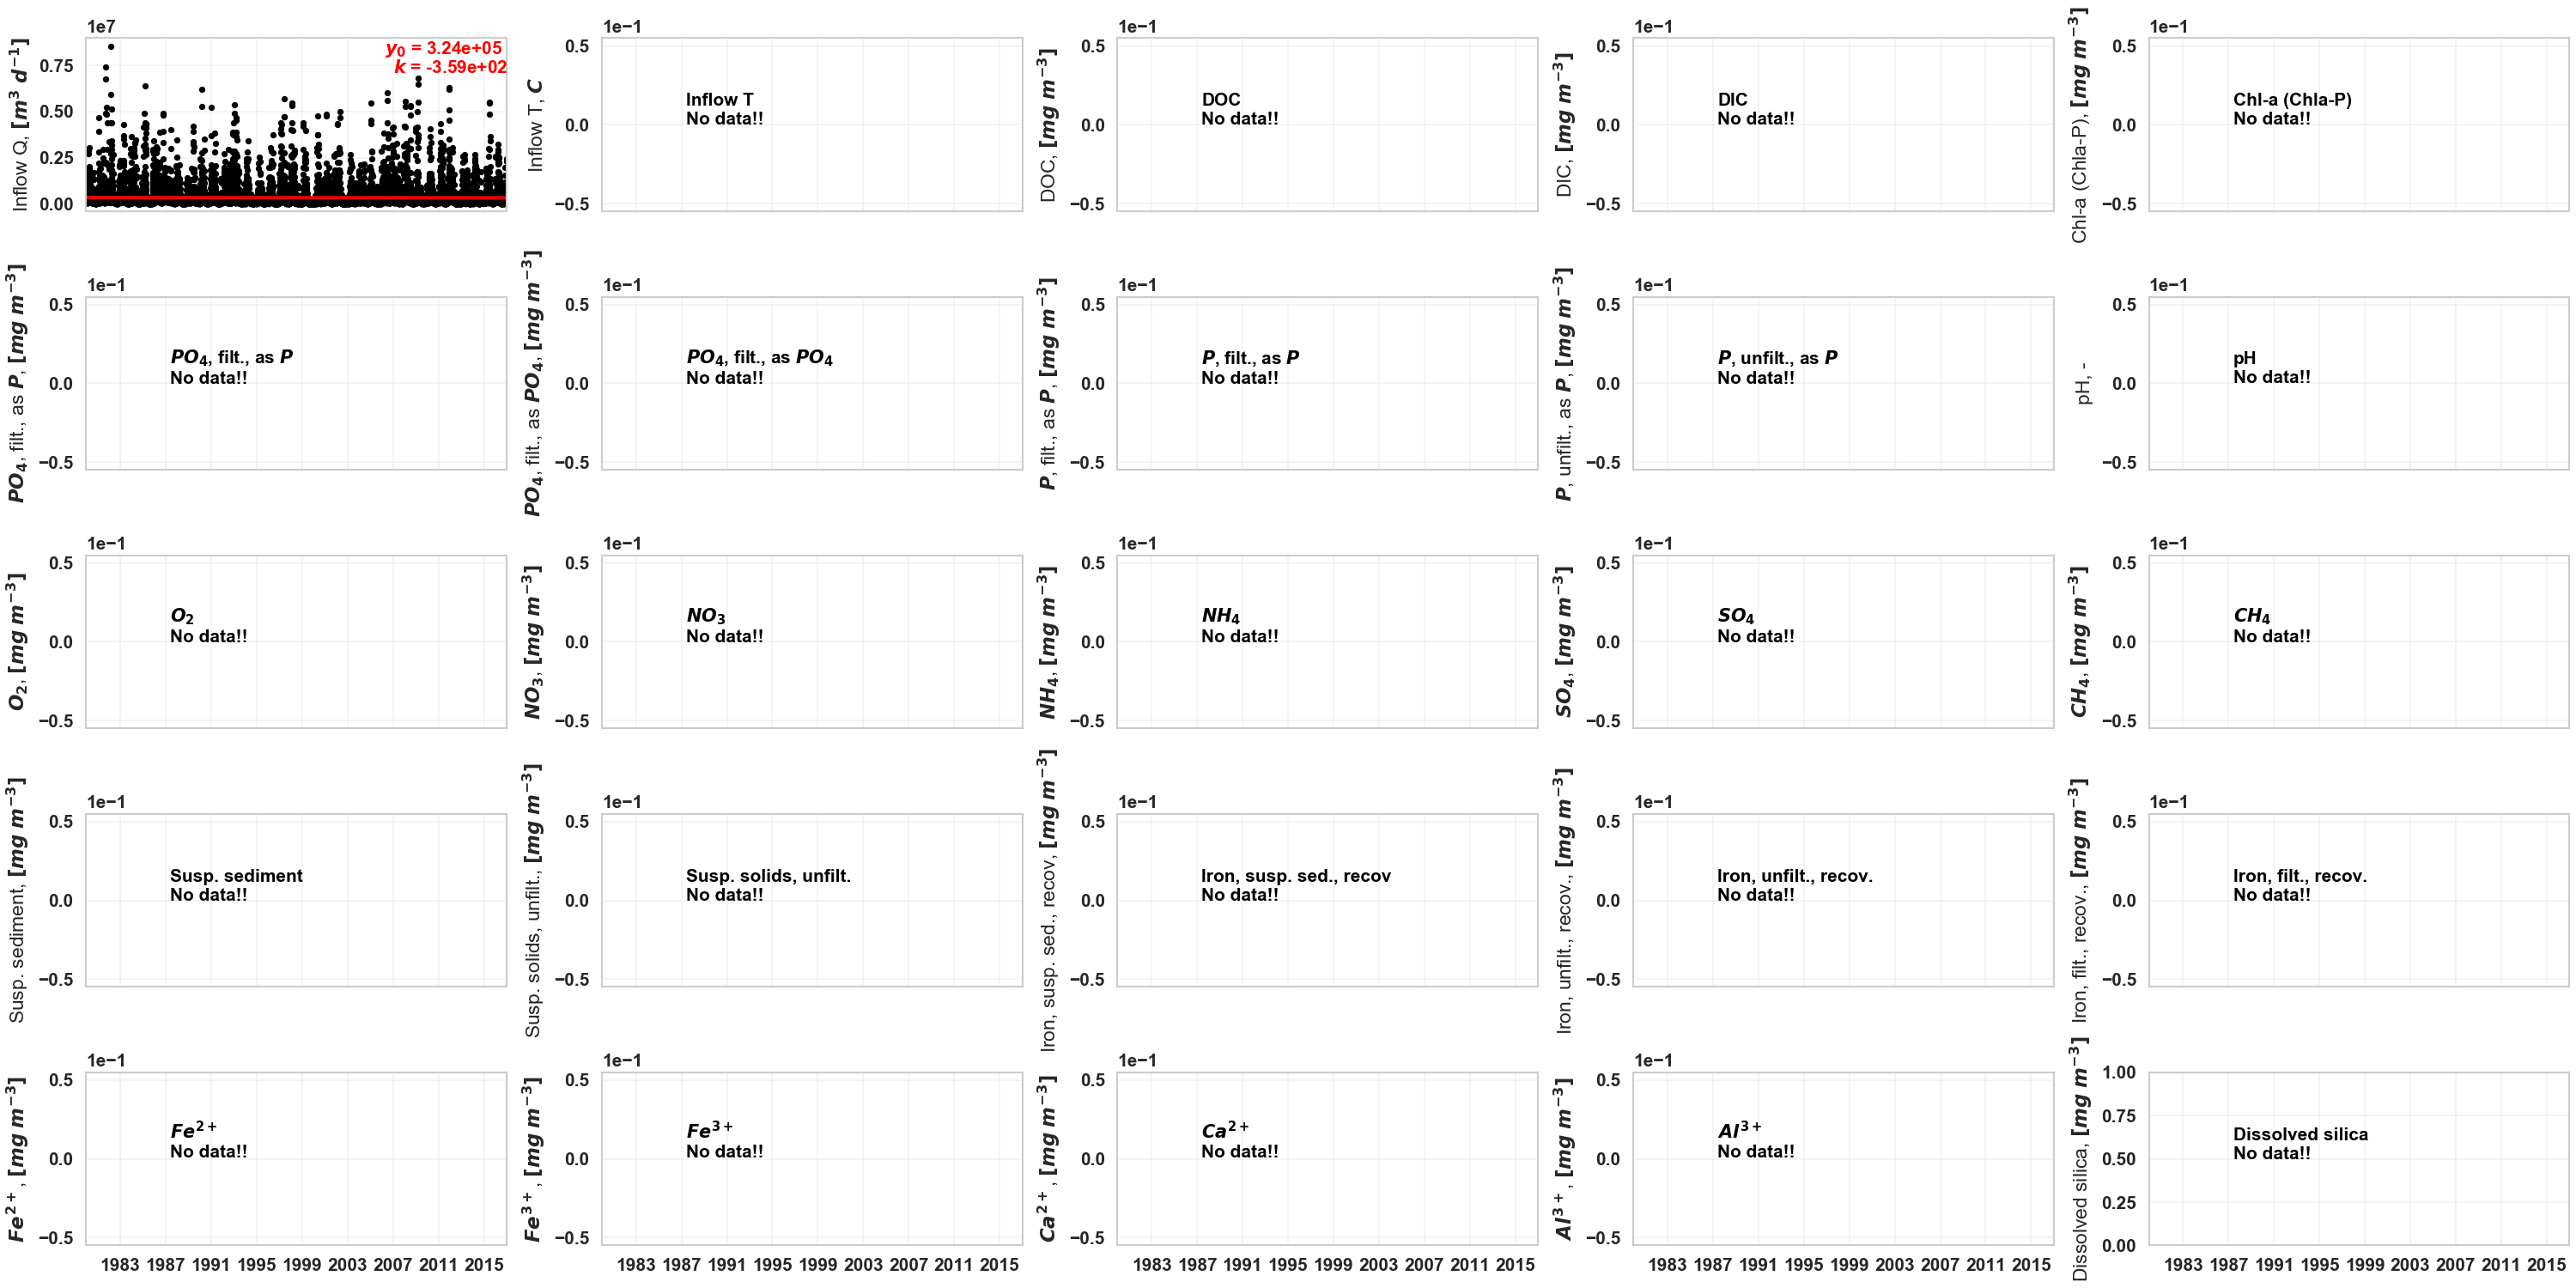
\includegraphics[width=\textwidth]{rivers/Western basin/ottawariver.png}
\end{figure}

\end{frame}


\begin{frame}
\frametitle{Western Basin: Portage river}

\begin{figure}
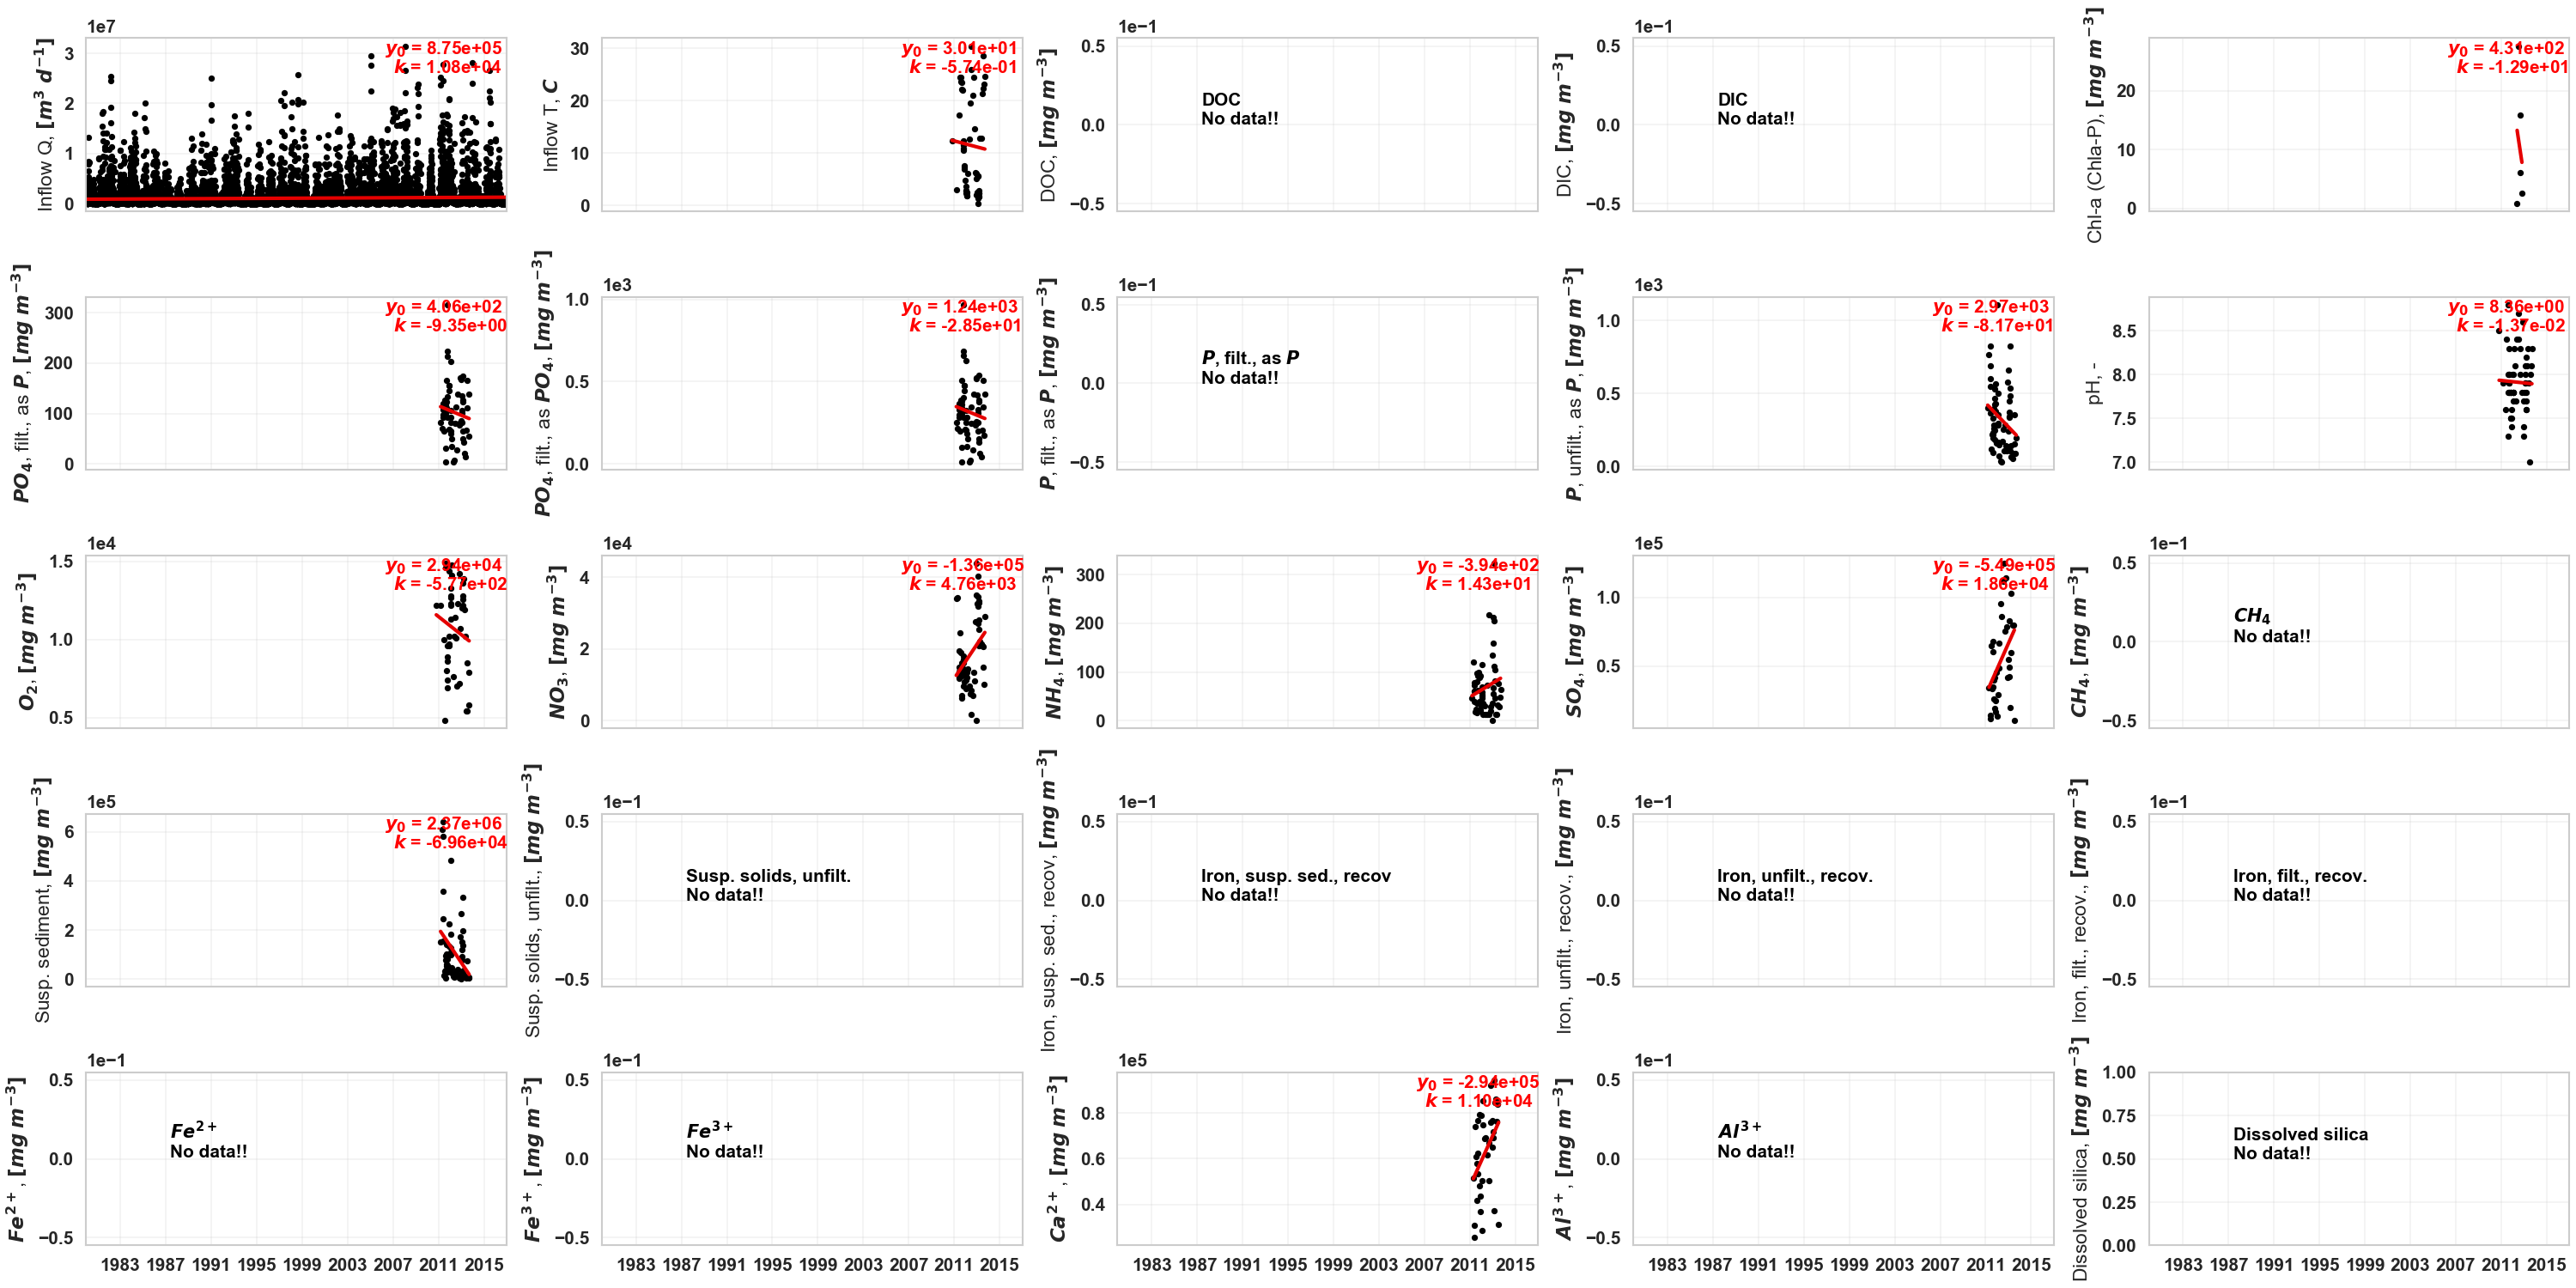
\includegraphics[width=\textwidth]{rivers/Western basin/portageriver.png}
\end{figure}

\end{frame}


\begin{frame}
\frametitle{Western Basin: Raisin river}

\begin{figure}
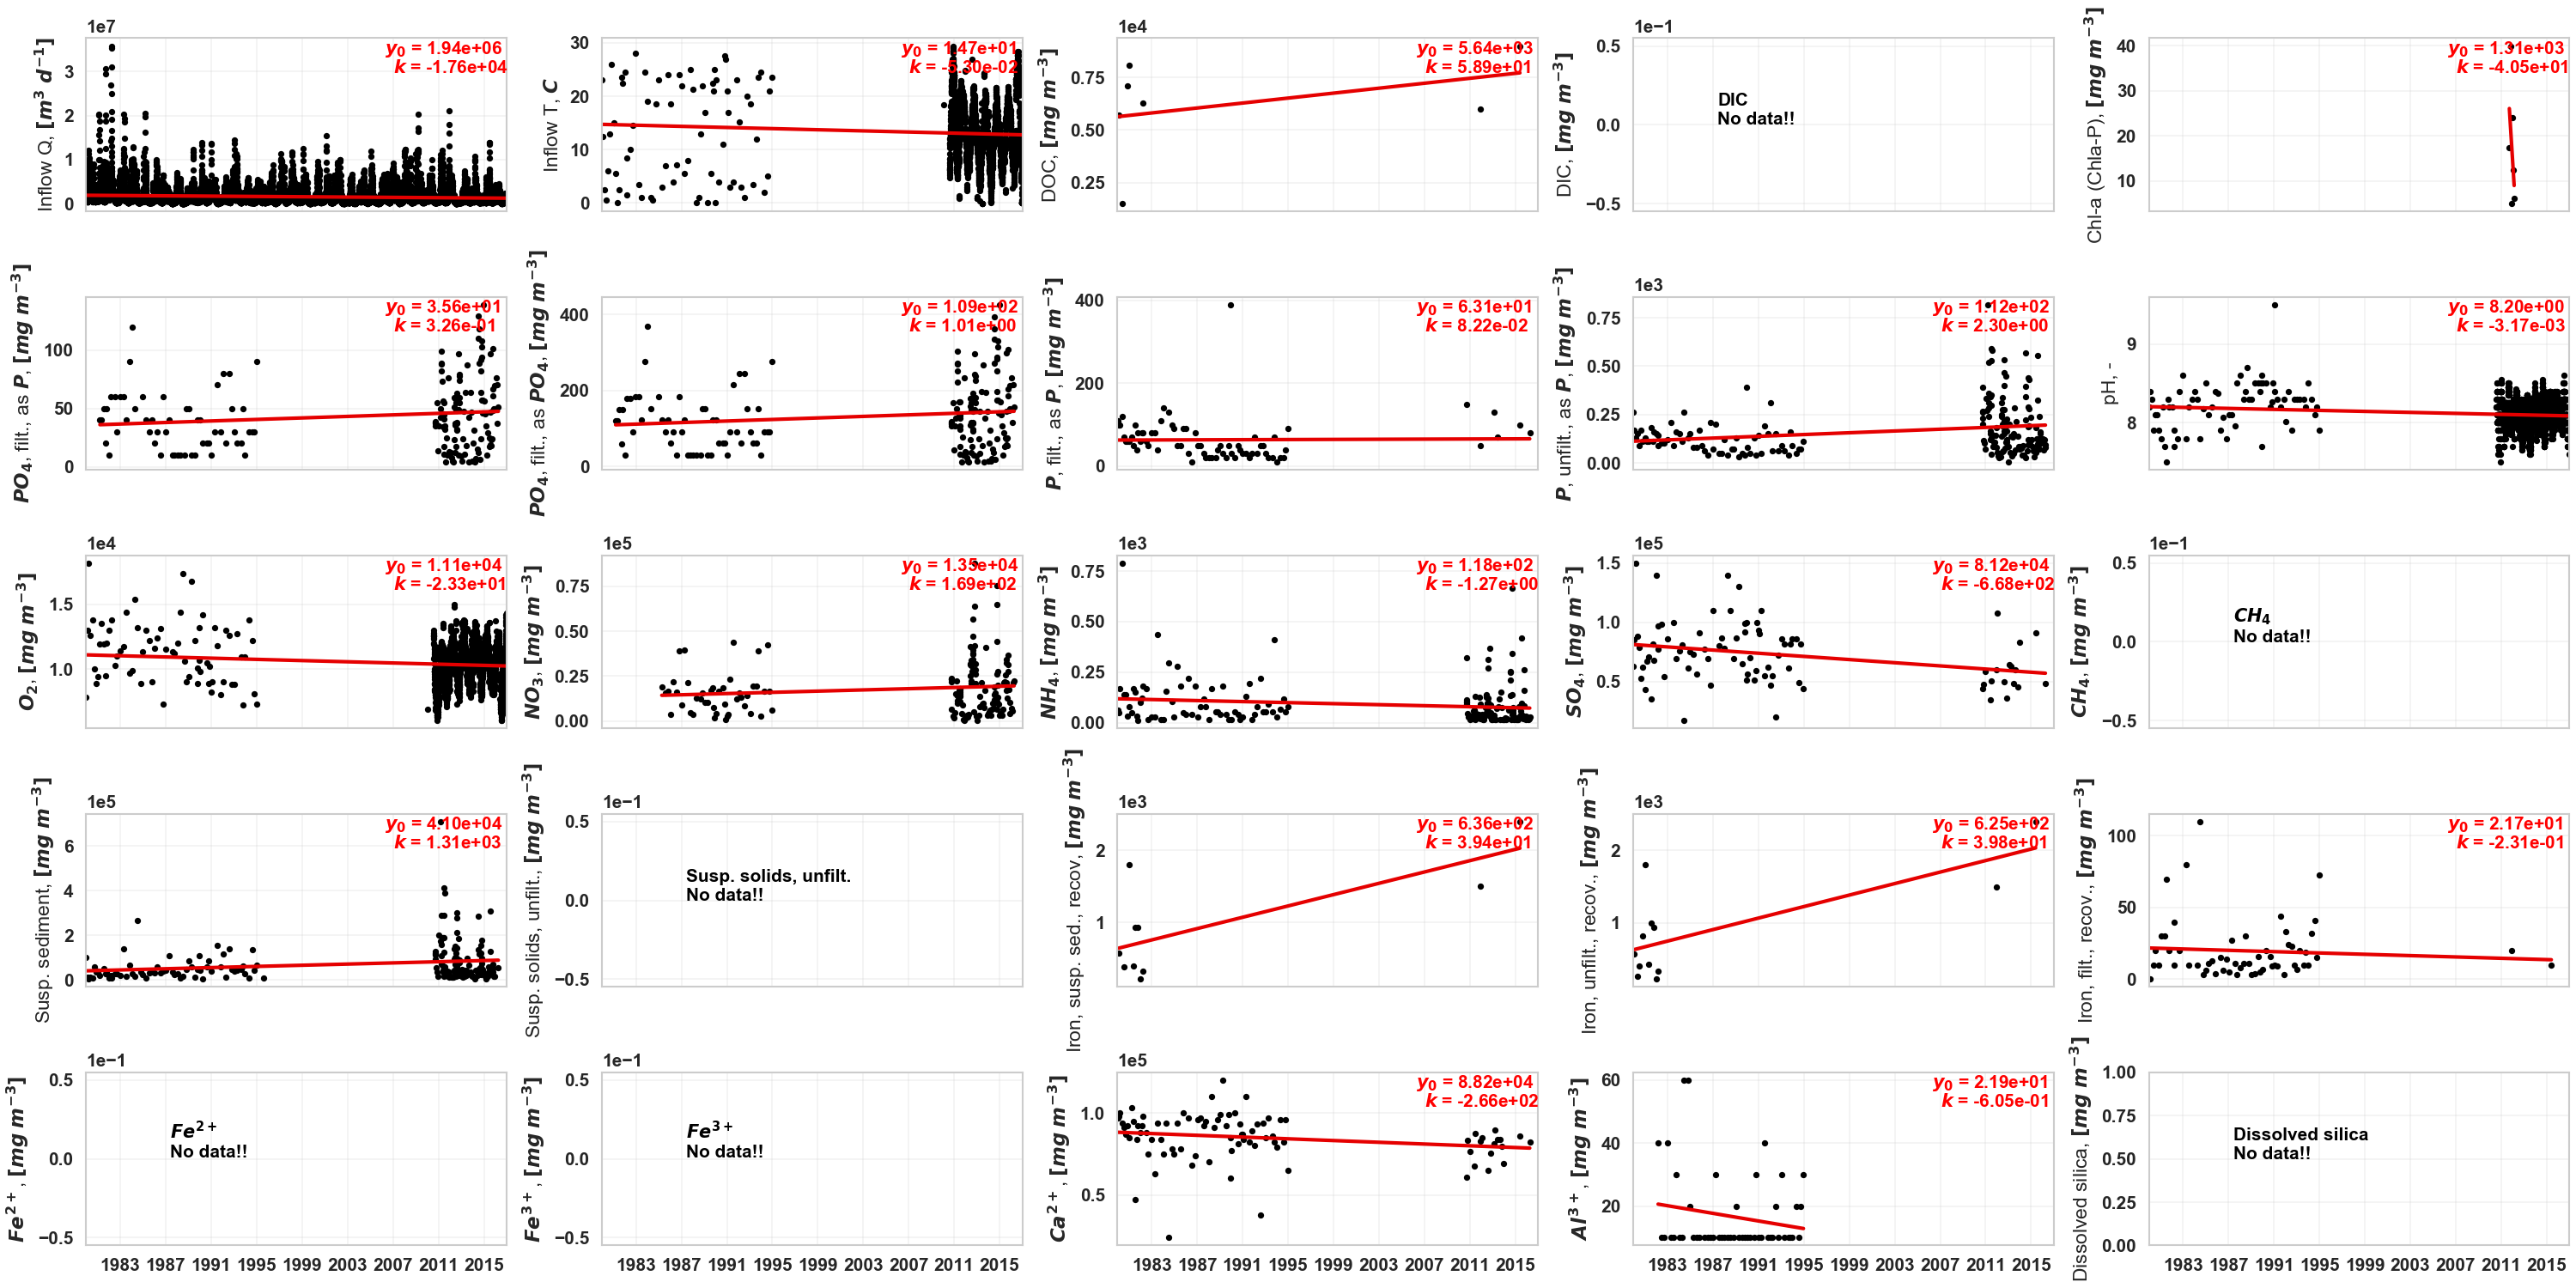
\includegraphics[width=\textwidth]{rivers/Western basin/riverraisin.png}
\end{figure}

\end{frame}


\begin{frame}
\frametitle{Western Basin: Stony creek}

\begin{figure}
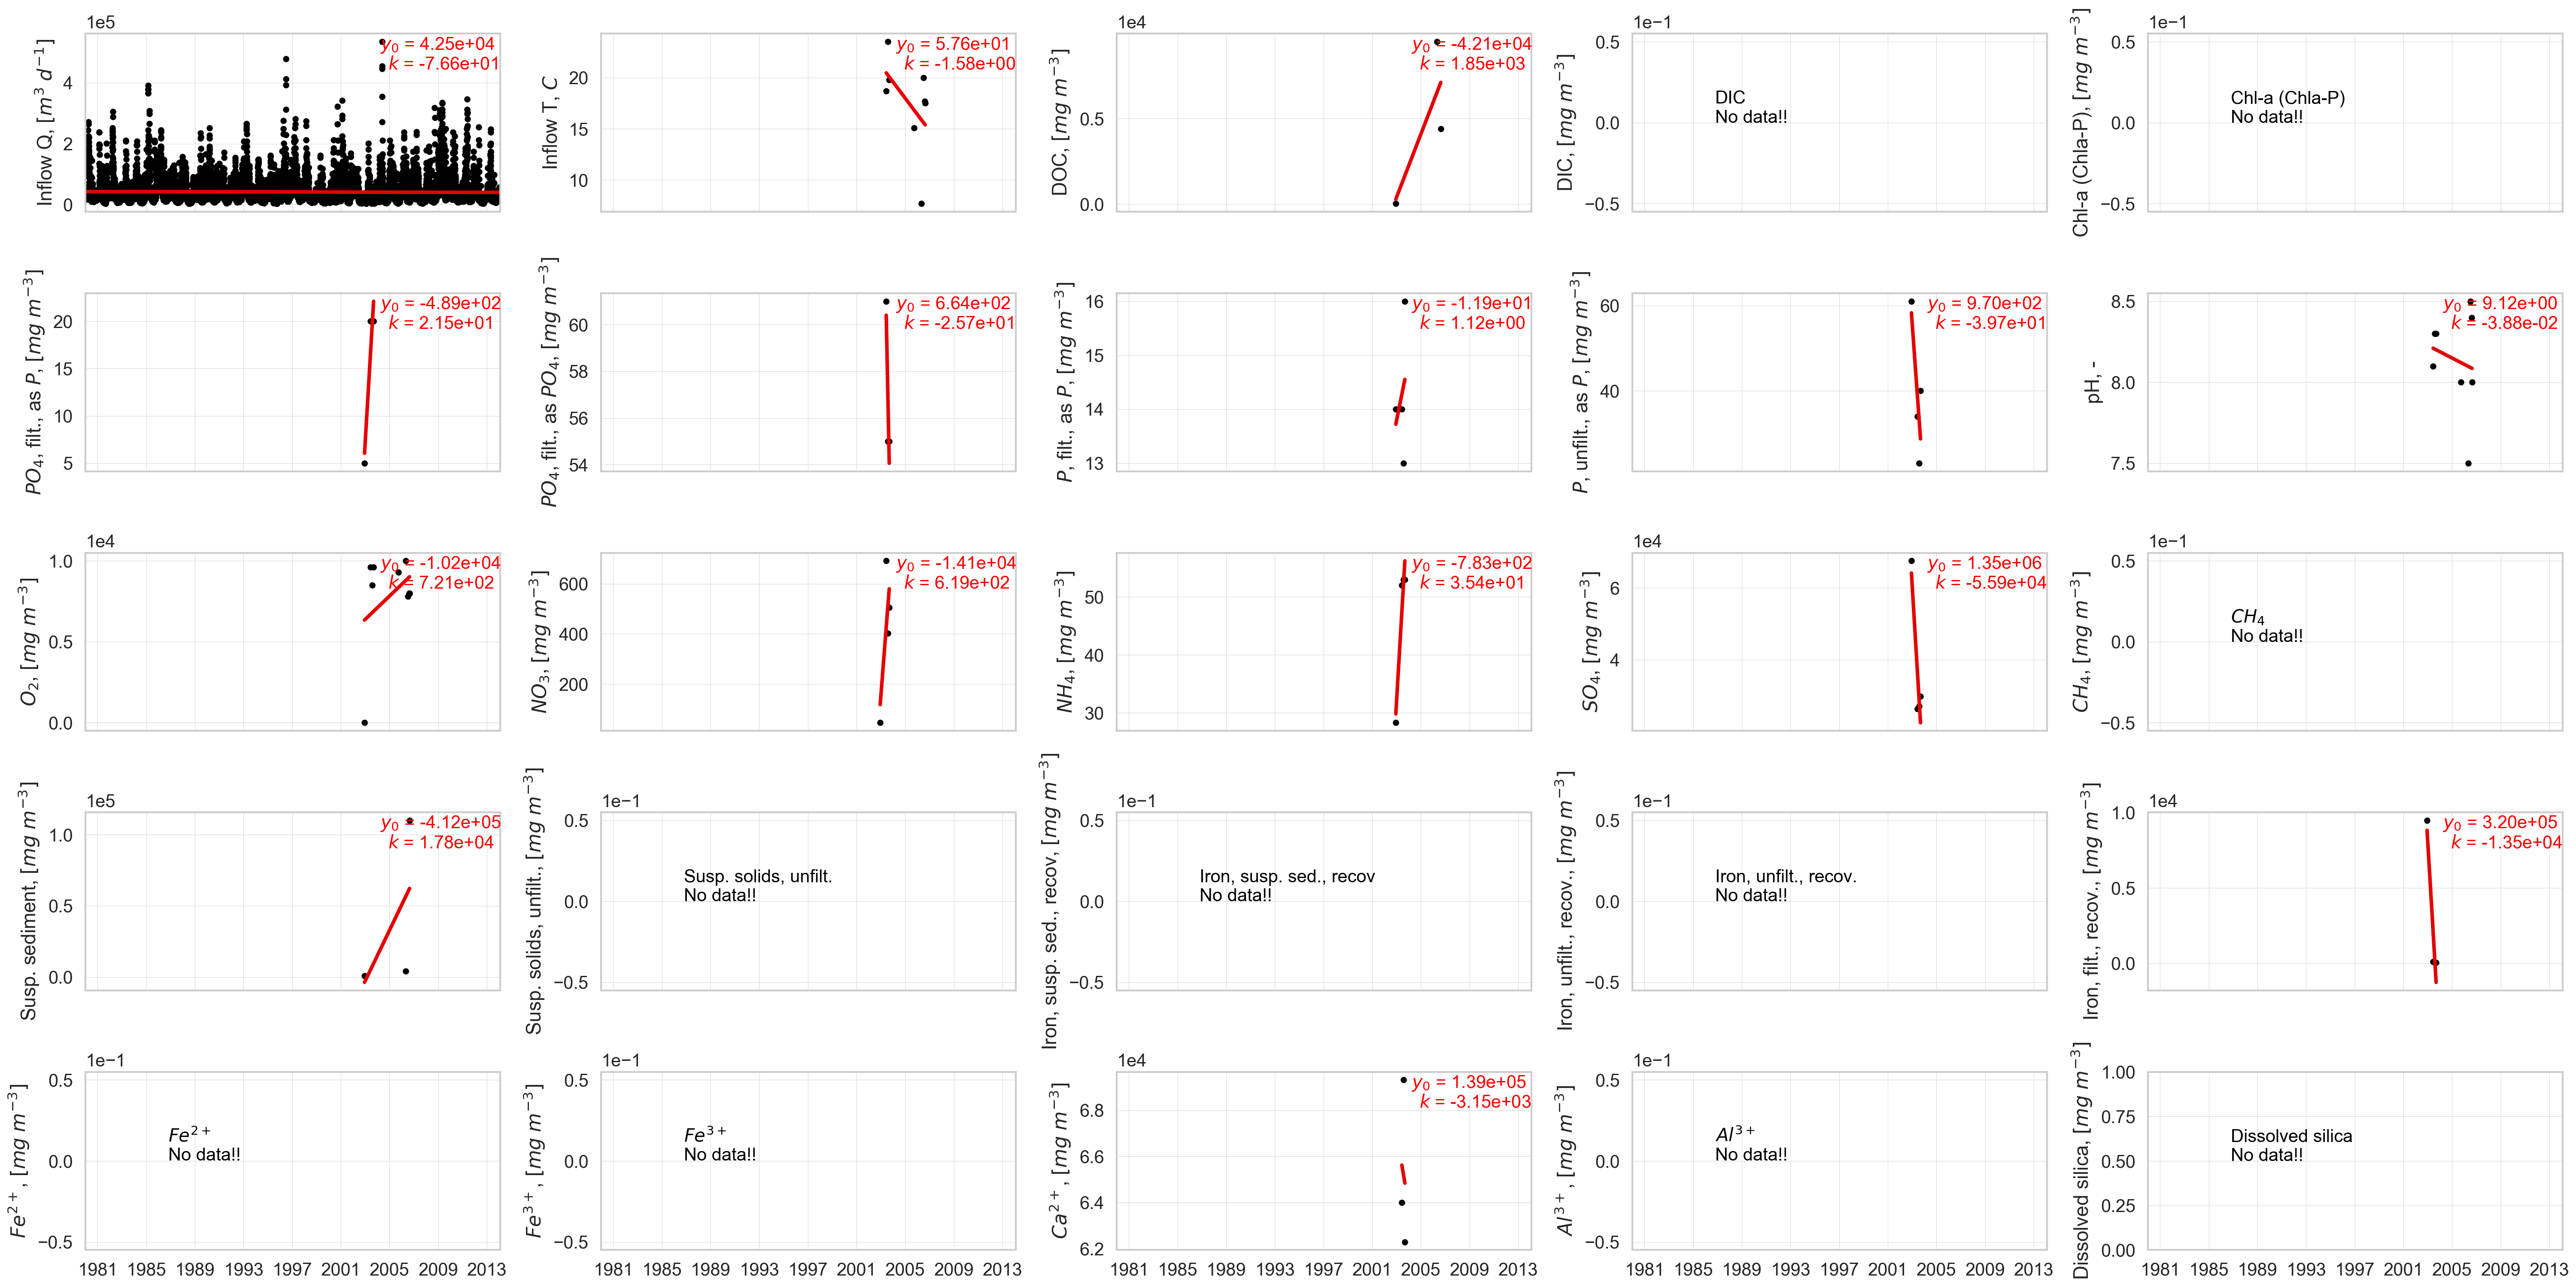
\includegraphics[width=\textwidth]{rivers/Western basin/stonycreek.png}
\end{figure}

\end{frame}


\begin{frame}
\frametitle{Western Basin: Swan creek}

\begin{figure}
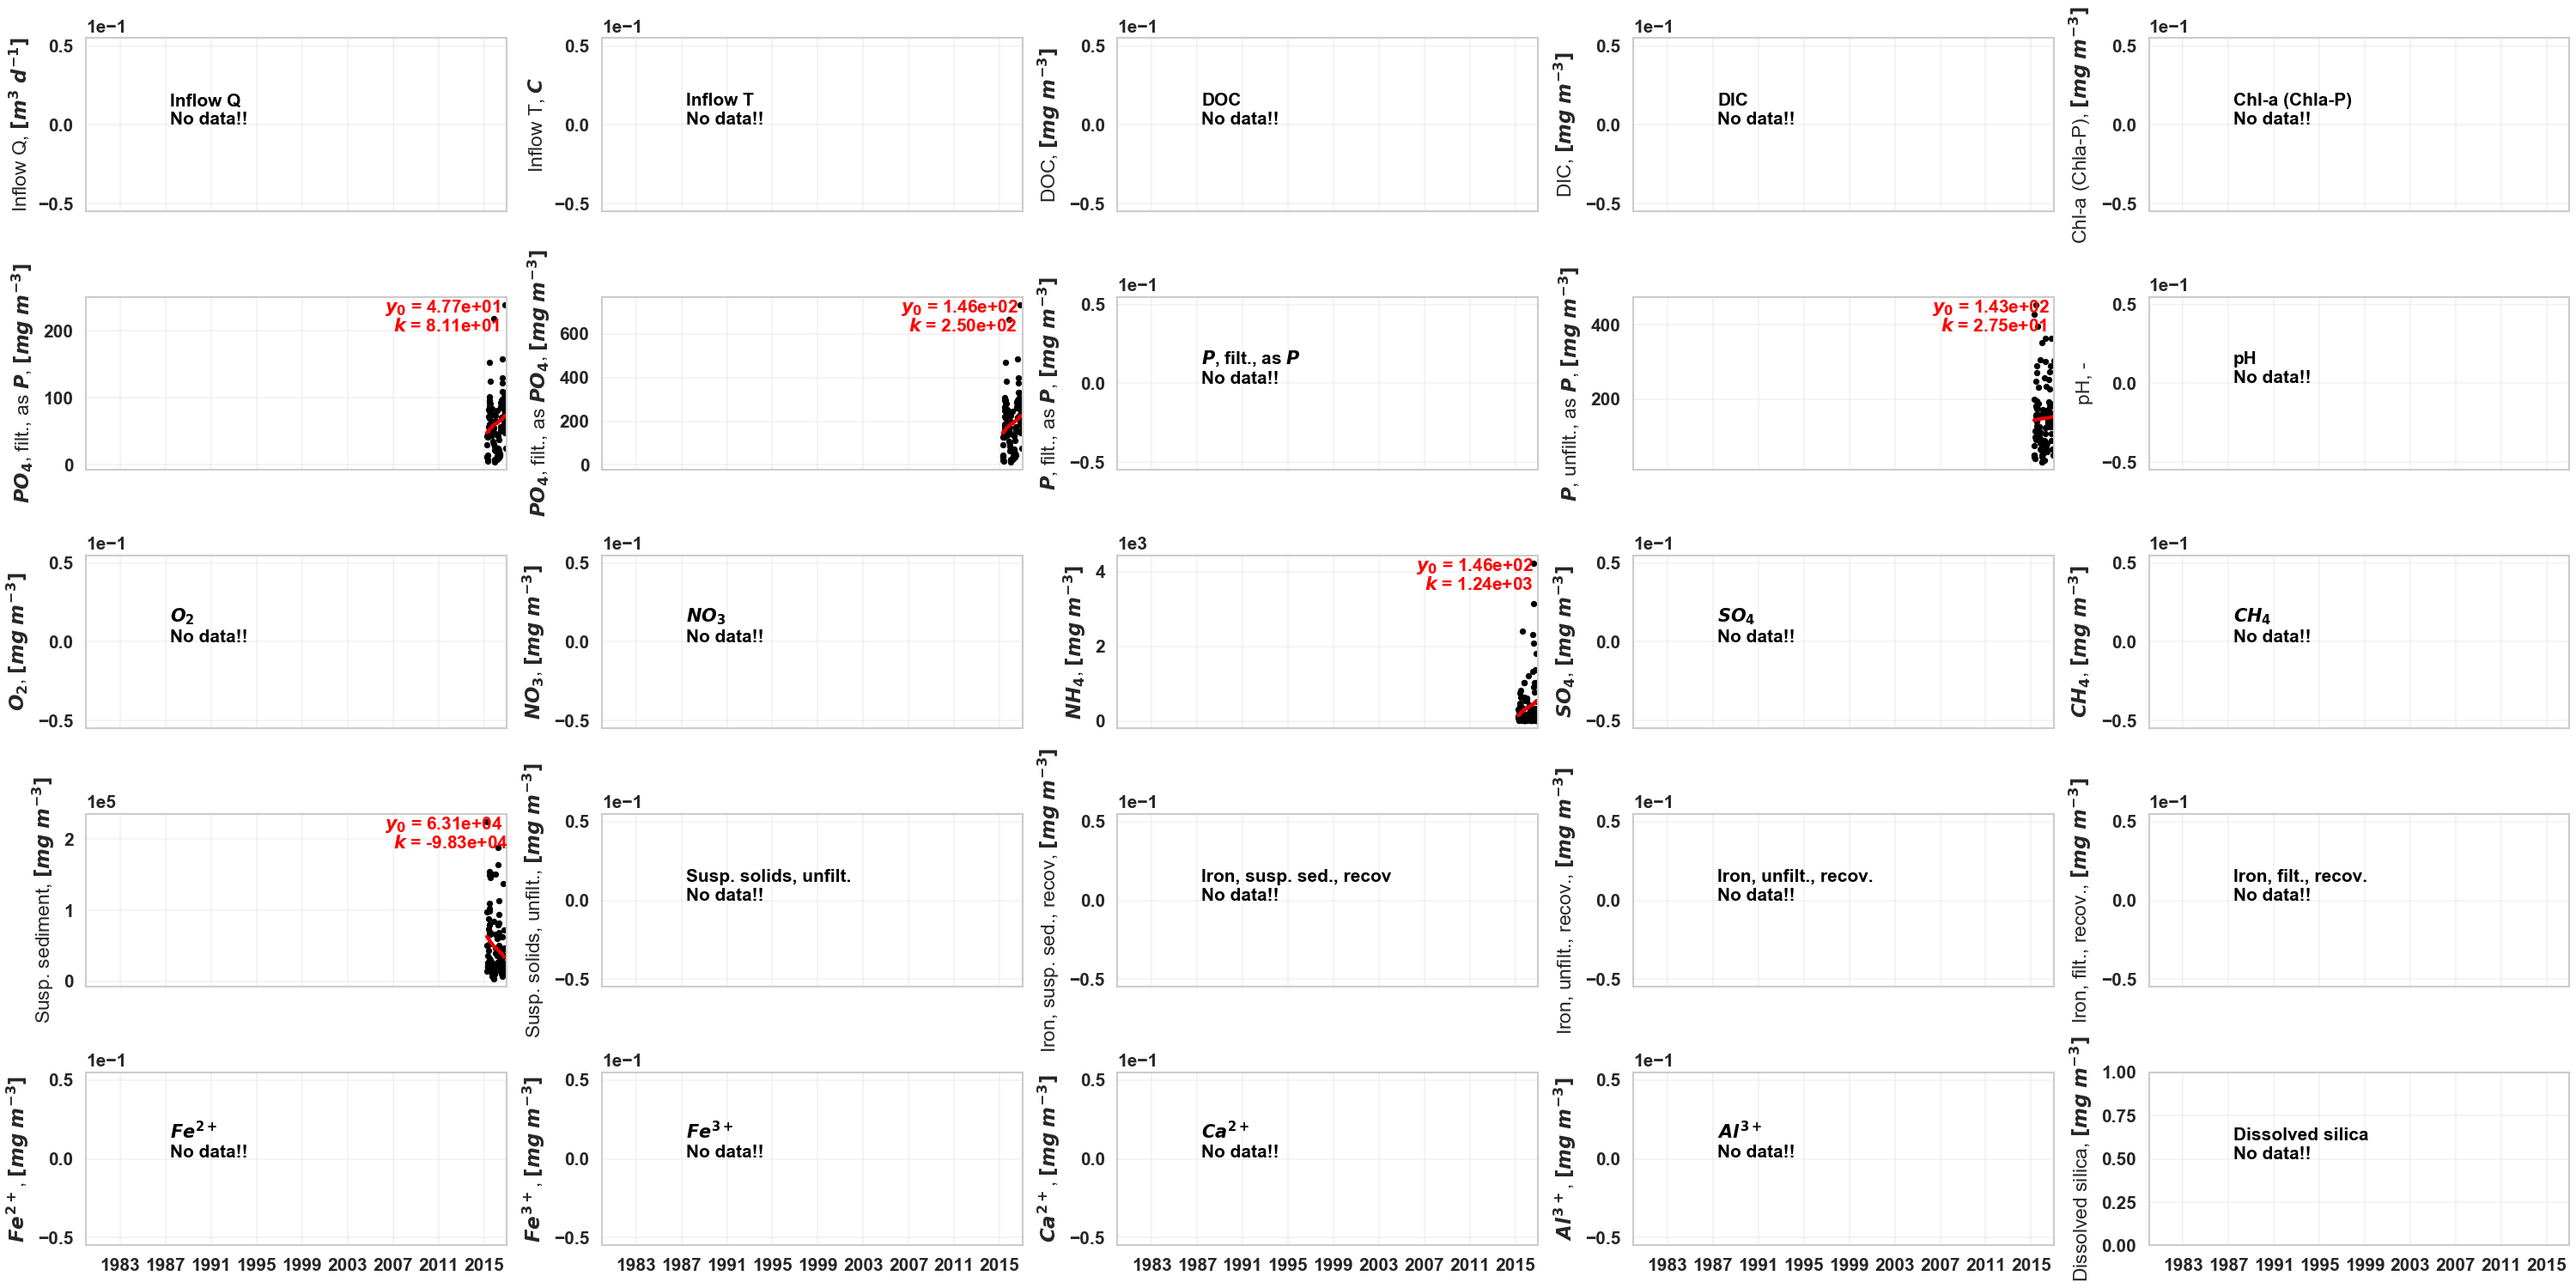
\includegraphics[width=\textwidth]{rivers/Western basin/swancreek.png}
\end{figure}

\end{frame}



\subsection{Central Basin}
\label{sub:central_basin}


\begin{frame}
\frametitle{Central Basin: Ashtabula river}

\begin{figure}
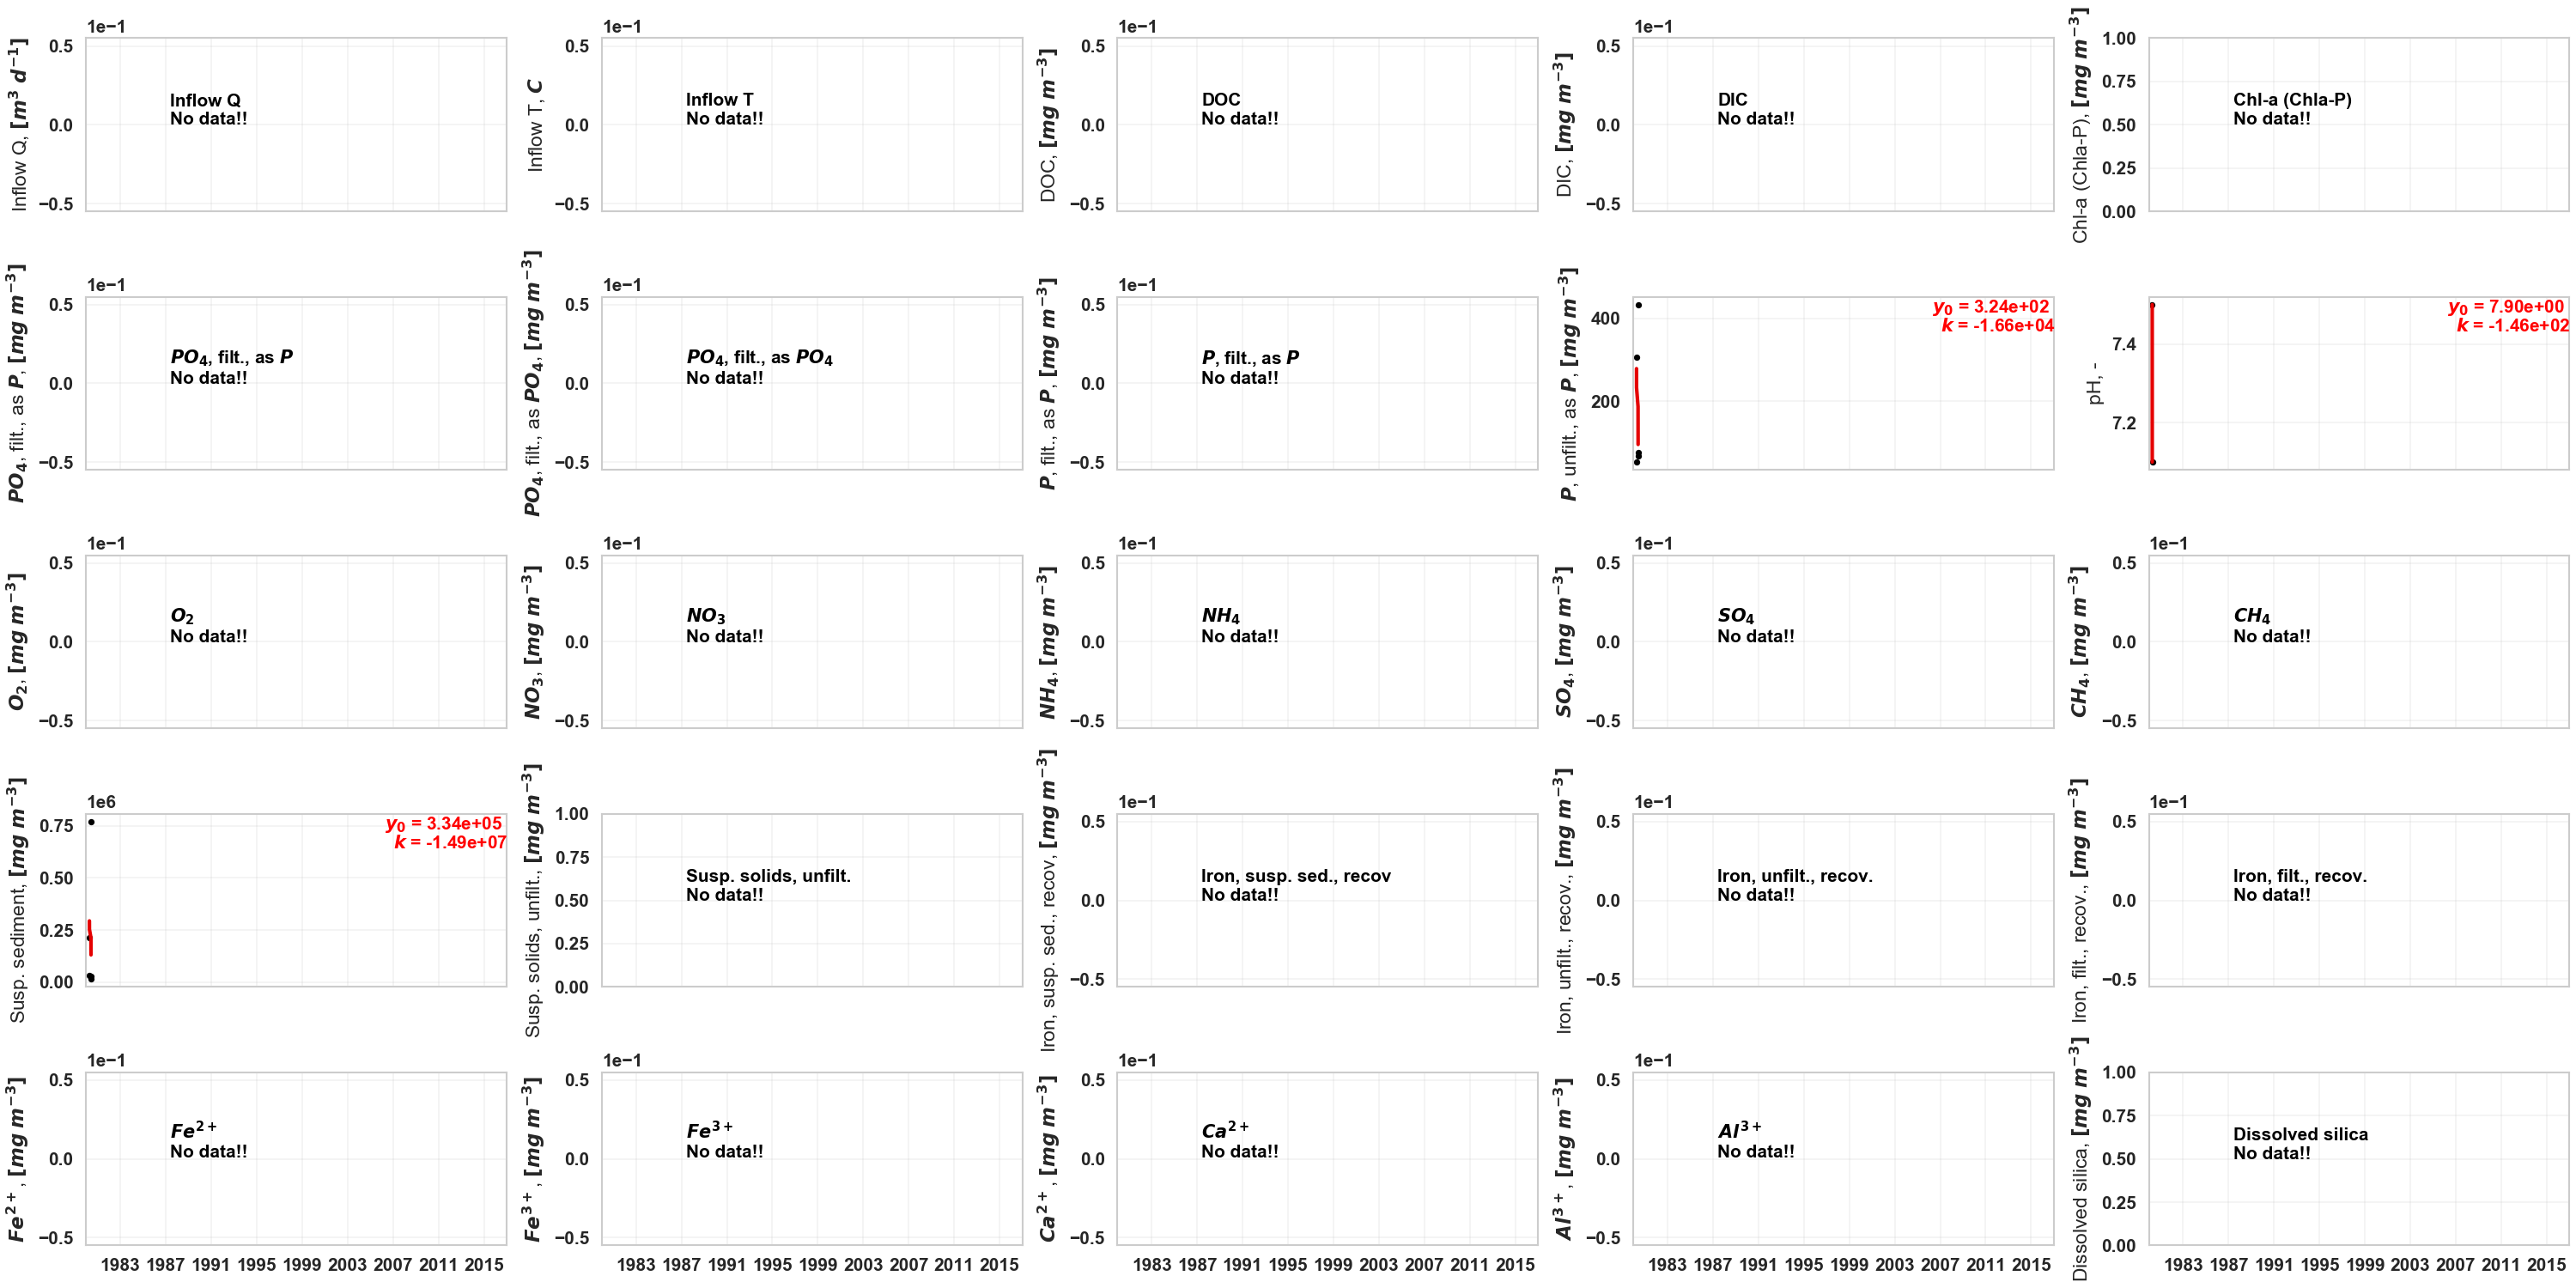
\includegraphics[width=\textwidth]{rivers/Central basin/ashtabulariver.png}
% \caption{lion!!}
\end{figure}

\end{frame}

\begin{frame}
\frametitle{Central Basin: Black river}

\begin{figure}
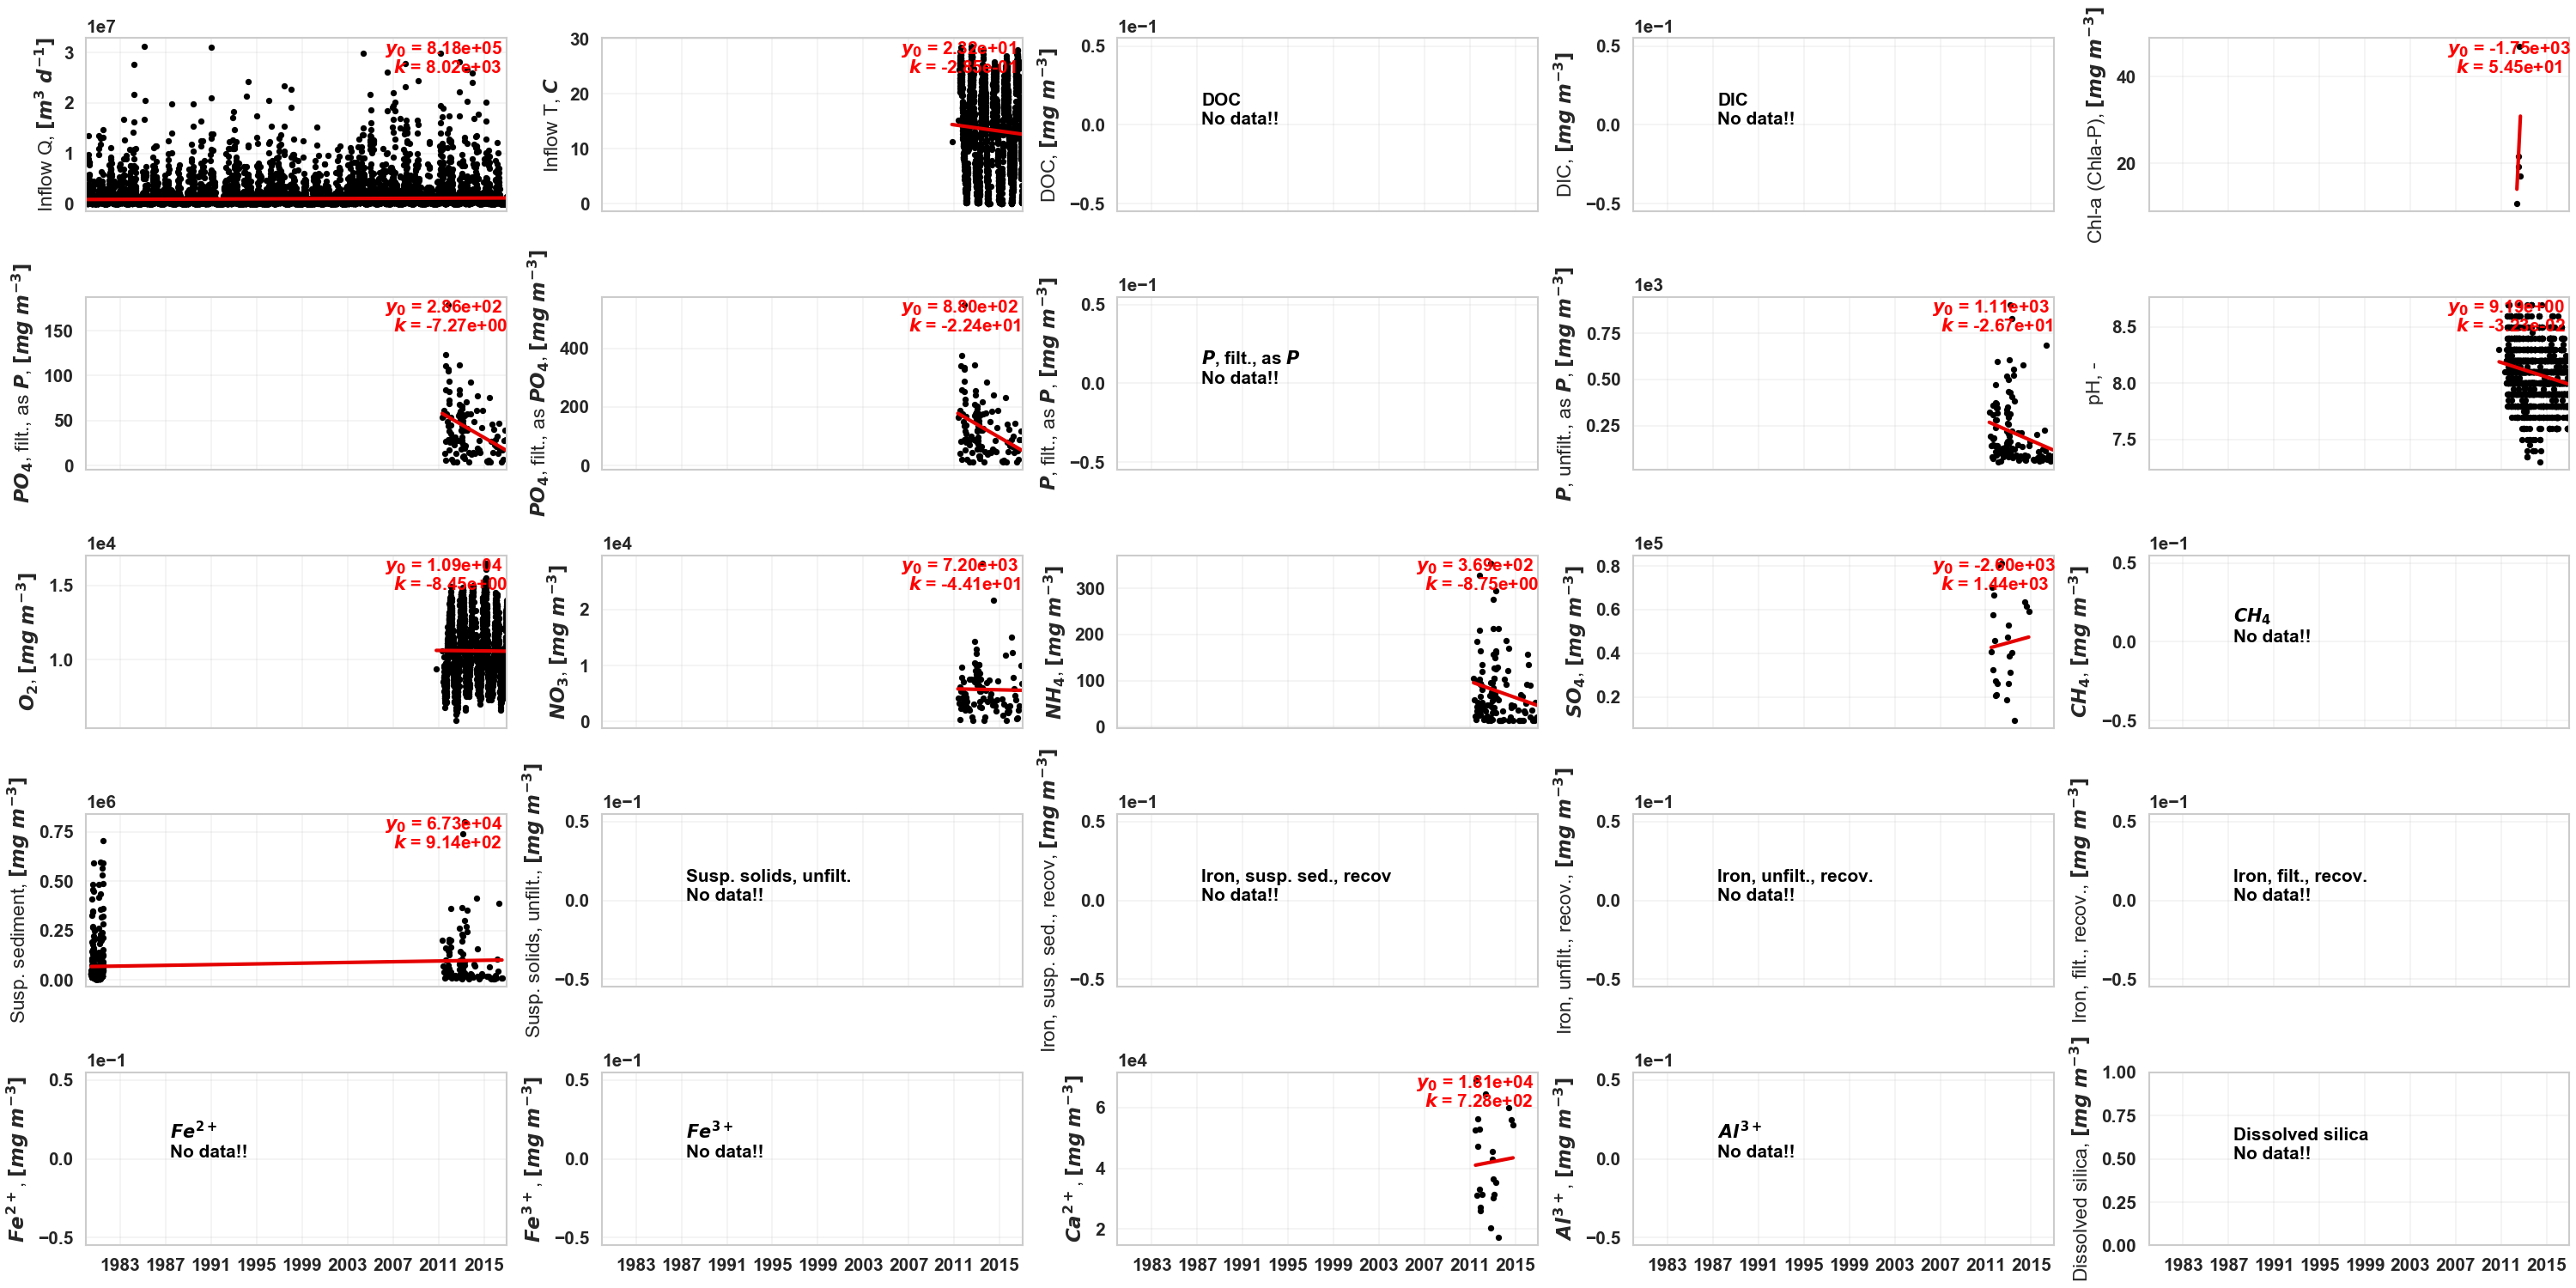
\includegraphics[width=\textwidth]{rivers/Central basin/blackriver.png}
% \caption{lion!!}
\end{figure}

\end{frame}

\begin{frame}
\frametitle{Central Basin: Chagrin river}

\begin{figure}
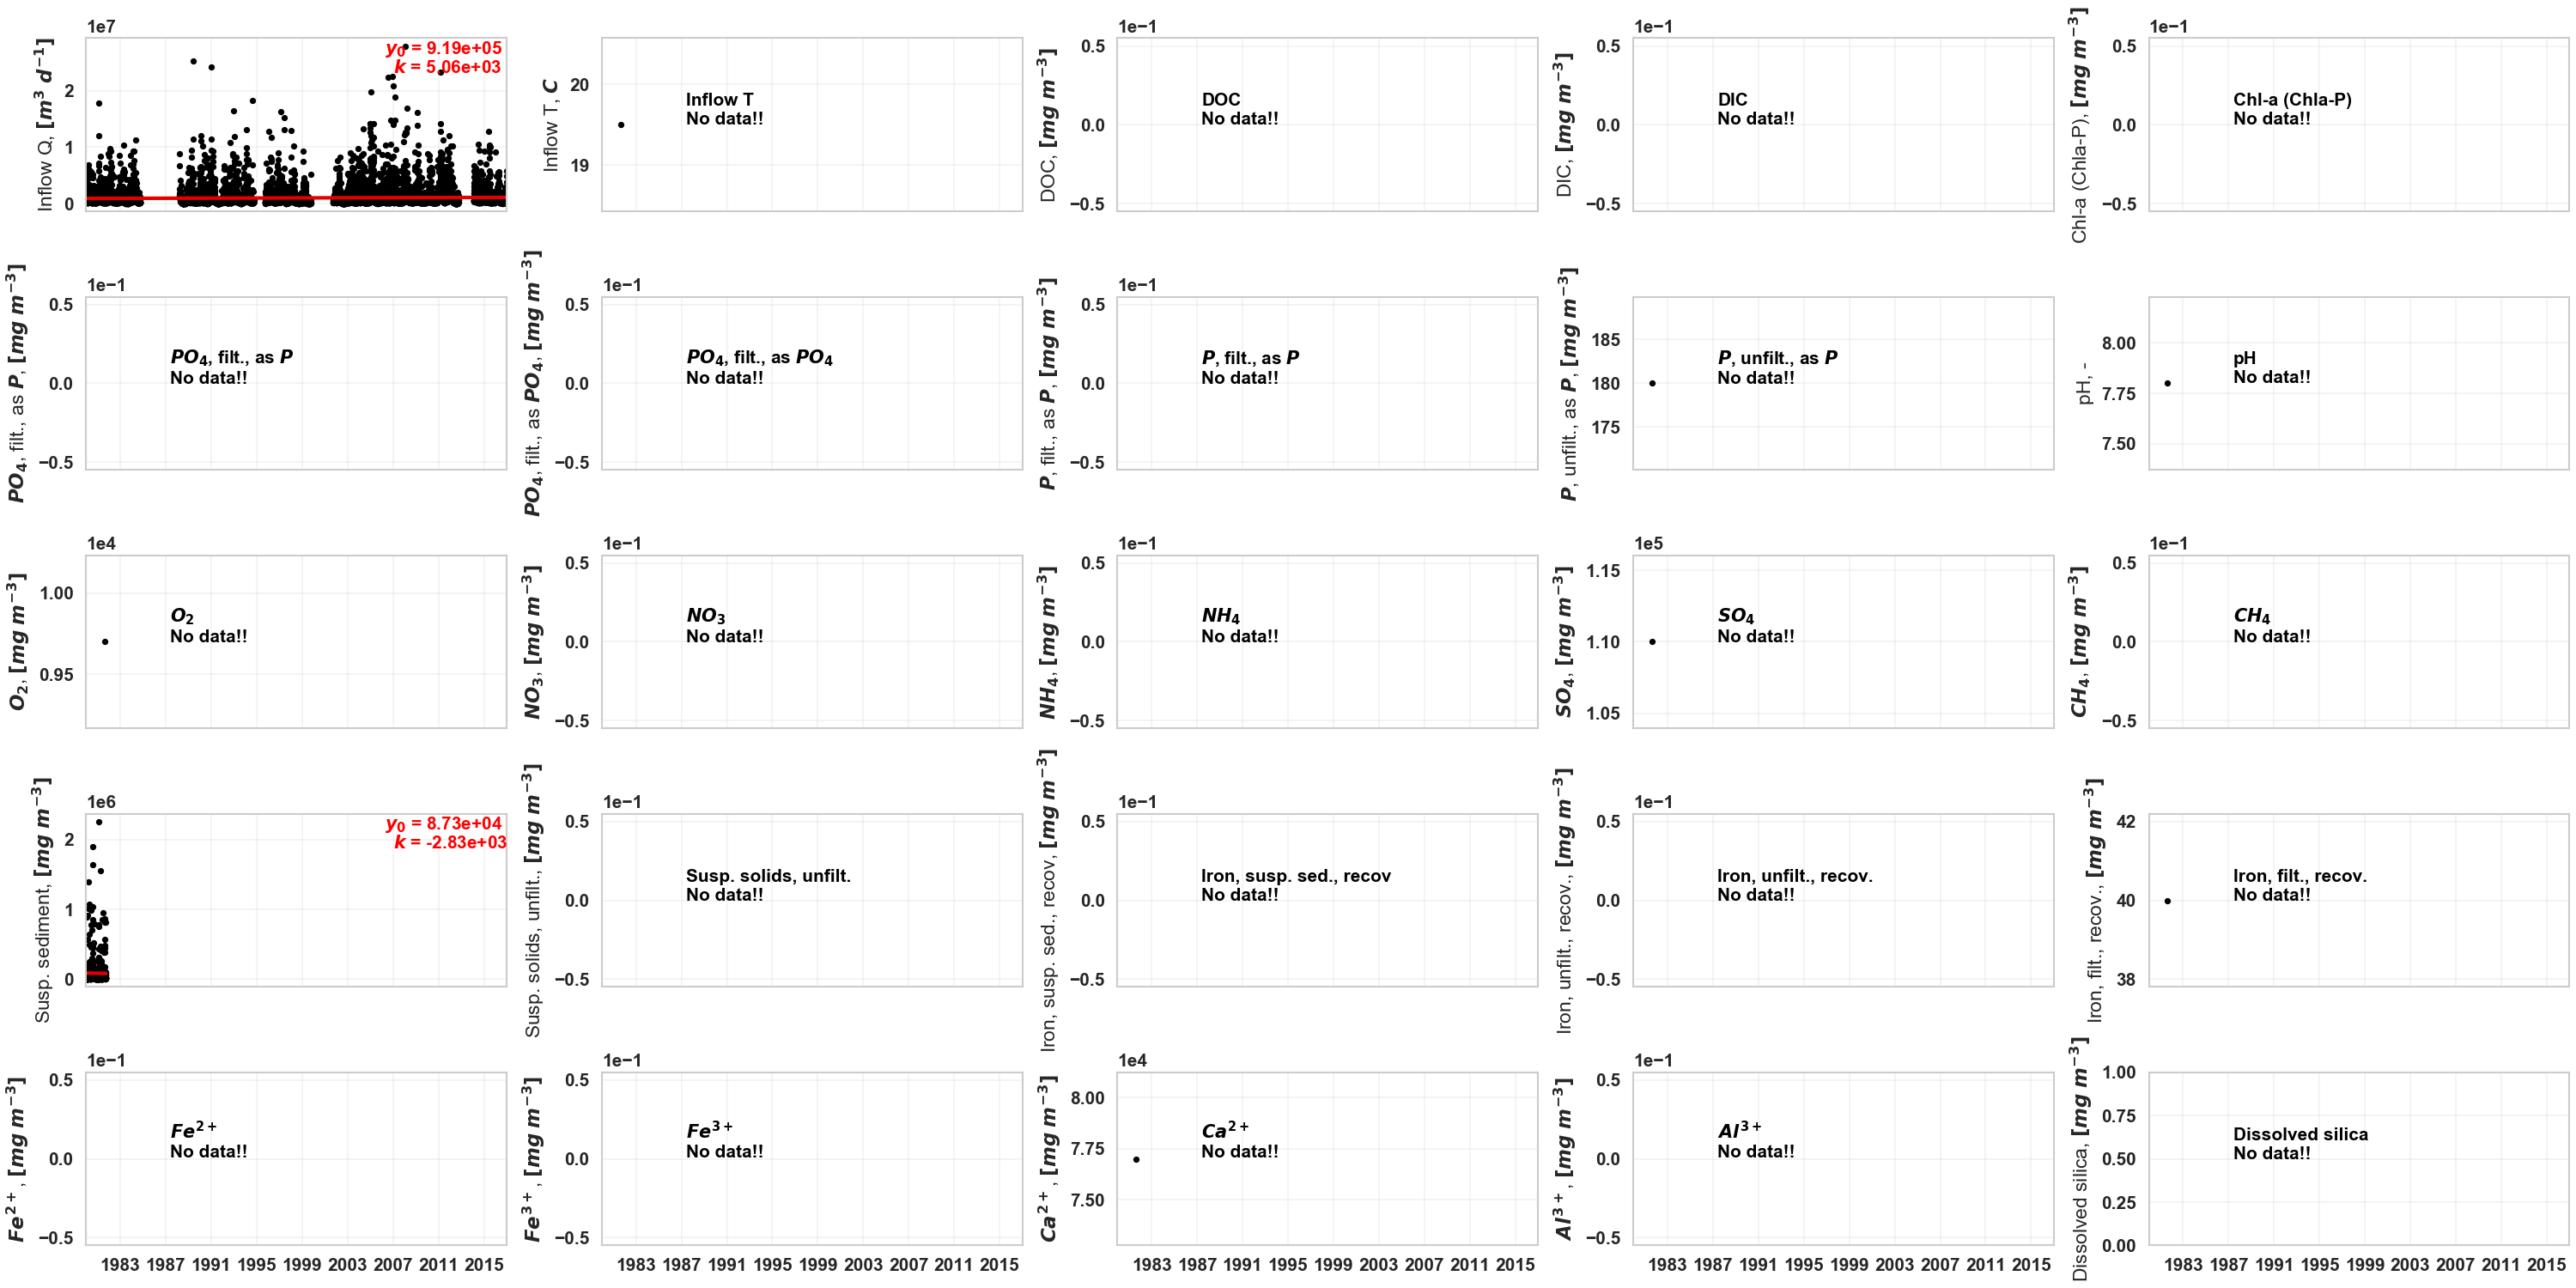
\includegraphics[width=\textwidth]{rivers/Central basin/chagrinriver.png}
% \caption{lion!!}
\end{figure}

\end{frame}

\begin{frame}
\frametitle{Central Basin: Conneaut creek}

\begin{figure}
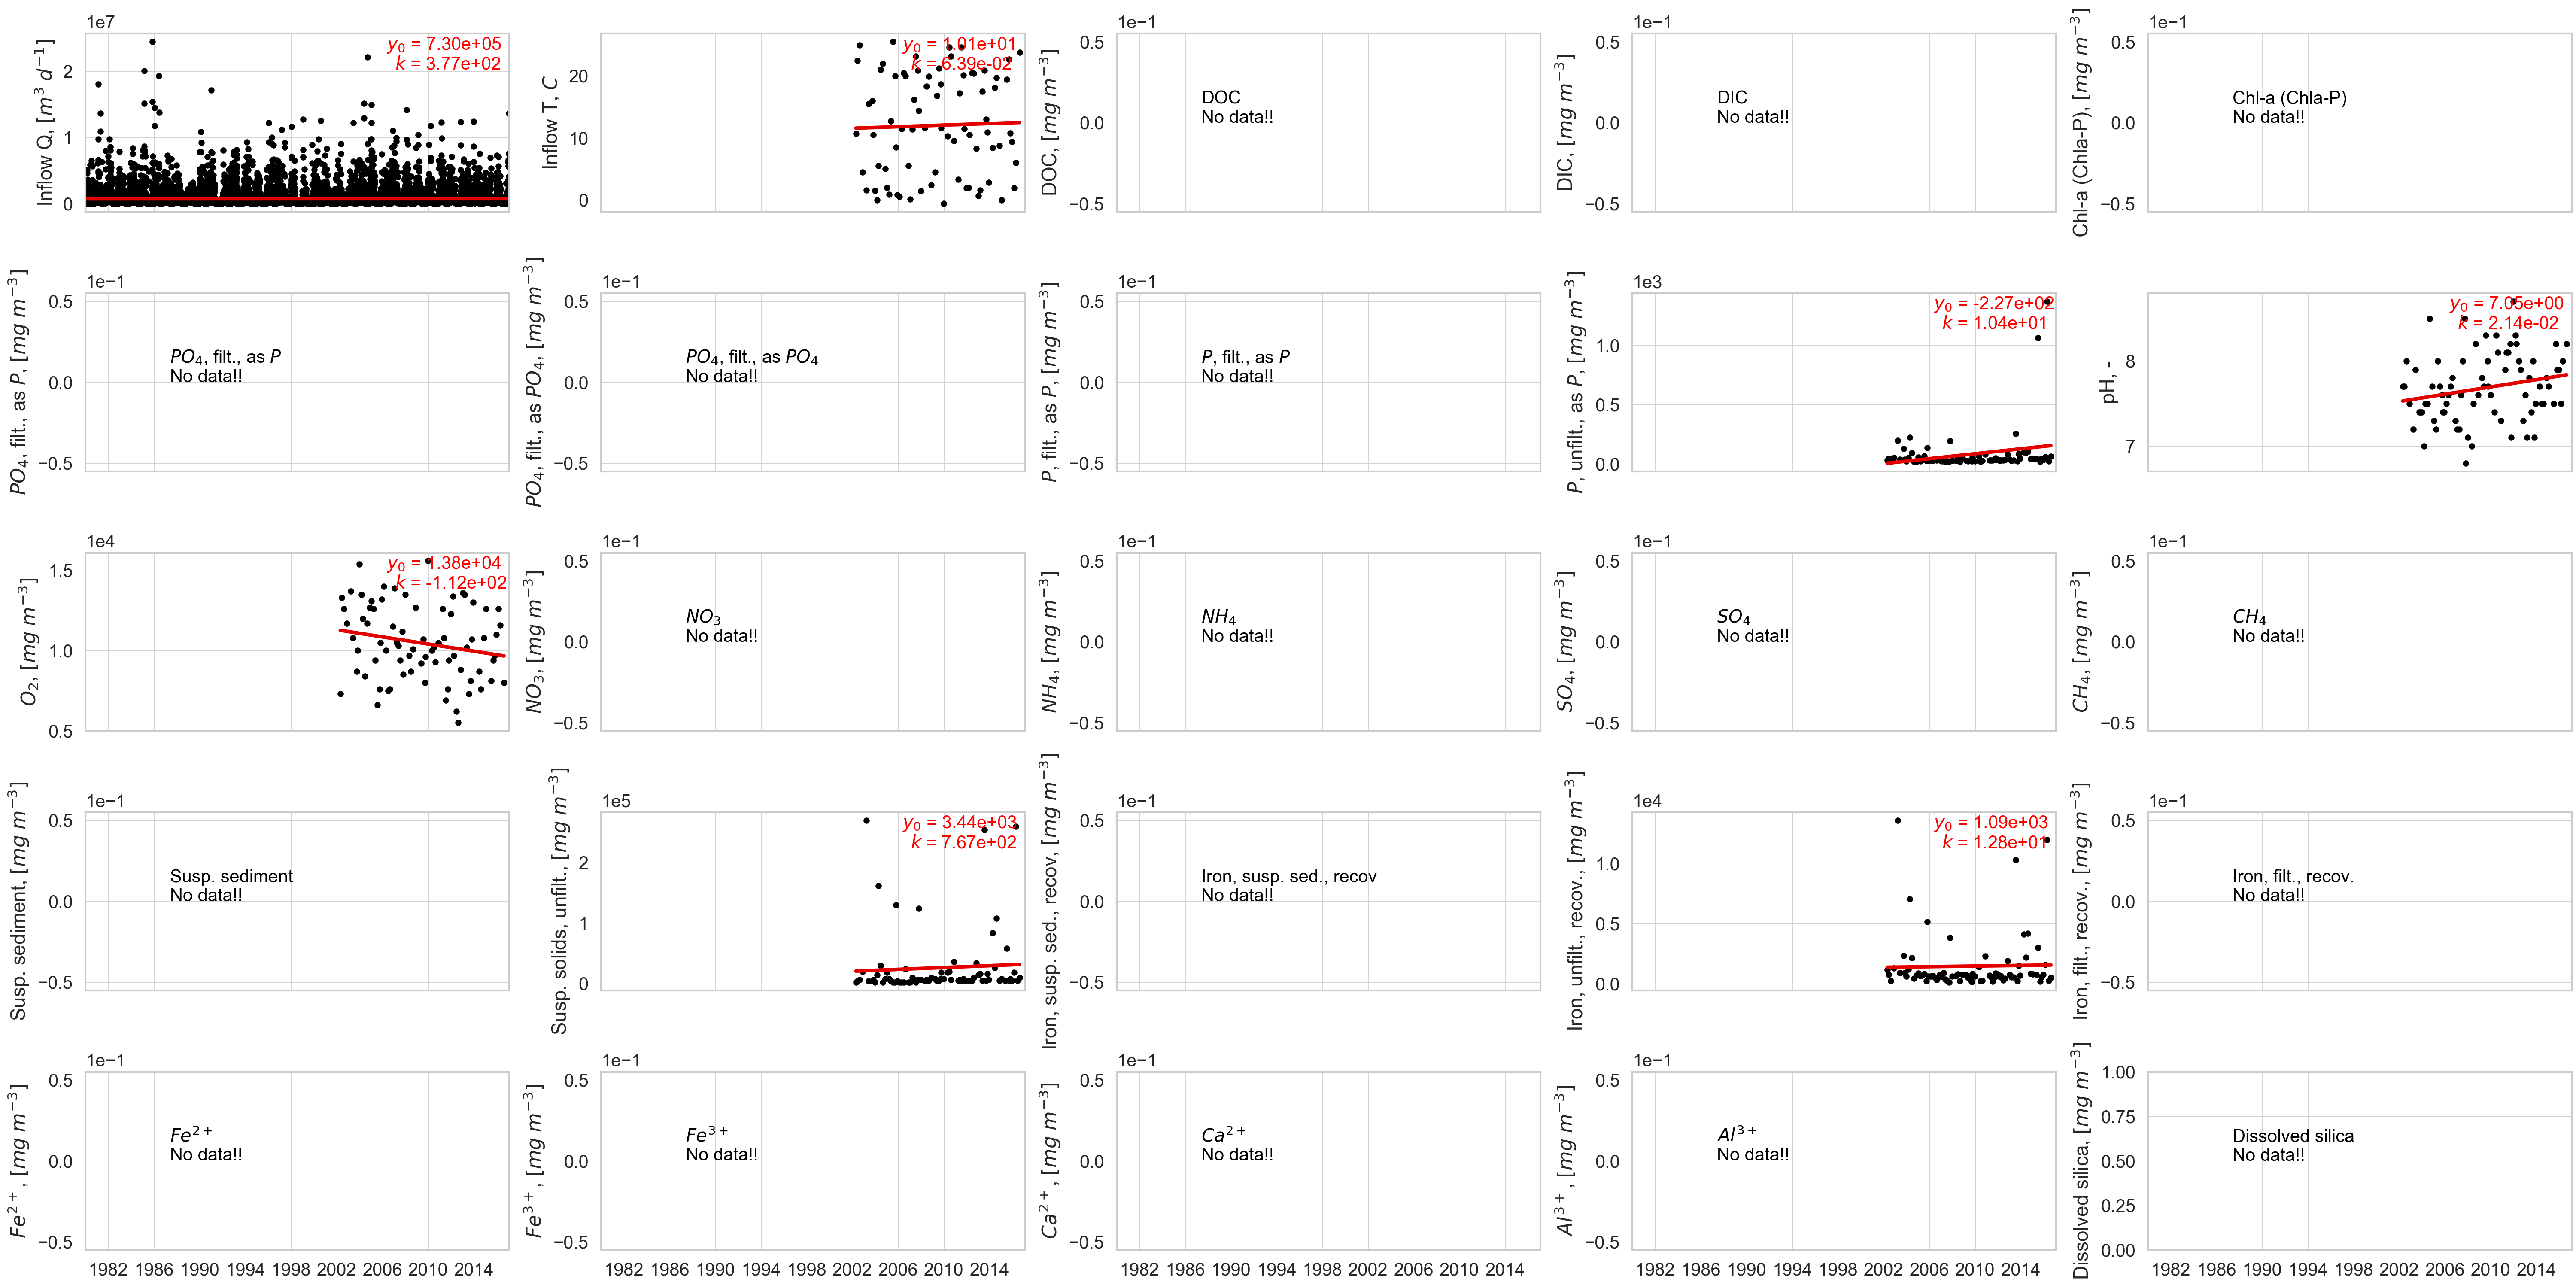
\includegraphics[width=\textwidth]{rivers/Central basin/conneautcreek.png}
% \caption{lion!!}
\end{figure}

\end{frame}

\begin{frame}
\frametitle{Central Basin: Cuyahoga river}

\begin{figure}
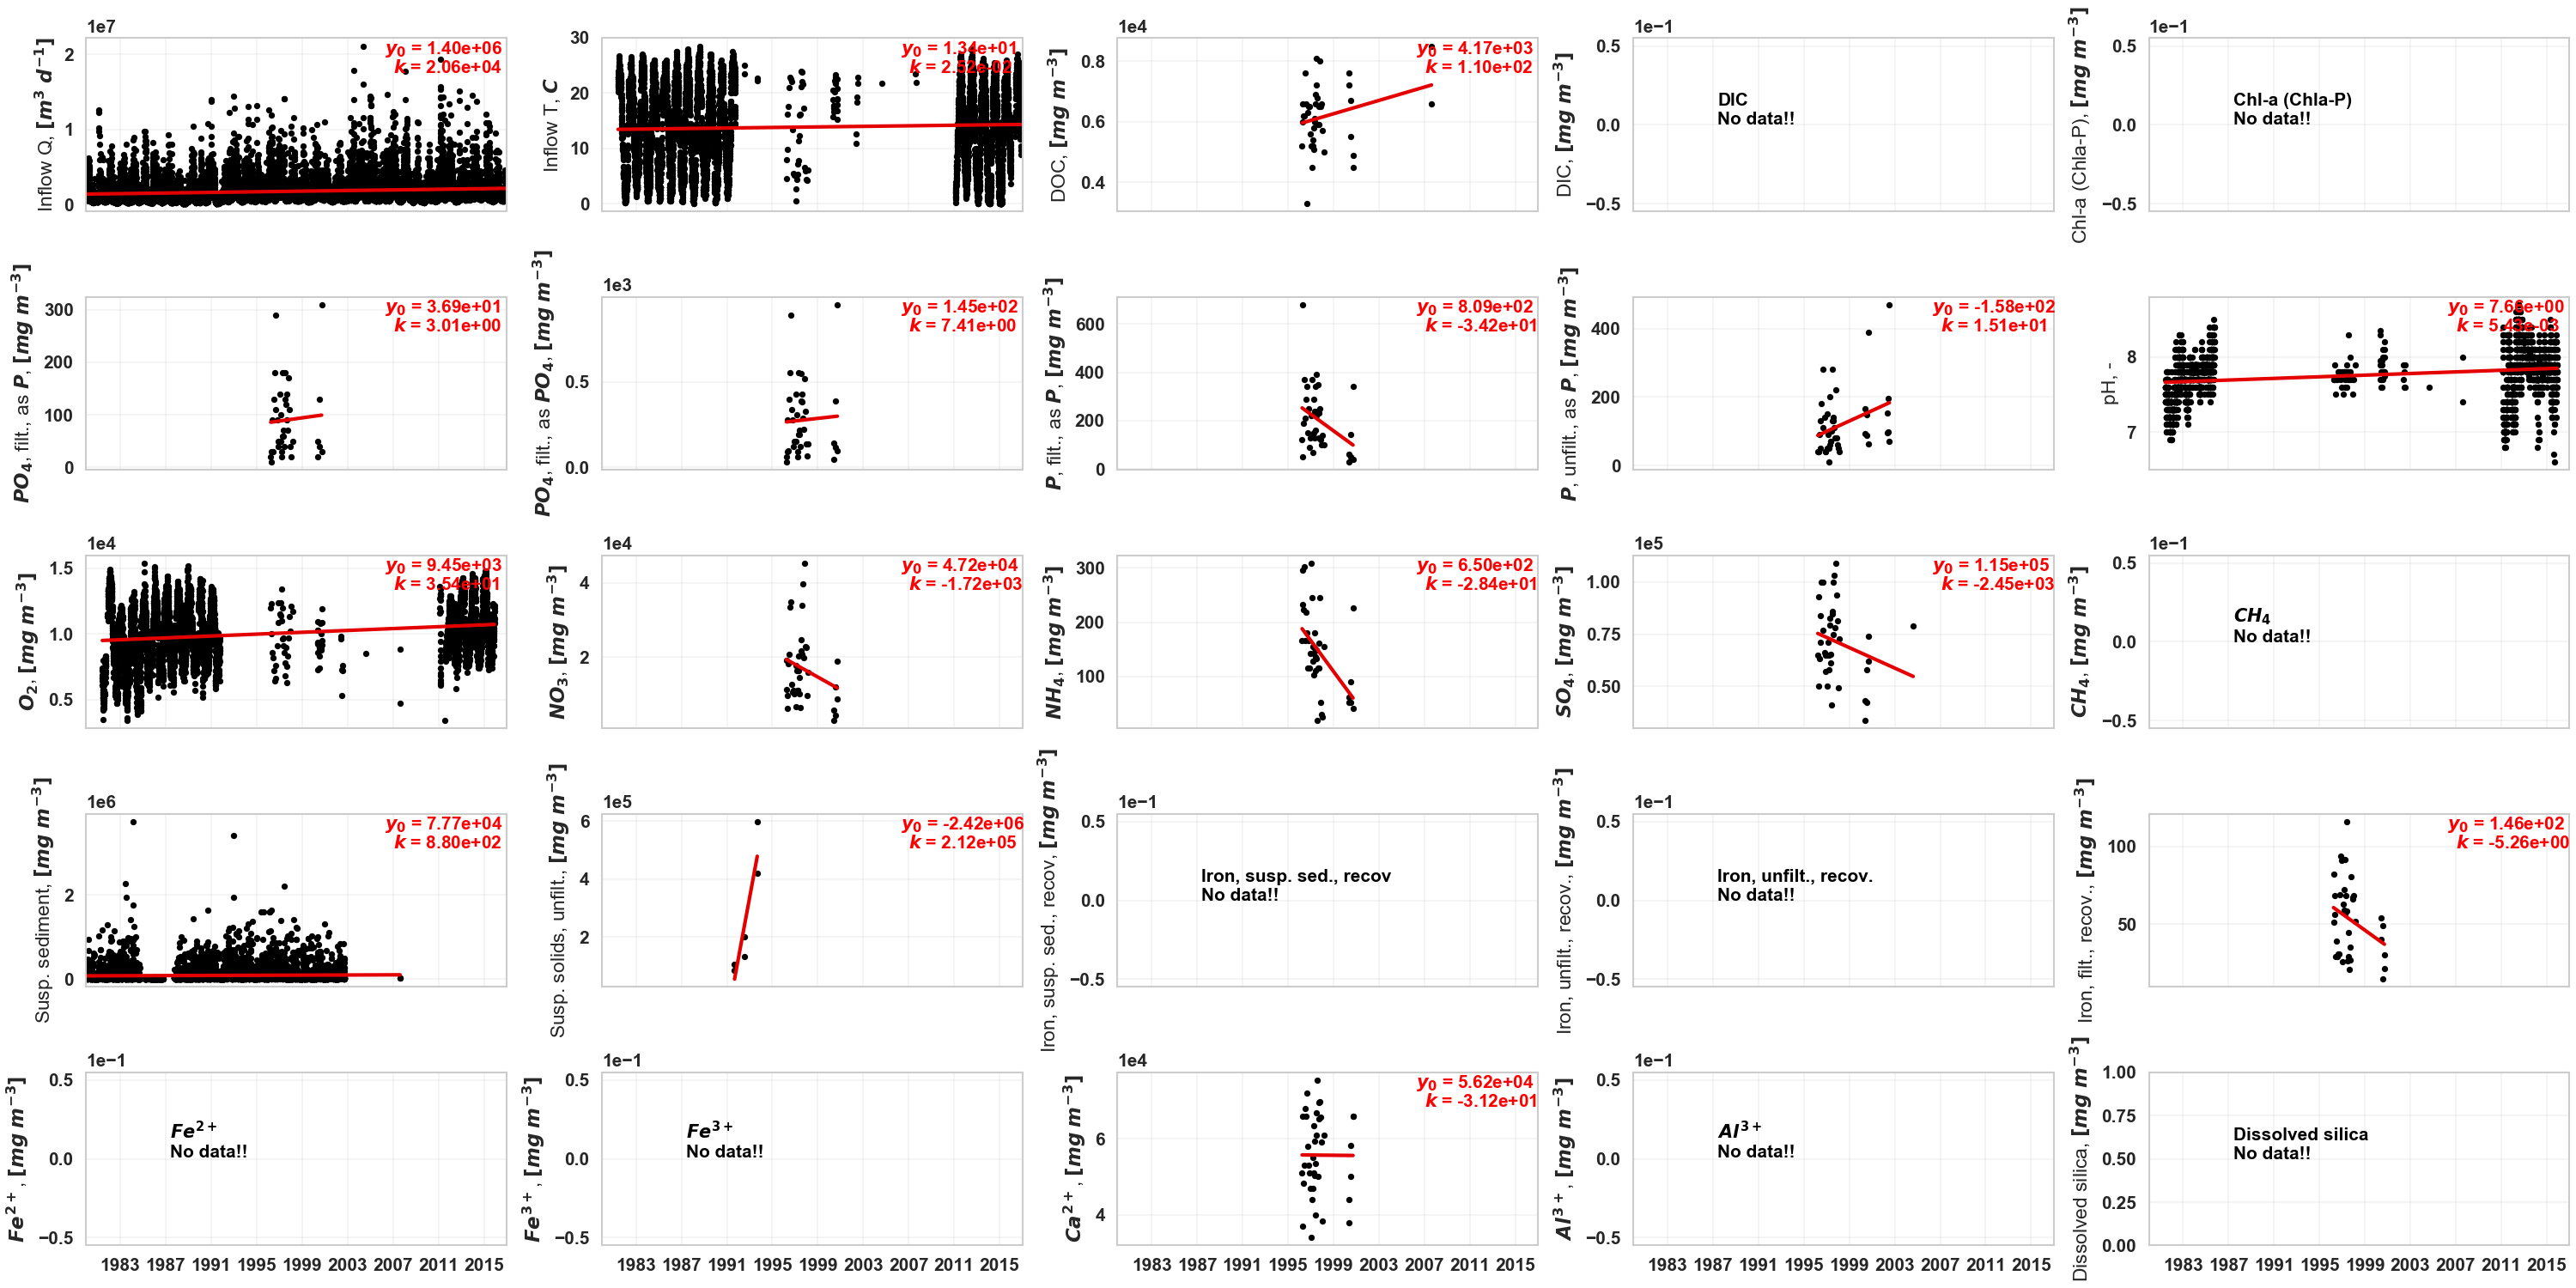
\includegraphics[width=\textwidth]{rivers/Central basin/cuyahogariver.png}
% \caption{lion!!}
\end{figure}

\end{frame}

\begin{frame}
\frametitle{Central Basin: Grand river}

\begin{figure}
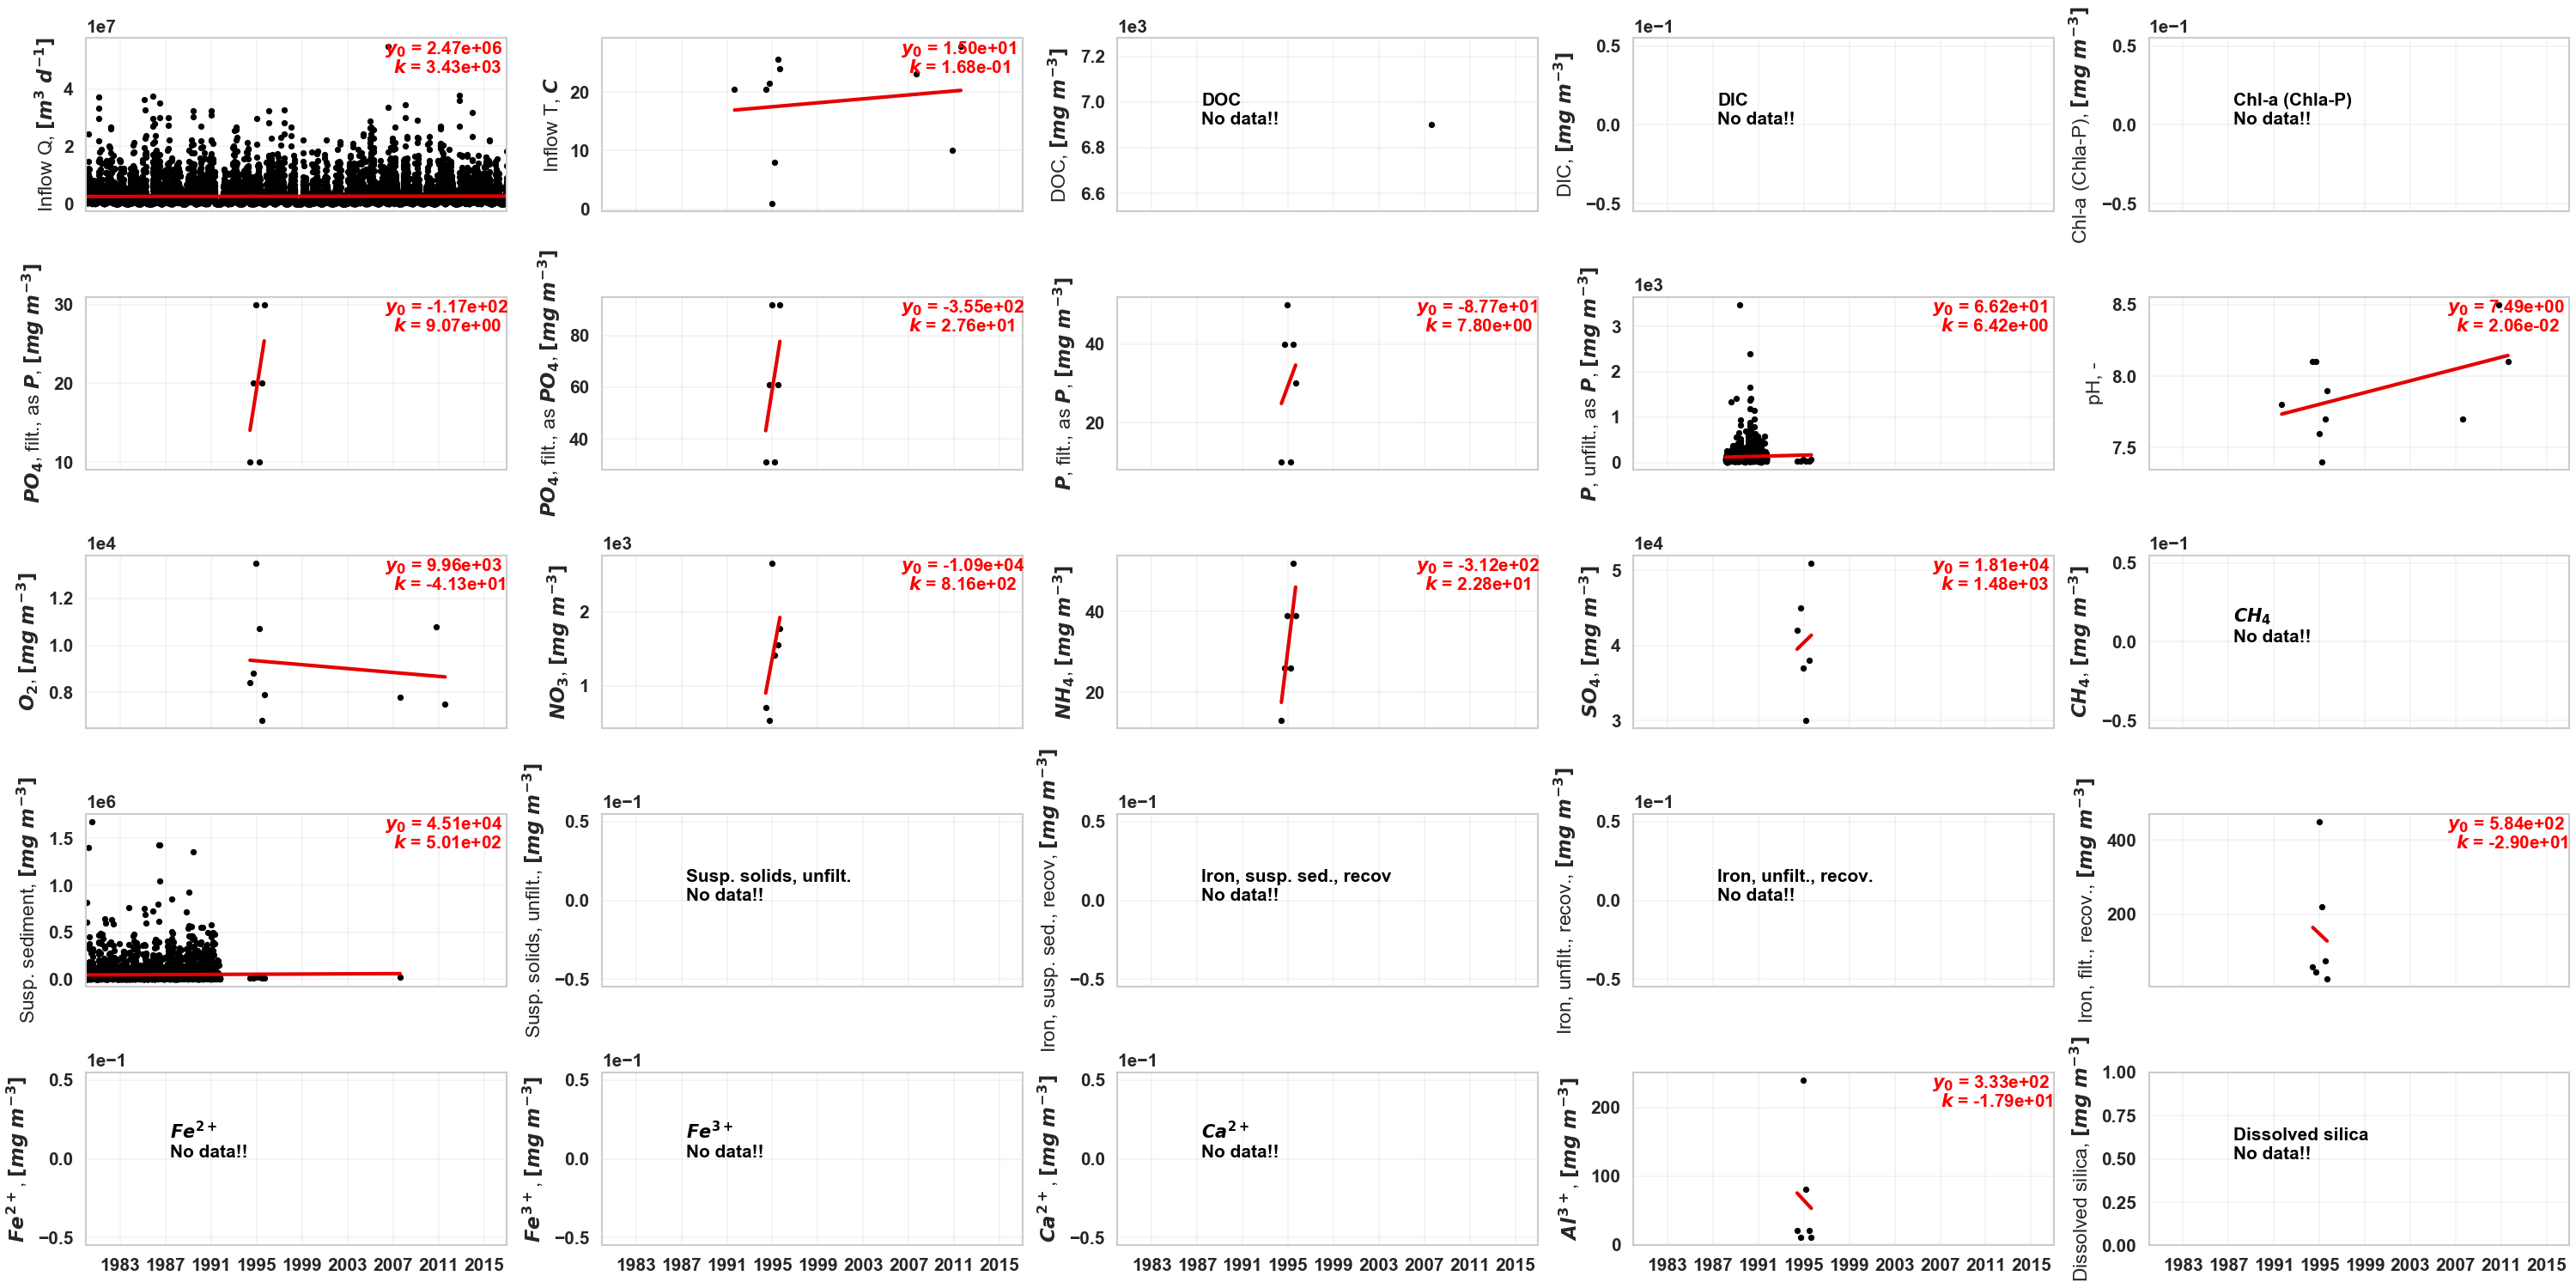
\includegraphics[width=\textwidth]{rivers/Central basin/grandriver.png}
% \caption{lion!!}
\end{figure}

\end{frame}

\begin{frame}
\frametitle{Central Basin: Rocky river}

\begin{figure}
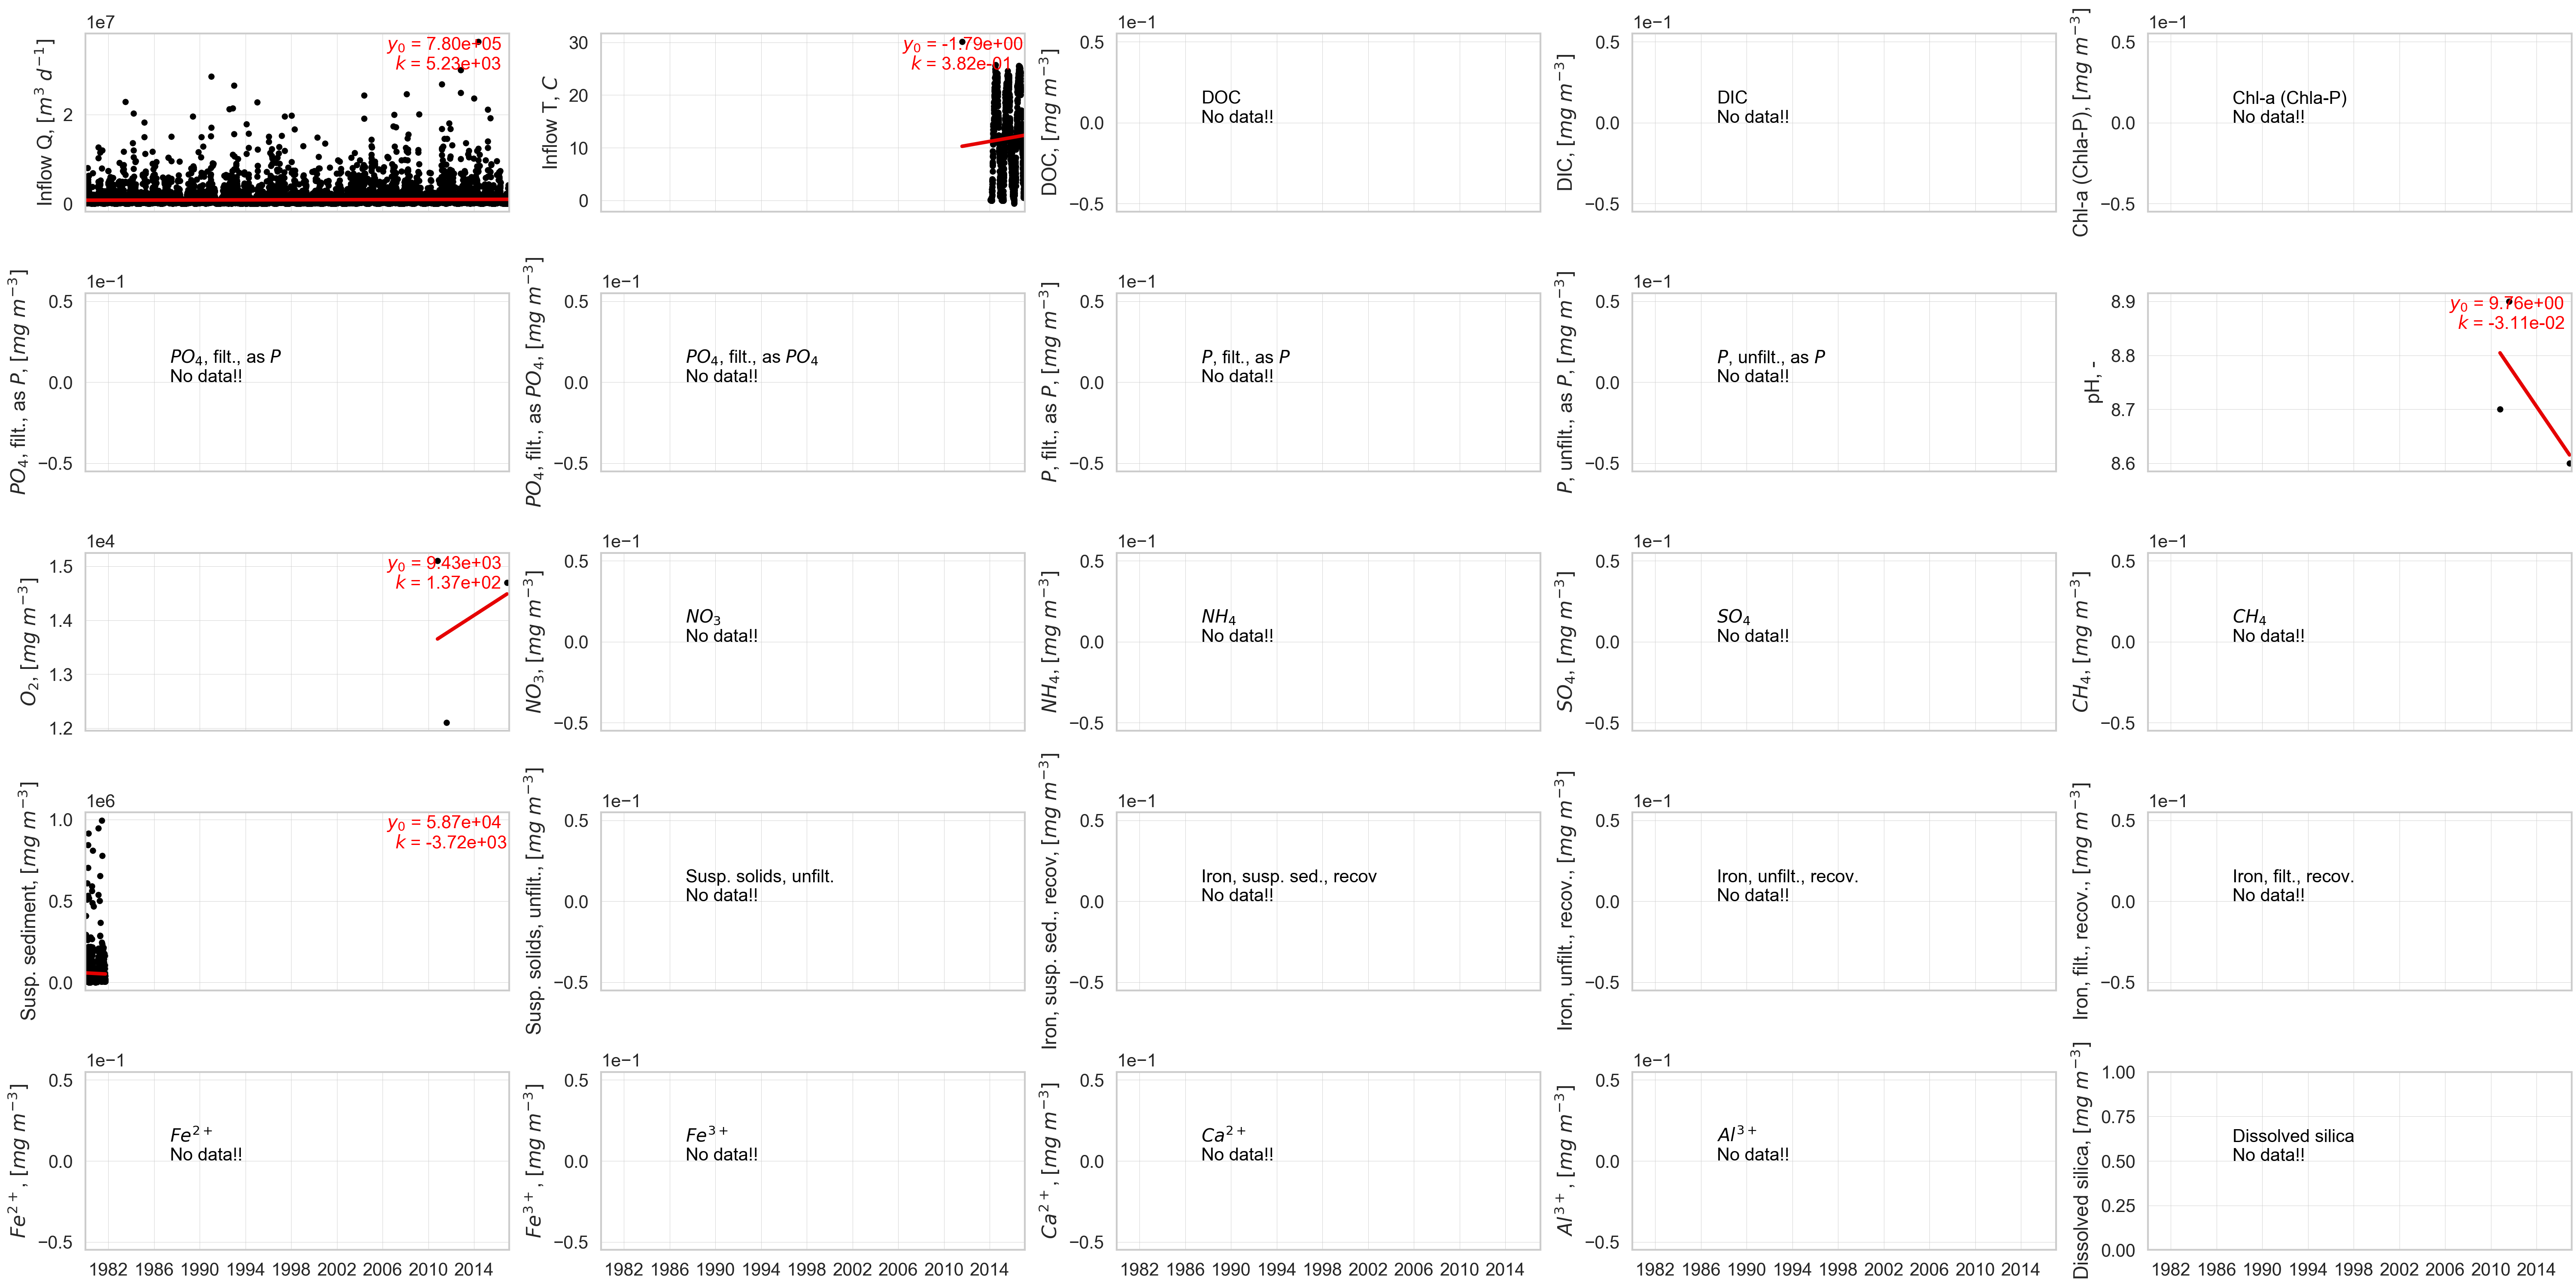
\includegraphics[width=\textwidth]{rivers/Central basin/rockyriver.png}
% \caption{lion!!}
\end{figure}

\end{frame}

\begin{frame}
\frametitle{Central Basin: Sandusky river}

\begin{figure}
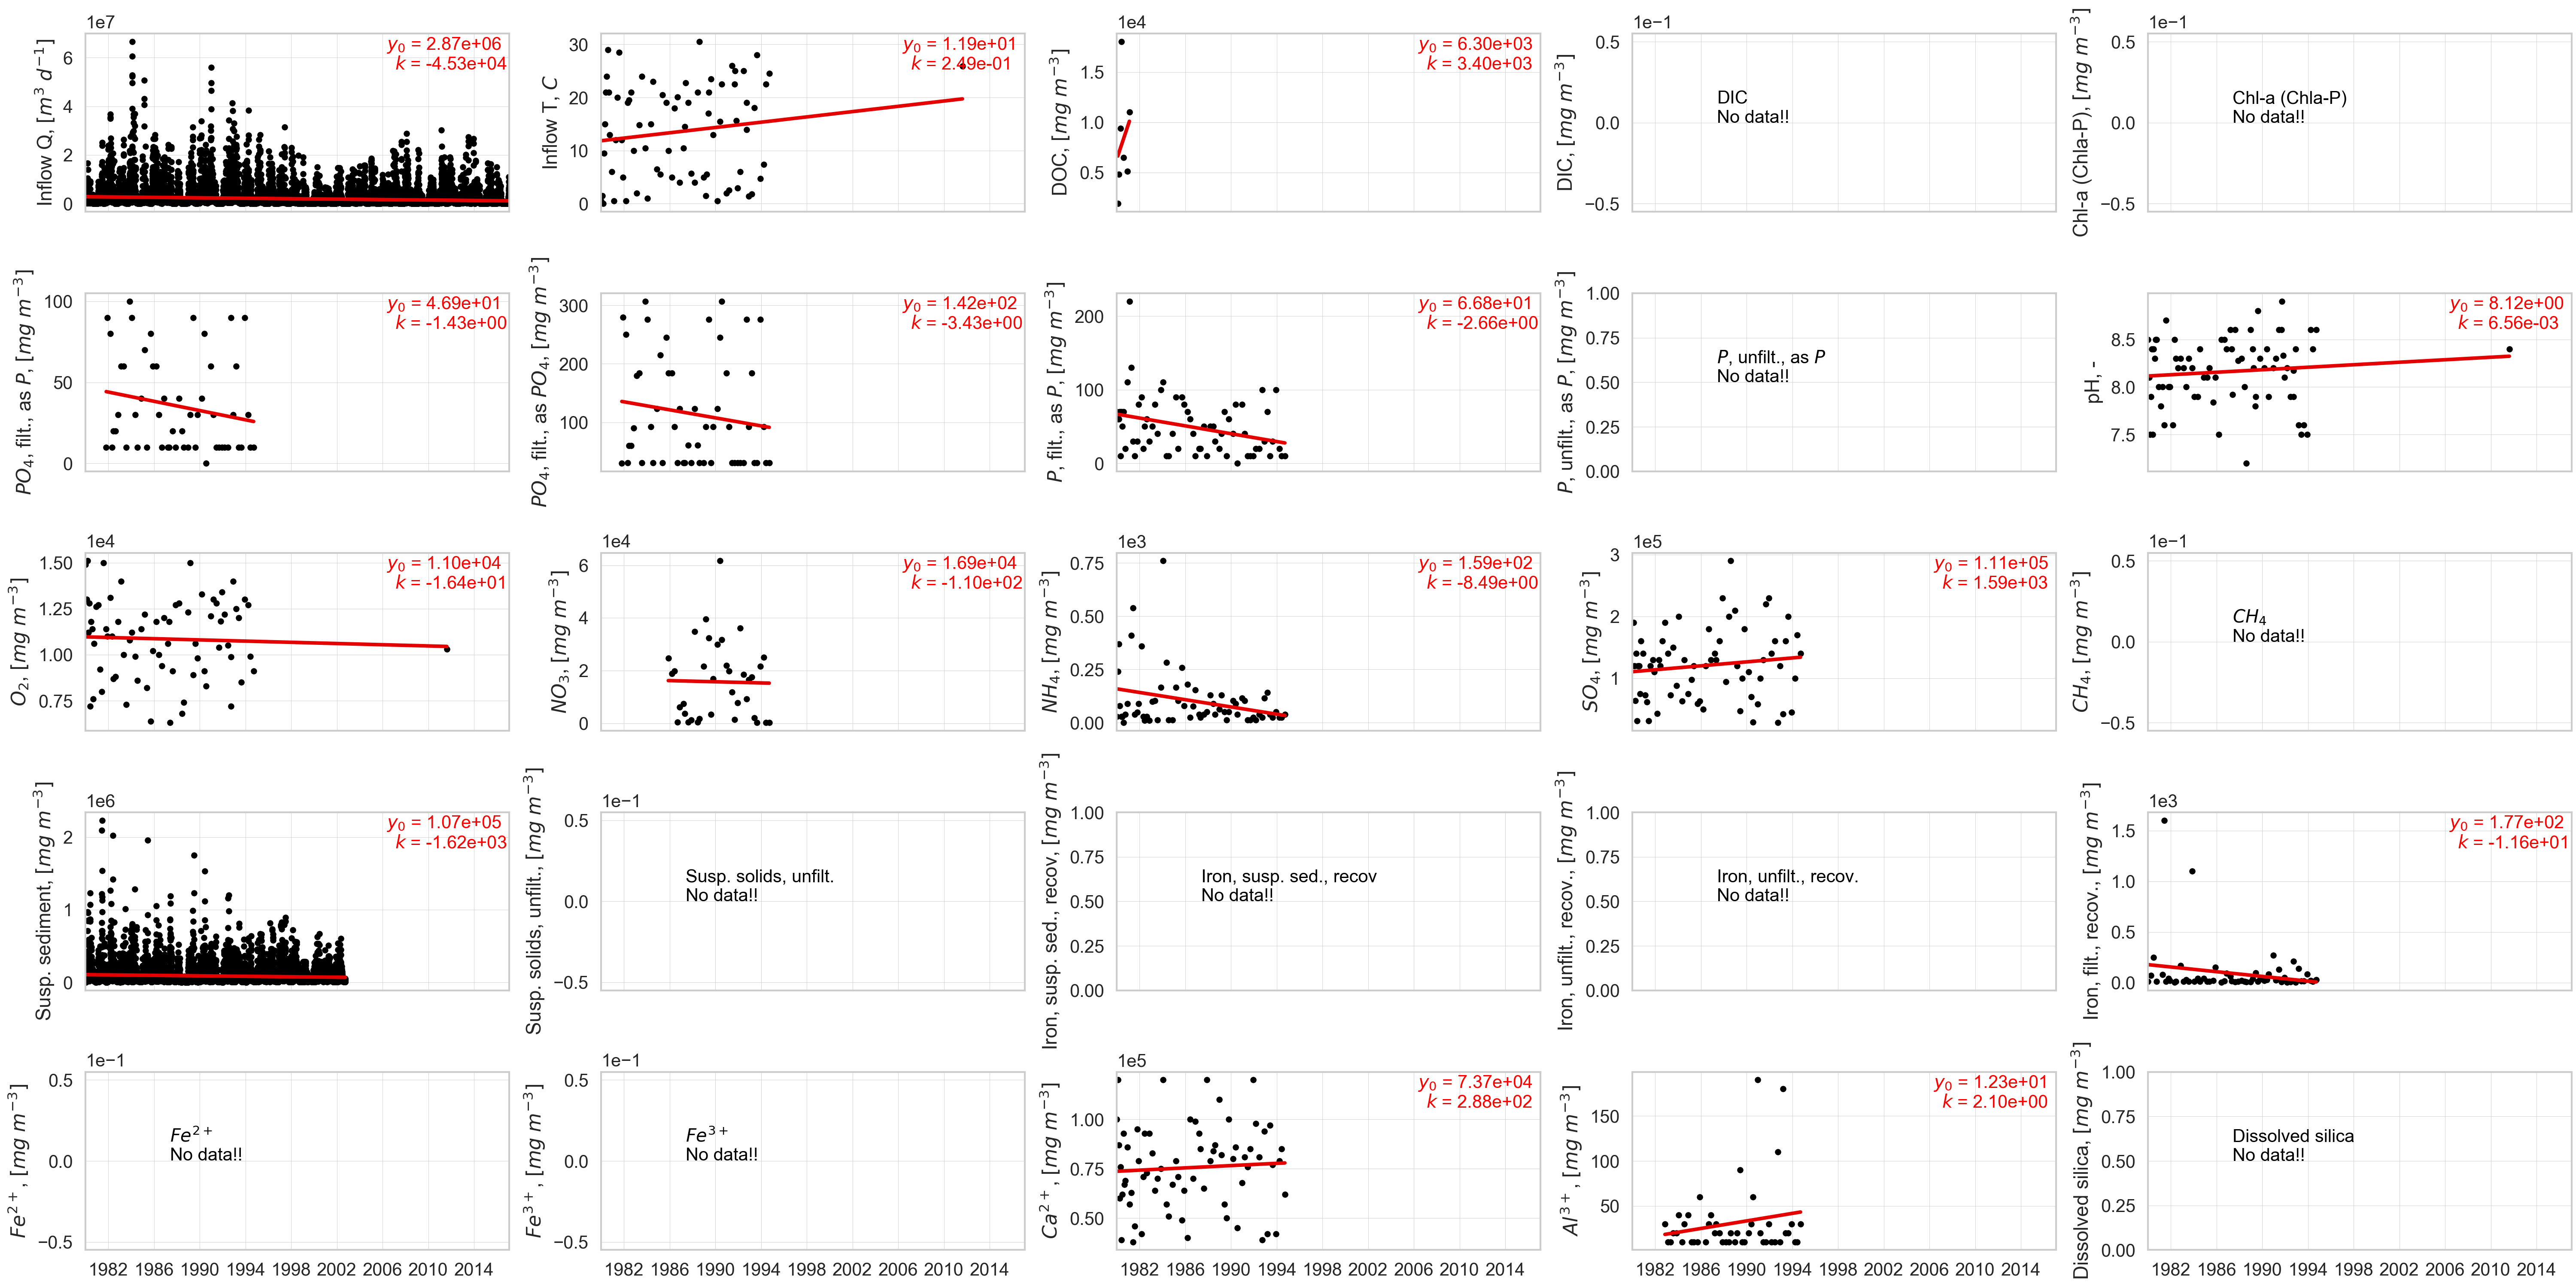
\includegraphics[width=\textwidth]{rivers/Central basin/sanduskyriver.png}
% \caption{lion!!}
\end{figure}

\end{frame}

\begin{frame}
\frametitle{Central Basin: South-western Huron river}

\begin{figure}
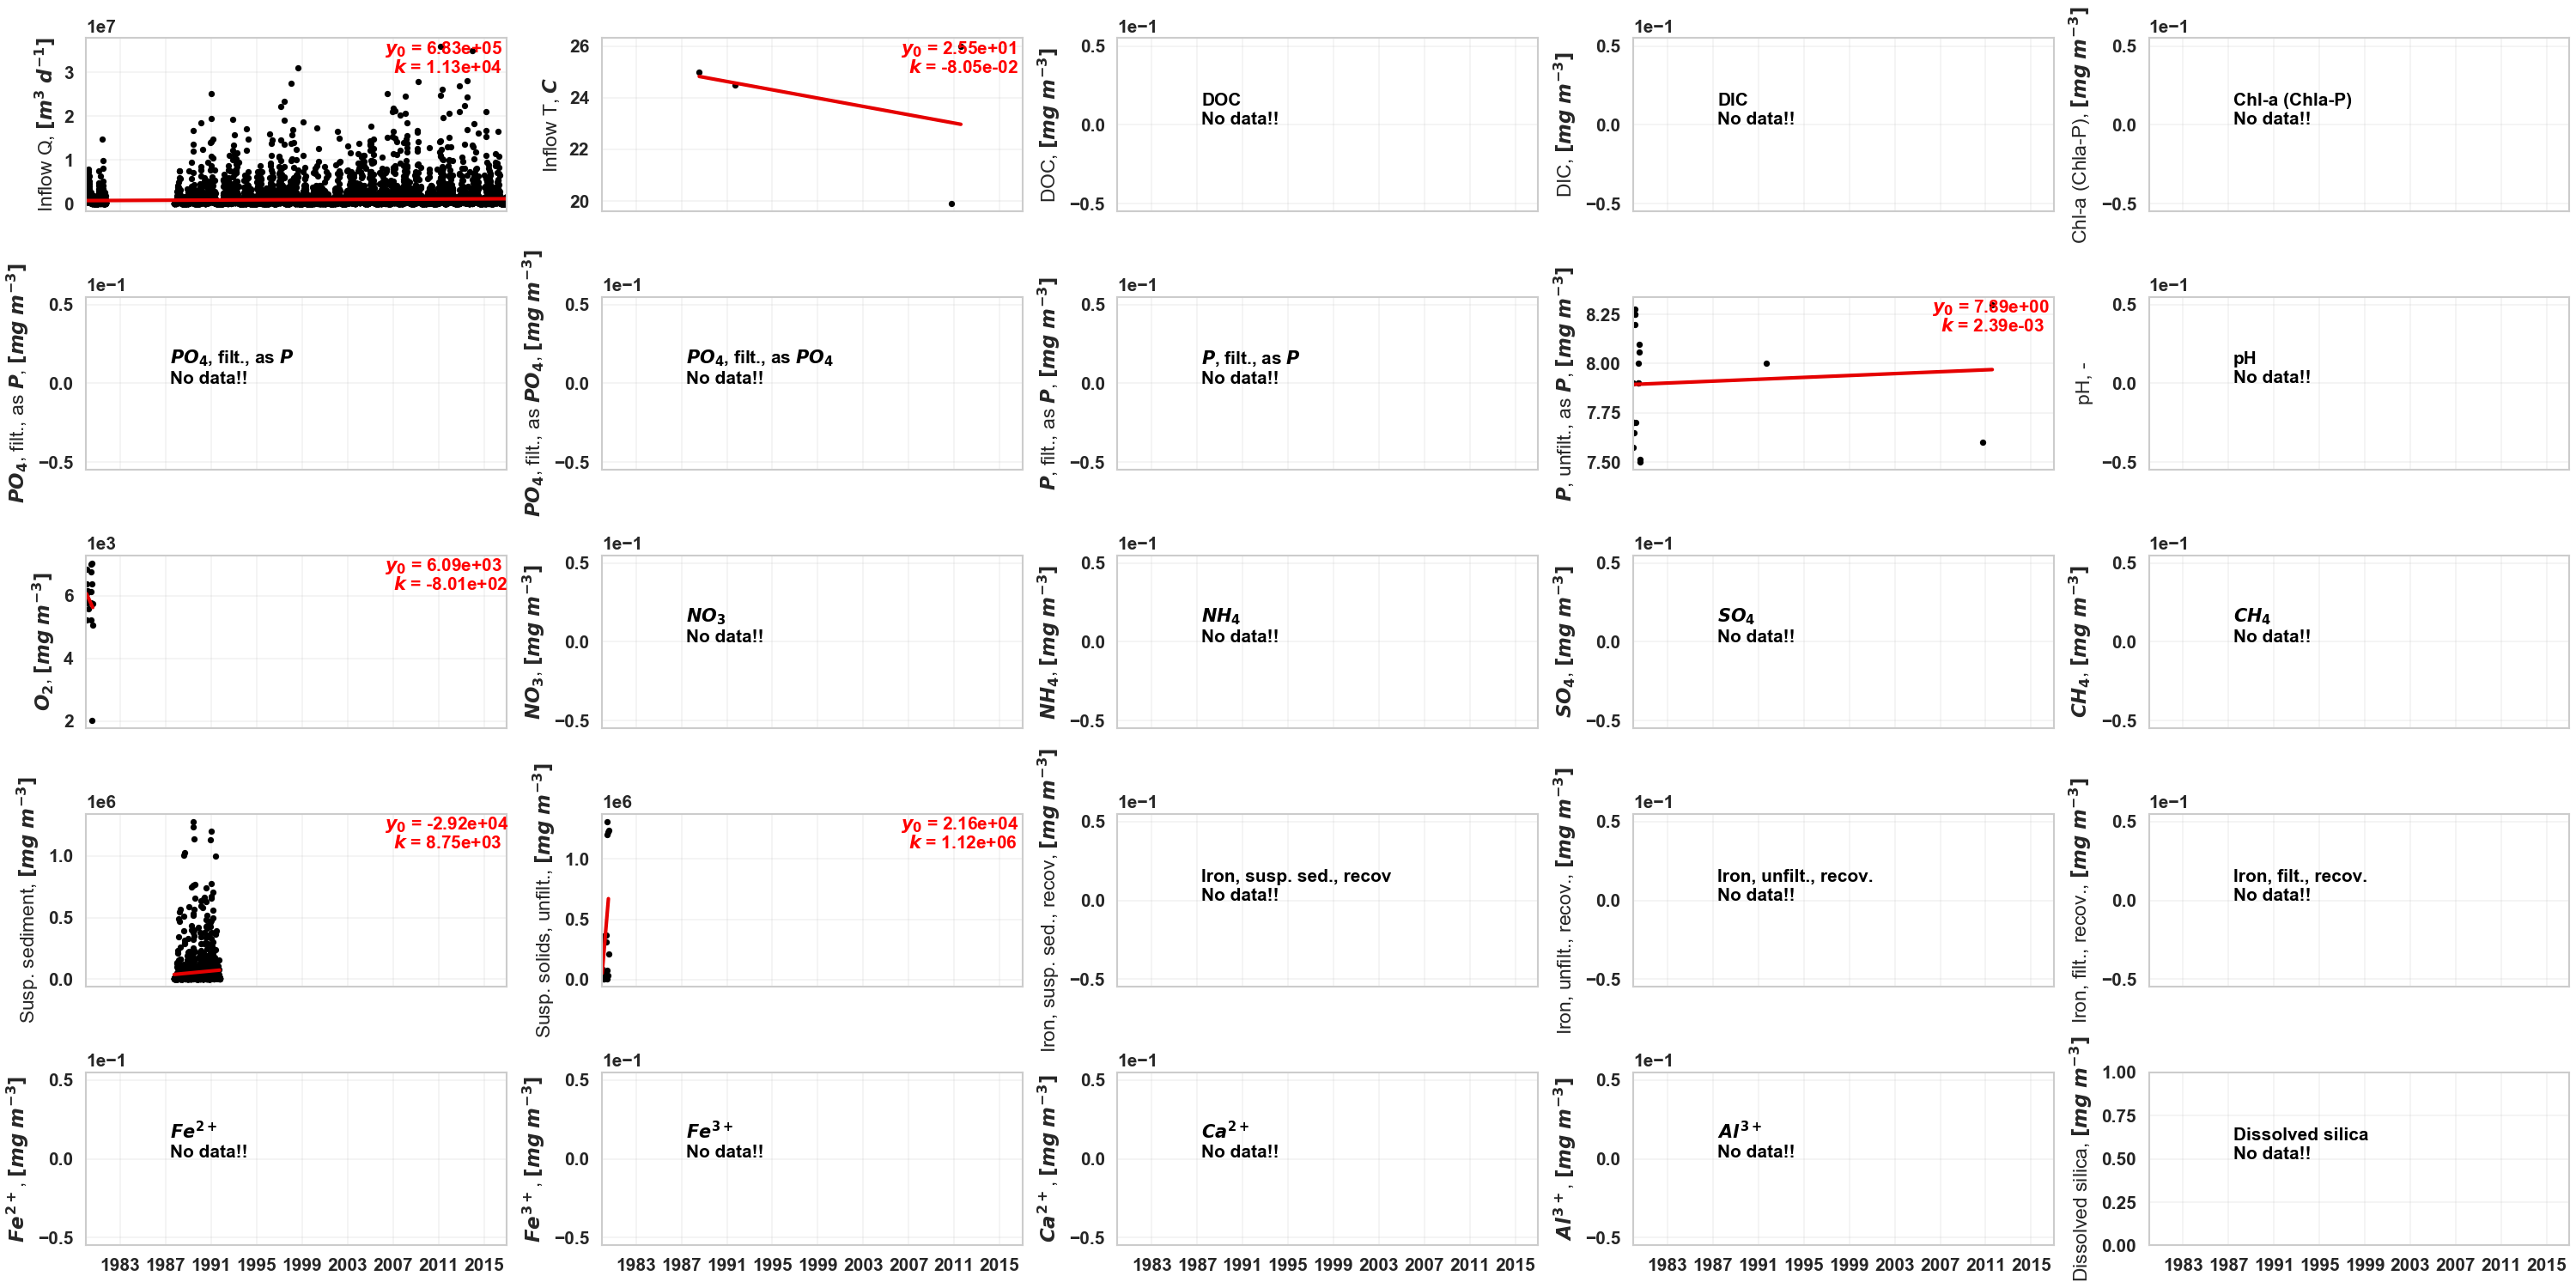
\includegraphics[width=\textwidth]{rivers/Central basin/southwesternhuronriver.png}
% \caption{lion!!}
\end{figure}

\end{frame}

\begin{frame}
\frametitle{Central Basin: Vermillion river}

\begin{figure}
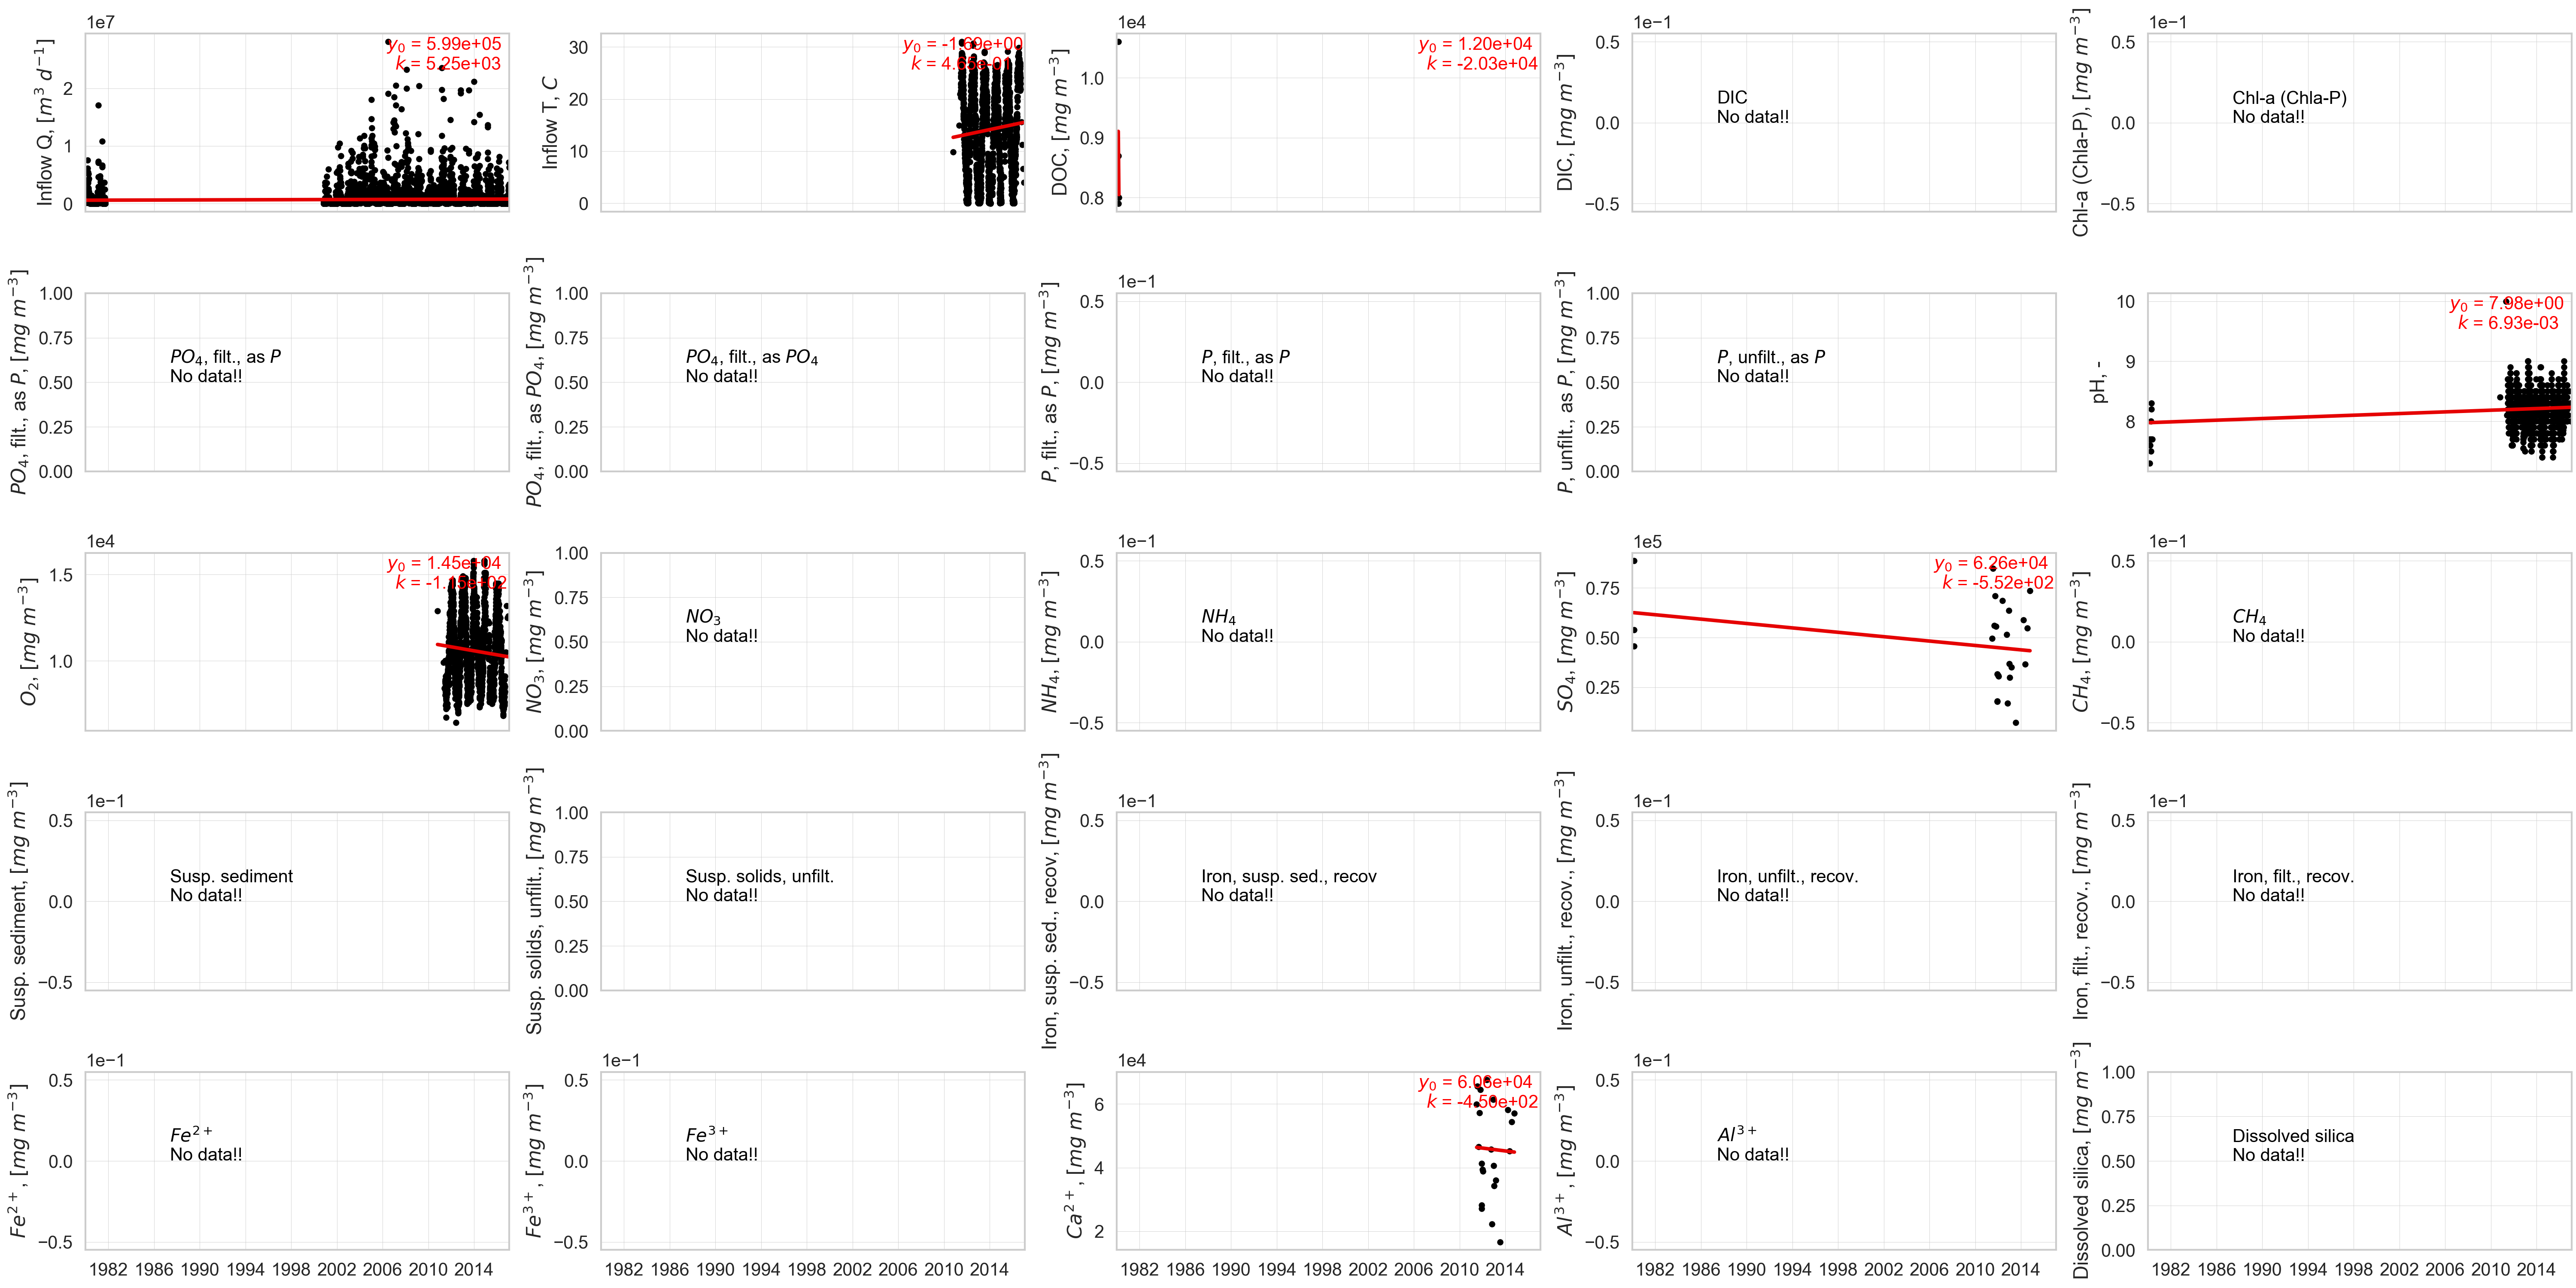
\includegraphics[width=\textwidth]{rivers/Central basin/vermillion.png}
% \caption{lion!!}
\end{figure}

\end{frame}


\subsection{Eastern Basin}
\label{sub:eastern_basin}


\begin{frame}
\frametitle{Eastern Basin: Niagara river}

\begin{figure}
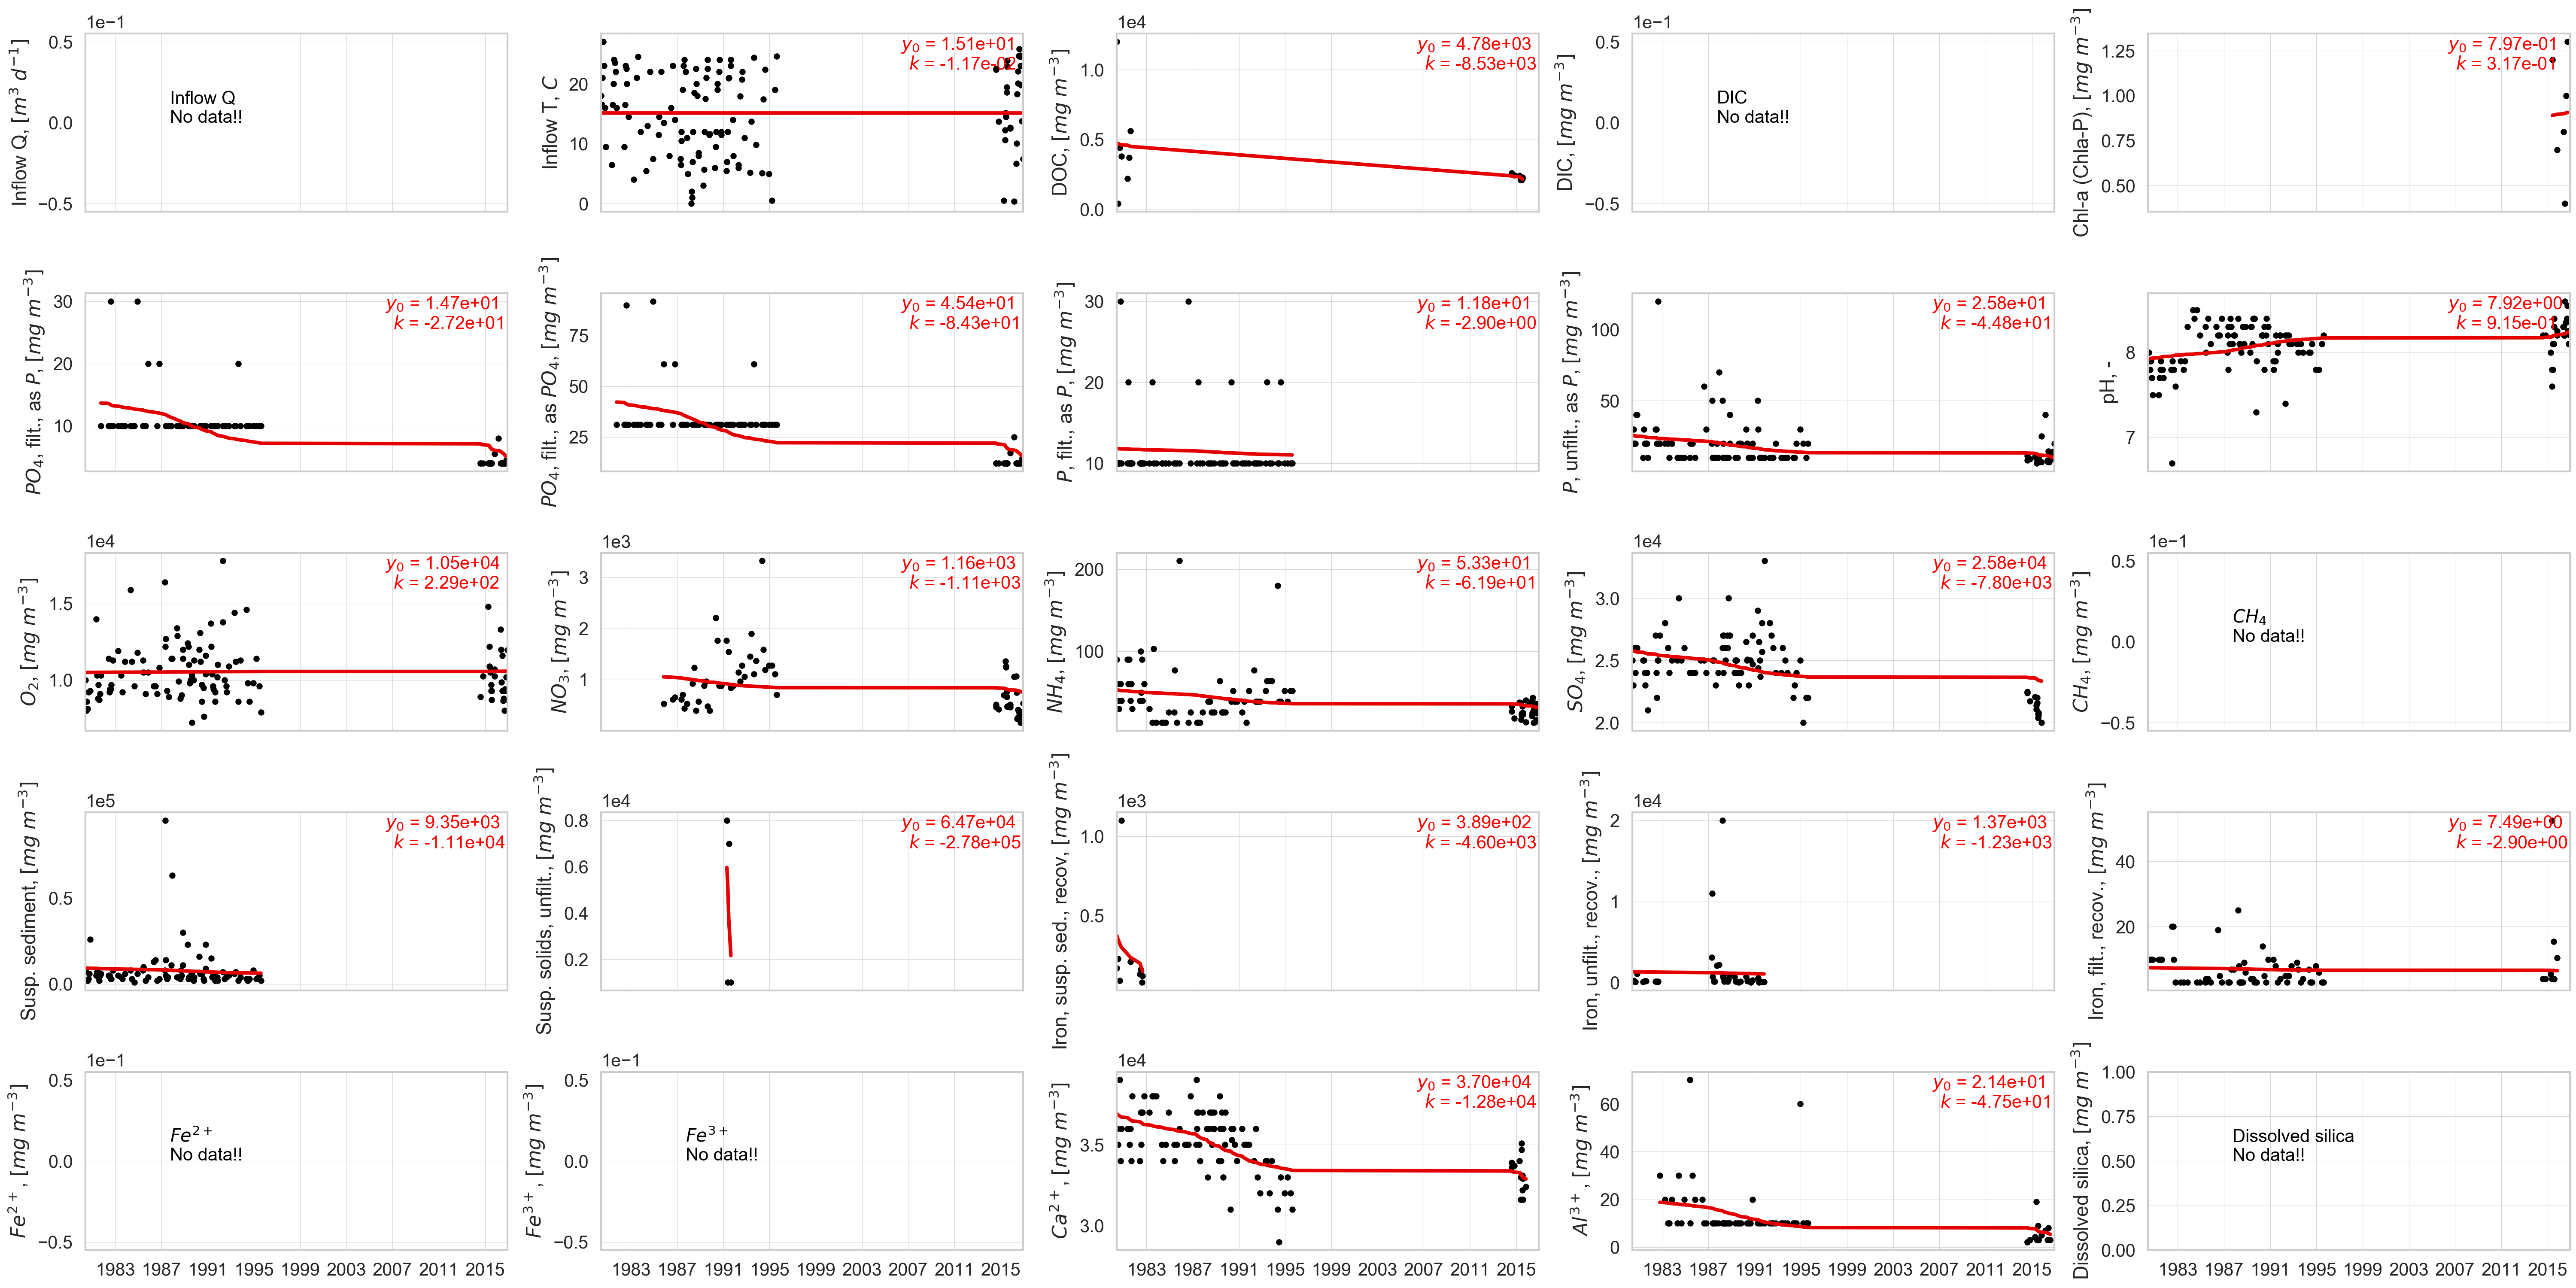
\includegraphics[width=\textwidth]{rivers/Western basin/niagarariver.png}
\end{figure}

\end{frame}

\begin{frame}
\frametitle{Eastern Basin: Buffalo creek}

\begin{figure}
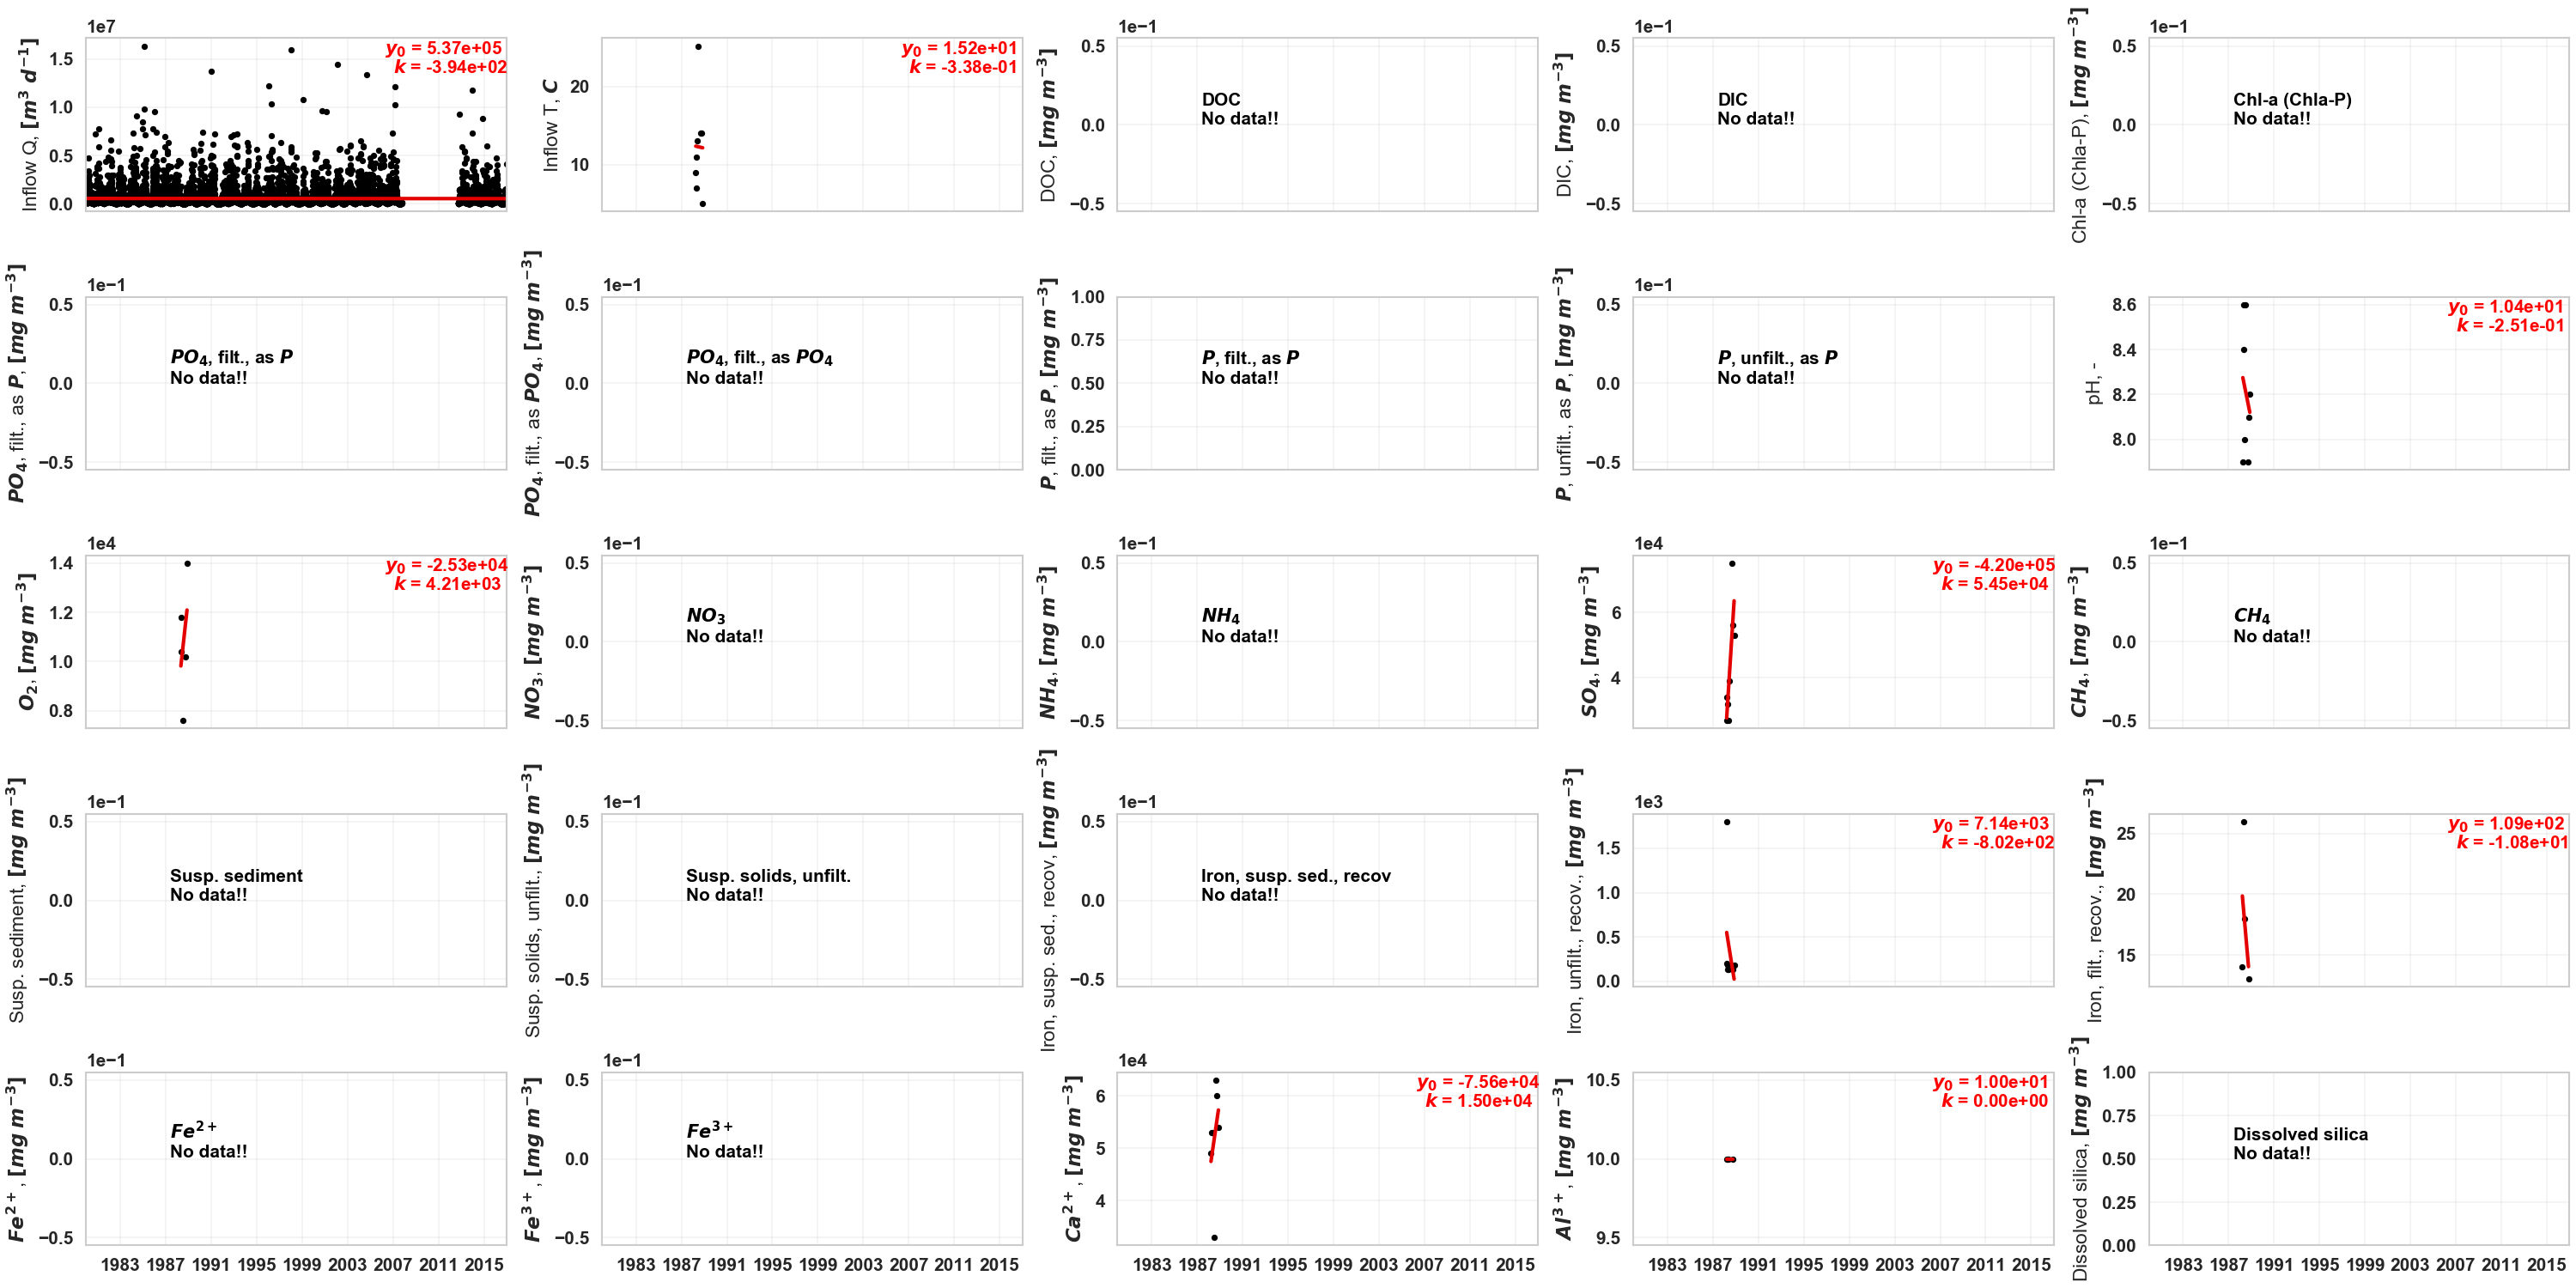
\includegraphics[width=\textwidth]{rivers/Eastern basin/Buffalocreek.png}
\end{figure}

\end{frame}

\begin{frame}
\frametitle{Eastern Basin: Cattaraugus creek}

\begin{figure}
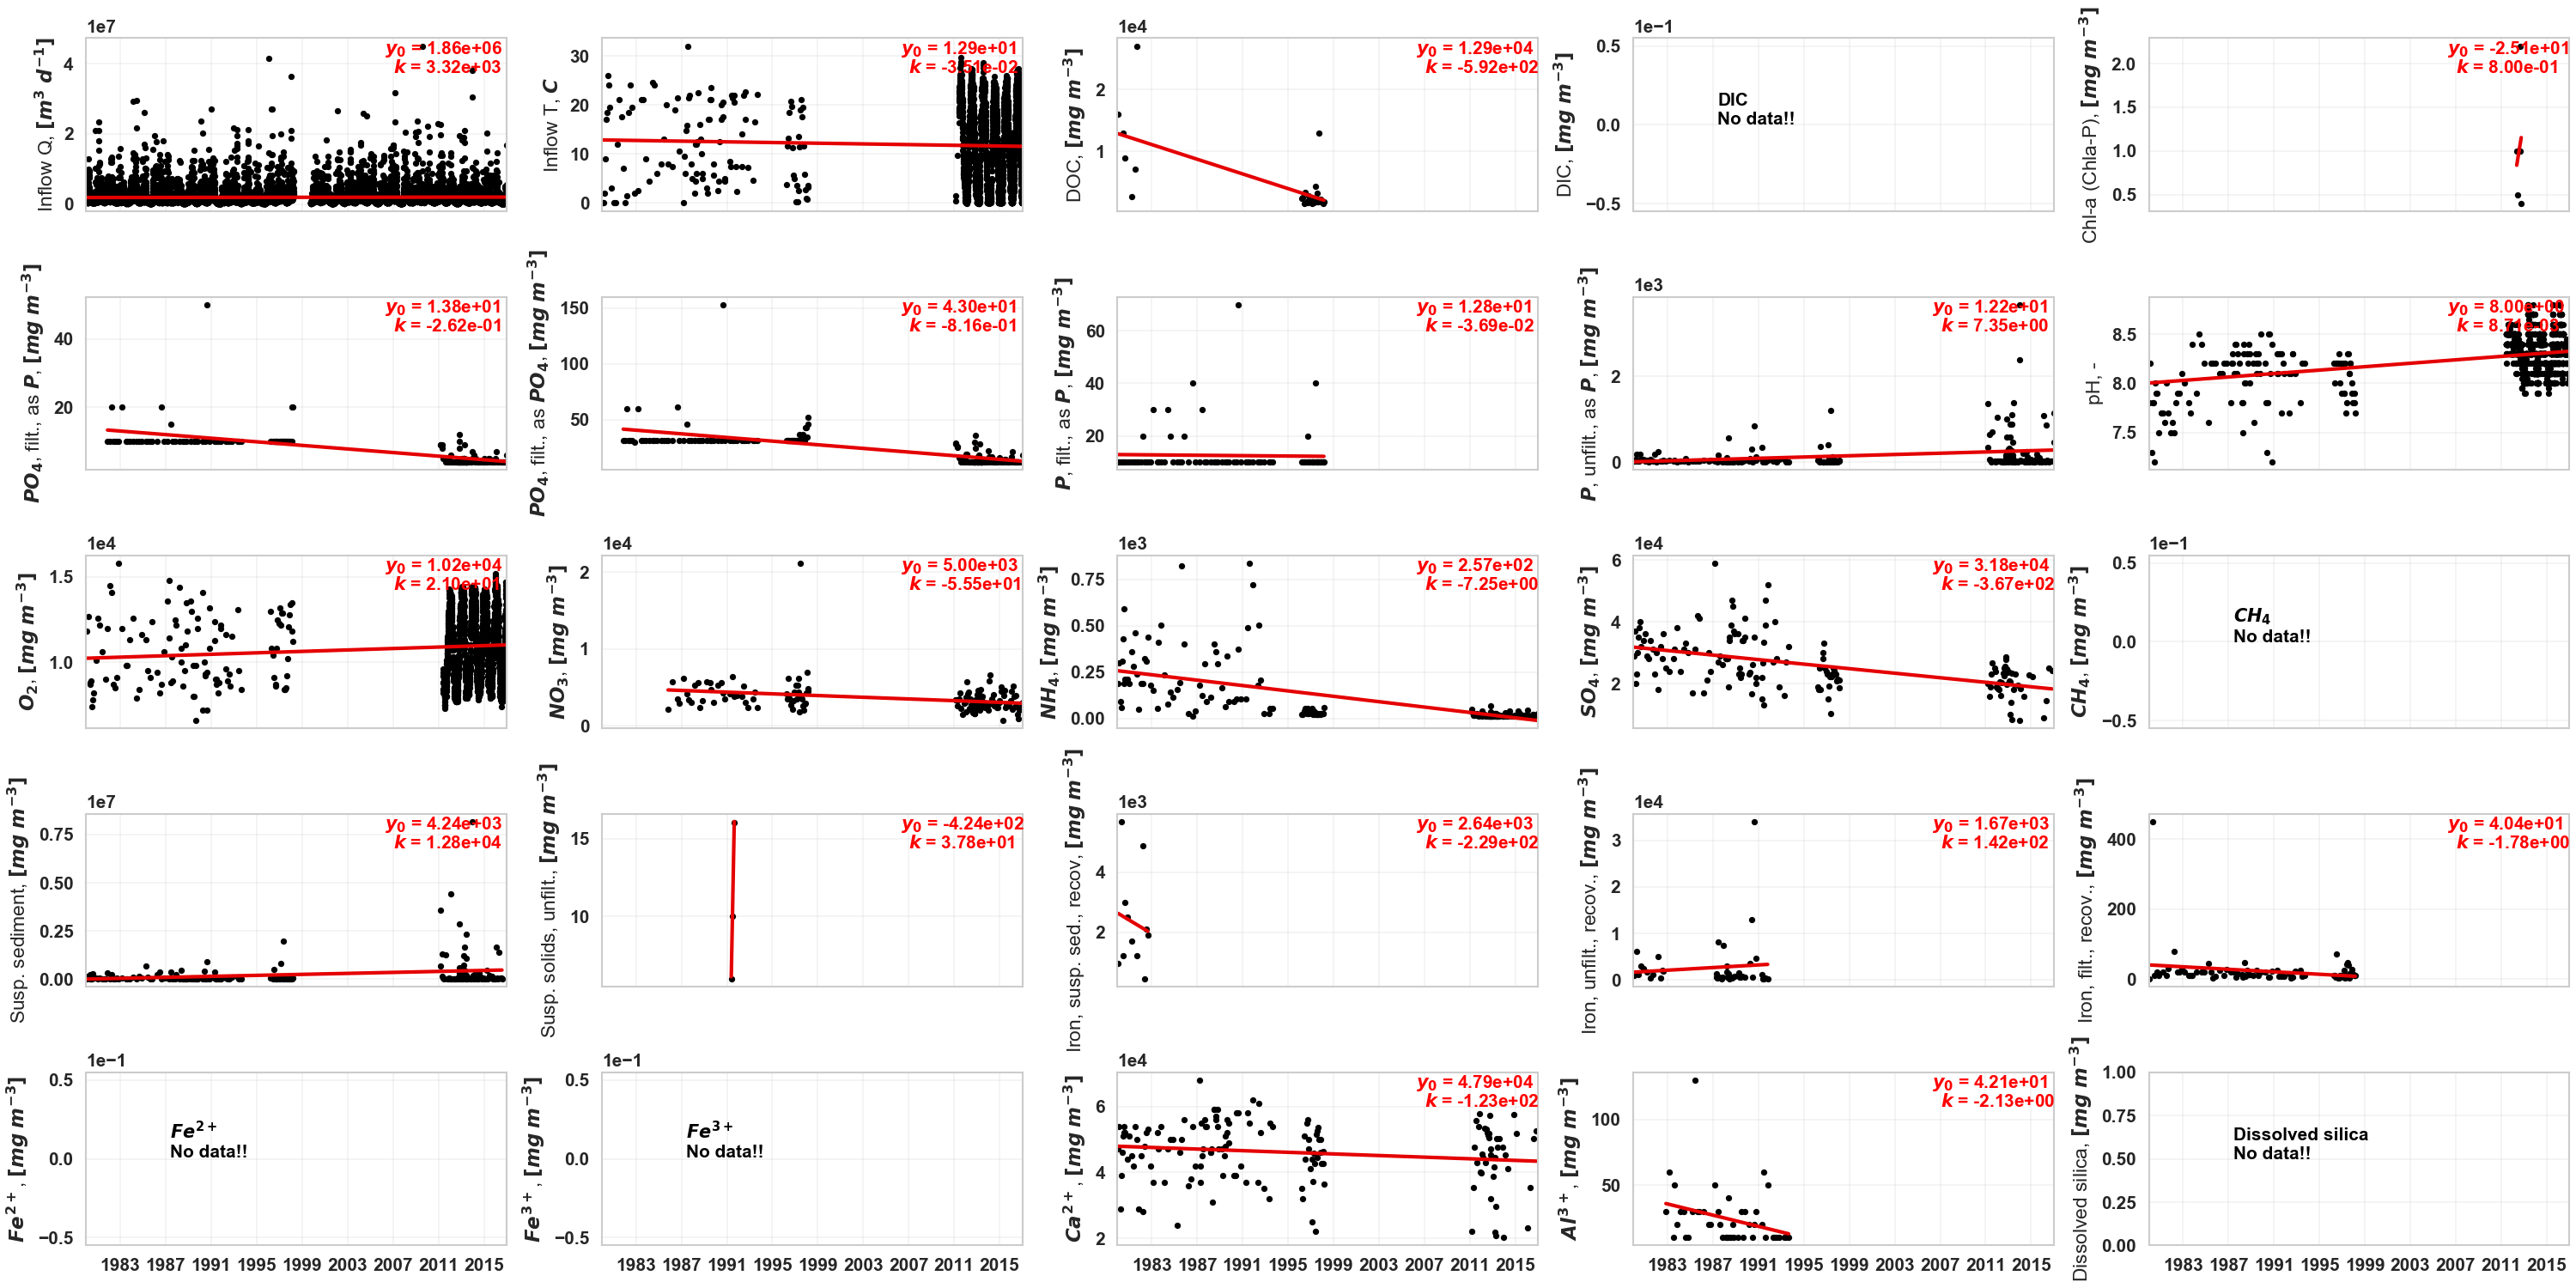
\includegraphics[width=\textwidth]{rivers/Eastern basin/cattarauguscreek.png}
\end{figure}

\end{frame}

\end{document}
